\documentclass[a4paper]{report}
\usepackage[utf8]{inputenc}
\usepackage{amssymb}
\usepackage{amsmath}
\usepackage{amsthm} 
\usepackage{url}
\usepackage{xspace}
\usepackage{graphicx}
\usepackage[vlined]{algorithm2e} % lib for pseudo code
\usepackage{float}  % lib for pseudo code
\usepackage[T1]{fontenc}
\usepackage{pgfplots}
\usepackage{caption}
\usepackage{subcaption}
\usepackage{array}
\usepackage{mdframed}
\usepackage{rotating}
\usepackage{multirow}
\usepackage{dirtytalk}
\usepackage{longtable}
\usepackage[titletoc]{appendix}
\usepackage{hyperref}

\usepackage{listings}
\usepackage{color}

%New colors defined below
\definecolor{codegreen}{rgb}{0,0.6,0}
\definecolor{codegray}{rgb}{0.5,0.5,0.5}
\definecolor{codepurple}{rgb}{0.58,0,0.82}
\definecolor{backcolour}{rgb}{0.95,0.95,0.92}
\definecolor{lightgray}{rgb}{.9,.9,.9}
\definecolor{darkgray}{rgb}{.4,.4,.4}
\definecolor{purple}{rgb}{0.65, 0.12, 0.82}

\lstdefinelanguage{JavaScript}{
  keywords={typeof, new, true, false, catch, function, return, null, catch, switch, var, if, in, while, do, else, case, break},
  keywordstyle=\color{blue}\bfseries,
  ndkeywords={class, export, boolean, throw, implements, import, this},
  ndkeywordstyle=\color{darkgray}\bfseries,
  identifierstyle=\color{black},
  sensitive=false,
  comment=[l]{//},
  morecomment=[s]{/*}{*/},
  commentstyle=\color{purple}\ttfamily,
  stringstyle=\color{red}\ttfamily,
  morestring=[b]',
  morestring=[b]"
}

%Code listing style named "mystyle"
\lstdefinestyle{mystyle}{
  backgroundcolor=\color{backcolour},   commentstyle=\color{codegreen},
  keywordstyle=\color{magenta},
  numberstyle=\tiny\color{codegray},
  stringstyle=\color{codepurple},
  basicstyle=\footnotesize,
  breakatwhitespace=false,         
  breaklines=true,                 
  captionpos=b,                    
  keepspaces=true,                 
  numbers=left,                    
  numbersep=5pt,                  
  showspaces=false,                
  showstringspaces=false,
  showtabs=false,                  
  tabsize=2
}

%"mystyle" code listing set
\lstset{style=mystyle}


%Setup of the TableOfContent to incl. subsubsection
\setcounter{tocdepth}{3}
\setcounter{secnumdepth}{3}

\RestyleAlgo{boxruled}
\LinesNumbered


\newcolumntype{L}[1]{>{\raggedright\let\newline\\\arraybackslash\hspace{0pt}}m{#1}}

\graphicspath{ {Graphics/Images/} }

\usepackage{newunicodechar}
\newunicodechar{∙}{\cdotp}

\newcommand{\parahead}[1]{{\vspace*{6pt}\noindent\textbf{#1}\xspace\xspace\xspace\xspace}}

\newcommand{\heading}[1]{{\vspace{6pt}\noindent\sc{#1}}}

% Command for making <--> arrow with text above
\makeatletter
\newcommand\xleftrightarrow[2][]{%
  \ext@arrow 9999{\longleftrightarrowfill@}{#1}{#2}}
\newcommand\longleftrightarrowfill@{%
  \arrowfill@\leftarrow\relbar\rightarrow}
\makeatother

\newcommand{\dotp}[2]{\ensuremath{\left\langle {#1},{#2}\right\rangle}\xspace}
\newcommand{\Z}{\ensuremath{\mathbb{Z}}\xspace}
\newcommand{\Zq}{\ensuremath{\Z_q}\xspace}
\newcommand{\ZqStar}{\ensuremath{\Z_q^*}\xspace}
\newcommand{\Zp}{\ensuremath{\mathbb{Z}_p}\xspace}

\def\polyfactor{n\, \log_2^2 n}
\newcommand{\bigO}[1]{\ensuremath{\mathcal{O}\left(#1\right)}\xspace}
\renewcommand{\O}[1]{\ensuremath{{\mathcal{O}\left(#1\right)}}\xspace}


\theoremstyle{plain}
\newtheorem{thm}{Theorem}[subsection]
\newtheorem{lemma}{Lemma}[subsection]

\mdfdefinestyle{defstyle}{frametitlerule=true, frametitlerulewidth=0px}
\mdtheorem[style=defstyle]{defi}{Definition}[subsection]

\mdtheorem[style=defstyle]{infobox}{}[subsection]

\begin{document}

%***************************************************************
%               Title Page
%***************************************************************
\begin{titlepage}

\newcommand{\HRule}{\rule{\linewidth}{0.5mm}} % Defines a new command for the horizontal lines, change thickness here

\center % Center everything on the page
 
%----------------------------------------------------------------------------------------
%	HEADING SECTIONS
%----------------------------------------------------------------------------------------

\textsc{\LARGE Aalborg university}\\[0.5cm] % Name of your university/college
\textsc{\large Department of Mathematical Sciences}\\[1.5cm] %Minor Heading 
\textsc{\Large Master of IT, Software Development}\\[0.5cm] % Major Heading
\textsc{\large Master thesis}\\[0.5cm] %Minor Heading 

%----------------------------------------------------------------------------------------
%	TITLE SECTION
%----------------------------------------------------------------------------------------

\HRule \\[0.4cm]
{ \huge \bfseries Electronic voting application based on public verifiable secret sharing}\\[0.4cm] % Title
\HRule \\[1.5cm]
 
%----------------------------------------------------------------------------------------
%	AUTHOR SECTION
%----------------------------------------------------------------------------------------

\begin{minipage}{0.4\textwidth}
\begin{flushleft} \large
\emph{Author:}\\
Sune Chung \textsc{Jepsen} % Your name
Kasper Jensen \textsc{Lemming} % Your name
\end{flushleft}
\end{minipage}
~
\begin{minipage}{0.4\textwidth}
\begin{flushright} \large
\emph{Supervisor:} \\
Ignacio \textsc{Cascudo} % Supervisor's Name
\end{flushright}
\end{minipage}\\[2cm]

% If you don't want a supervisor, uncomment the two lines below and remove the section above
%\Large \emph{Author:}\\
%John \textsc{Smith}\\[3cm] % Your name

%----------------------------------------------------------------------------------------
%	DATE SECTION
%----------------------------------------------------------------------------------------

{\large June 2017}\\[2cm] % Date, change the \today to a set date if you want to be precise

%----------------------------------------------------------------------------------------
%	LOGO SECTION
%----------------------------------------------------------------------------------------


\includegraphics{AAU_LOGO.png}\\[1cm] % Include a department/university logo - this will require the graphicx package
 
%----------------------------------------------------------------------------------------

\vfill % Fill the rest of the page with whitespace

\end{titlepage}
\chapter*{Acknowledgements}

It has been a learning period for the past six months, where we have studied the public verifiable secret sharing protocol. It has been a steep learning curve, but as we have worked with the topics on  a theoretical and practical level, we have gained an understanding of the protocol and its application.\\

\noindent
We would like to express our gratitude to our supervisor Ignacio Cascudo for his guidance and expert knowledge on this area throughout our work with this Master thesis. 

\chapter*{Summary}
In this Master thesis we will study the public verifiable secret sharing protocol and how it can be used in an electronic voting application based on the work from \cite{Schoenmakers1999}. Based on this knowledge we will design an implement a web based electronic voting application.\\

\noindent
Our work with this protocol leads to the following main topics which should cover our objective about Shamirs secret sharing, multiparty computation, public verifiable secret sharing protocol and our implementation of an electronic voting application.

\begin{enumerate}
    \item Voting
    \item Mathematical understanding
    \item Multiparty computation
    \item Electronic voting protocol
    \item Designing the application
    \item The application
    \item Reflection
\end{enumerate}

\noindent
We start to describe the concept of electronic voting and the challenges with the different types of electronic voting applications. We will use other studies and their demands for concrete security requirements, which we can include in our consideration for our electronic voting application.  \\

\noindent
To understand the public verifiable secret sharing protocol one need some basic mathematical understanding and some knowledge about cryptographic tools. Modular arithmetic and group theory will be key elements in understanding how the protocol works. Regarding to the cryptographic tools we will present the discrete logarithm problem which is the security primitive for this protocol.\\

\noindent
The public verifiable secret sharing protocol is an extension of multiparty computation protocol. Since the multiparty computation protocol uses secret sharing we need a basic understanding on these two subjects. Multiparty computation is basically about allowing parties to compute some function on some private inputs, in such a way that they learn the result but not the inputs from the other parties. Regarding secret sharing is about hiding information in a random polynomial. By using this polynomial, parties can create shares based on evaluations in the polynomial. If enough parties then collect their shares together they will be able to recover the secret.  We will present a simple secret sharing example which illustrate how a secret can be distributed and reconstructed. In addition to these properties the public verifiable secret sharing protocol gives us the ability to publicly verify the validity of the shares among the parties involved in this protocol. This means that the protocol is secure against malicious parties which try to send votes which they are not supposed to do. \\

\noindent
The electronic voting protocol part is splitted into two part a basic and a more in depth description of the protocol. The first part is intended to a developer who can implement a basic part of the protocol. The second part is a more in depth part on the verifying part of the protocol and the mathematical justification of why it works. \\   


\noindent
Designing the application is about our architectural strategies for our application based on the knowledge from literature from \cite{Bass} and \cite{Baerbak10}. We took the security requirements from the previous as the demands for our application. To extract the architectural demands, such as interoperability, modifiability and testing, for our application we will use Quality attribute scenarios which is a way of defining a clear architectural measurable demands. In addition for these demands we support this with diagrams which show the influence on the architecture of the application. The process of deriving these demands is done through an Quality attribute workshop. Since we are in  limited  time we only use the structure of the Quality attribute workshop for deriving the Quality attributes scenarios. Furthermore the structure of the workshop helped us prioritize among a long list of demands, which gave us the most important scenarios which we had to implement.\\


\noindent
The application is about giving an overview how our application is implemented with focus on the architectural elements. This part also contain our perspective of how well our application obeyed the security requirements. \\


\noindent
The reflection summarizes the most important reflections on our results from the theoretical and the practical parts of this thesis. 



  


 

\clearpage

\tableofcontents
\lstlistoflistings


\part{Introduction}
\clearpage
%***************************************************************
%               Part 1: Introduction
%***************************************************************
\chapter{Introduction}
    \section{Introduction}
\parahead{A MPC protocol}  allows several parties to compute some function on some private inputs, in such a way that they learn the result but not the inputs from the other players.  The challenge with MPC protocol is that it assumes that everyone is honest and sends correct data. \\


\parahead{In the Public verifiable secret sharing (PVSS protocol)} there is mechanisms to verify the correctness of the transmitted data.\\\\

\parahead{Secret sharing protocol} allows several parties to compute some function on some private inputs, in such a way that they learn the result but not the inputs from the other parties. When more than two parties want to share something secret, then they need some tools “Protocols” to make it possible. In this section we will look at secret sharing. We will look at sharing and reconstructing the secret from the shares - and how this can technically be possible. 

\parahead{Practical implementation} with focus on architecture. Skalerbarhed. Sikkerhed. Test. Performence. \\



\noindent
Man skal ikke være i tvivl om hvad vi vil arbejde med efter vores introduktionen, motivation og hypotese


    
    \section{Motivation} There are theoretical papers about how participants can communicate secure. For different reasons there are fewer papers which propose how to implement their theoretical results. It could be interesting to combine the knowledge we gained from our lectures in it-security and software architecture, to describe, design and implement a MPC protocol. In collaboration with our mentor we decided to study and implement the electronic voting solution based on the PVSS protocol describe in \cite{Schoenmakers1999}. In this solution we will have focus on designing a secure and scalable distributed architecture. Using known software design principle from \cite{Bass} and \cite{Baerbak10}, we discuss and reflect on different solutions.
    
    \section{Objectives}
This master thesis consist of two main parts. The first a theoretical background where we study the electronic voting protocol described in \cite{Schoenmakers1999}. In order to understand the protocol, some study in the basic field of cryptography is required. In the second part of the project, we will try to design and implement a web based electronic voting application based on the protocol. Basically this master thesis have the following objectives. 

\begin{enumerate}
    \item   Describe the theory behind Shamirs secret sharing and multiparty computation as well as the cryptographical concepts needed to understand it. The aim is to describe the theories clearly and with examples such that one really understand how it works. 
            
    \item   Describe the electronic voting protocol \cite{Schoenmakers1999} and the mathematically justification behind it, again aiming to describe the protocol clearly and with examples to really understands how it works.
    
    \item   Design and implement a secure and scalable web based electronic voting application based on the protocol. Known software design principles will be used to acquire high and reliable software quality.
    The aim is to make the application web based, such that it is easily accessible to a broad audience.
\end{enumerate}



    
    \section{Limitations}

The following limitations have be identified.

\begin{enumerate}
    \item The field of multiparty computation if broad and there exist numerous of scientific papers describing different protocol. This thesis will only focus on the main concepts in order to understand
    the eletronic voting protocol. 
    
    \item The application designed and developed in this thesis are to be 
\end{enumerate}
    
    \section{Overview}
Here we present the content of the rapport. One section will contain the mathematical description of the protocol. The second section will be about the pratical part of the voting application, where we will descripe an our implementation.

\part{Theoretical}
 \clearpage
%***************************************************************
%               Part 2: Voting
%***************************************************************  
\chapter{Voting} \label{chap:voting}    
    In this chapter we will briefly describe electronic voting in general. In order to develop an electronic voting application, its important to understand the challenges and secure parameters for an electronic voting. This knowledge will help us define system requirements for the design of the electronic voting systems. And it will ultimately serve as parameters which we can hold our implementation accountable. 


\section{Introduction}
In many aspects of our life's we encounter the act of voting, from simple things as voting whats for dinner, to the more complex things as a government election. The later involving a large number of people from different geographical locations. These election is normally handled by dividing the people into sections based on location, each section handling it's own sub-election and submitting the result to a overall tally. Though many countries still mostly rely on the old fashioned paper based ballots, we have in the recent years seen an increase in electronic voting. Electronic voting refers to the act of voting though an electronic devices and depending on the voting equipment and location, it can be divide into five categories \cite{Cet09}. 

\section{Classification}

\begin{description}
\item[DRE voting] Direct Recording Electronic is a specialized standalone electronic voting machine, which have the attributes of being physically hardened and have software specifically for voting installed. Votes casted on a DRE is do within a voting booth located on a polling site, and the votes is then recorded into a electronic ballot box.

\item[Poll-site voting] The voting is located on a polling site, votes are cast on public computers located on the site, in favour for voting booths. The computers on site are connected to a counting authority server though a closed and controlled network. Authentication can be done prior to the voting period or at the polling site

\item[Poll-site kiosk voting] Votes are casted inside a voting booth located at a polling site, using a terminal. The terminal is connected to a counting authority server though a closed and controlled network. Authentication is done at the polling site before allowed access to the voting booth. 

\item[Poll-site Internet voting] Votes are casted on public computers located on a polling site. The public computers on site is online and connected to a counting authority server over uncontrolled network. Authentication can be done prior to the voting period or at the polling site

\item[Remote Internet voting] Simply requires internet access and can be done from a home computer. Authentication is done prior to the voting an typical involves password or some type of authentication token. 

\end{description}


\section{The Voting Process}
Similar to the classification, there exist several of different systems and protocols for electronic voting. But they typically all follows the same process and includes the same actors as illustrated and describe below \cite{Cet09}. 

\begin{figure}[H]
\centering
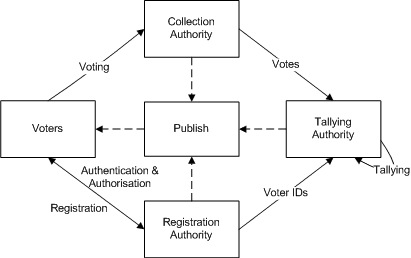
\includegraphics[scale=0.7]{Voting_Process.png}

\caption{Voting process}
\label{fig:Voting_Process}
\end{figure}

\begin{description}
    \item[Voter] Voter refers to a person who is eligible and who has registered for the privileges of voting in a given election. 
        
    \item[Registration authority] Registration authority refers to the authority that is responsible for registering eligible voters, and ensuring that only these voters are allowed to vote. Furthermore they ensures that voters only vote ones. 
        
    \item[Collection authority] The collection authority refers to the authority that is responsible for properly collecting all the votes. This authority can be represent as a simple electronic ballot box.

    \item[Tallying authority] Tallying authority are responsible for counting the votes of the election and publishing the result. 
\end{description}


\noindent
The voting process as illustrated on figure \ref{fig:Voting_Process} holds true for any voting system, and includes four stages. 

\begin{description}
    \item[Registration] Prior to an election, people who are eligible for voting, signs up to vote in the election. These voters are then registered, thus hereby ensuring no double voting acquires.
        
    \item[Authentication and Authorisation] Registered voters are authenticated, if they are found eligible and have not voted yet. Ones authenticated, the voter is giving access to cast his vote in the election.  
        
    \item[Voting] The voters cast there votes. 

    \item[Tallying] In this final stage the votes are counted, and of course only valid votes are being included. Ones the counting process is finished the final count is published. 
\end{description}


\section{Challenges}
Though the process of electronic voting have many similarities with paper based voting systems, there is still concern of the security. In paper based voting systems, the security is easily noticeable as this is represented by officials observing every stages of the process. the process typically goes along the lines of: When arriving to the polling site a voter typically already have proofs that he is eligible and is simply registered and handed the paper ballots. The paper ballot is fulfilled in a voting booth where only the voter himself is present. When the ballot is fulfilled, it is folded or put in an envelope, in order to hide the vote, and then put in a ballot box located on the polling site. Note that ballot is anonymous and typical only requires a simple mark. Ones all the votes have been cast or a deadline is reached then the votes is counted. Throughout this entire process there are neutral officials physical present typically along with represents from each party in the election and passive observers.   \\

\noindent
In electronic voting systems the security is not this visible and if the system falls into the classification of \textit{Poll-site Internet voting} or \textit{Remote Internet voting} then uncontrolled network is used and the group of potential adversary is significantly increased.
To ensure security and public trust an electronic vote system should aim to fulfill the goals 
listed below \cite{Damgaard2003}

\begin{description}
    \item[Privacy] Throughout the process no information should be leaked, only the final counting
    should be made public. At no time should a vote could be linked to the voter. 
    
    \item[Robustness] The system should be tolerant against cheating. Only valid and correctly fulfilled ballots should be counted. Nobody should be able to manipulating the final count.

    \item[Universal verifiability] The final count should be public verifiable. Anyone should be able to convince himself of the fairness of the election. This should be done without gain any other information.
        
\end{description}

\section{Security Requirements} \label{sec:security_requirements}
The previous three goals are fairly board and can with benefit be specified into concrete security requirements as done in \cite{Cet08}

\begin{itemize}
    \item \textit{Voter Privacy}
        No one should be able to link a vote back to the specific voter, and only the voter should
        know his vote. These requirements shall hold during and after the election.  
    
    \item \textit{Eligibility}    
        Only Eligible and registered voters can vote. 
    
    \item \textit{Uniqueness}
        Only one vote per registered voter should be counted.
    
    \item \textit{Fairness}
        None should be able to gain any knowledge of the outcome of the election, before the ending. This is to prevent voters of voting accordingly to any leaked information. 
    
    \item \textit{Uncoercibility}
        Nobody should be able to extract the value of a vote. This is to prevent anybody from compelling a voter by force, intimidation, or authority to cast a vote in a specific way. 
    
    \item \textit{Receipt-freeness} 
        The voting system should not produce a receipt that reveals any information about the casted vote. This is to prevent a vote from trading his vote. 
    
    \item \textit{Accuracy} 
        The final tally should be correctly computed from valid casted votes. It should not be
        possible to manipulate the final tally without being detected. 
    
    \item \textit{Universal Verifiability}
        It should be possible for any participants and observers to validate individual votes as well as the final tally of the election. 
    
    \item \textit{Individual Verifiability}    
        Every registered voter should be able to verify that his vote is counted correctly. 
    
\end{itemize}


\section{Approaches}
To construct a electronic voting system that fulfills these security requirements, we look that three cryptographical techniques as follows 

\begin{description}
    \item[Blind signatures]

    \item[Mix-nets]        
        
    \item[Homomorphic encryption]
\end{description}

This that are to be detailed in this chapter: 

\begin{description}
    \item[Voter]
    \item[Tallier]
    \item[Observer]
    \item[Bulletin board]
\end{description}


\clearpage
%***************************************************************
%               Part 3: Mathematical understanding
%***************************************************************
\chapter{Mathematical understanding}
    In this chapter we describe the mathematical concepts and theories behind the electronic voting protocol. As we do not except the reader to have a fully comprehensive mathematical background, we will be describing the required concepts and theories here.
    
    \section{Method}
To ensure structure the sections will be contructed based one or more of the following 3 methods.
\begin{enumerate}
    \item \textbf{General structure}  \\
    Informal description\\
    Definition\\
    Example\\
    Proof    
    \item \textbf{Zero-knowledge proof}
    \item \textbf{Pseudo code} 
\end{enumerate}

\parahead{General structure} The general rule will be that every section will start informal description of the subject. Here we will give a informal description of why this it is relevant to our rapport. After that a more formal description will come. Their will be parts where the formality will require a more in depth explanation. To avoid disruption we then put this formality last in the section.    


\parahead{Zero knowledge proof} In cryptography, a zero-knowledge proof is a protocol by which one party (the prover) can prove to another party (the verifier) that a given statement is true, without revealing any information apart from the fact that the statement is indeed true.


\parahead{Pseudo code} We will use pseudocode as an informal technique to outline the structure of our algorithms. This technique aims to describe a solution so that it is easy to read for humans.




    
    \section{Modular arithmetic}
Modular arithmetic, is a simple way of performing arithmetic in a finite set of integers.

%**************************************Definition Modulo Operation Start
\begin{defi}[\textbf{Modulo Operation}]
Let \begin{math} a, r,m \in  \mathbb{Z}\end{math} (where \begin{math} \mathbb{Z}\end{math} is a set of all integers) and \begin{math} m > 0\end{math} and we write  
\begin{center} \begin{math} a = r \ mod \ m\end{math} \end{center}
if \begin{math}m \end{math} divides \begin{math} a - r \end{math}.\\
\begin{math}m \end{math} is called the modulus and \begin{math}r \end{math} is called the remainder.
\end{defi}
%**************************************Definition Modulo Operation End

\parahead{Computing the remainder} By example we can compute the remainder according to the definition. Given: \begin{math} a, m \in \mathbb{Z} \end{math} we compute the remainder by the following fomular:  \begin{math} a = qm +r \end{math}. The remainder is computed by how many times the quotient can be multiplied with the modulo. This example shows that the remainder is not unique. \\\\
\begin{math}42 = 4 * 9 +6 \implies r = 6 \end{math}, by definition \begin{math} (42-6) = 36 \end{math}, \begin{math} 9| 36 \end{math}\\
\begin{math}42 = 3 * 9 +15 \implies r = 15 \end{math}, by definition \begin{math} (42-15) = 27 \end{math}, \begin{math} 9| 27 \end{math}\\
\begin{math}42 = 5 * 9 +(-3) \implies r = -3 \end{math}, by definition \begin{math} (42-(-3)) = 45 \end{math}, \begin{math} 9| 45 \end{math}\\

\parahead{Equivalence classes} Above can also be written with the modulo operator. Here we show that all have different remainder but are in the same equivalence class modulo \textit{9}. This means that all members of a given equivalence class behave equivalently. Note also that one can compute with negative integers.

\begin{align*}
42 &= 6 \ mod \ 9 \\
42 &= 15 \ mod \ 9 \\
42 &= -3 \ mod \ 9 
\end{align*}

\parahead{Computing the inverse}
As we will see later, computing the inverse becomes an important part in this protocol for how to divide modulo an integer arithmetically. For this we have the Extended Euclidean algorithm which allows us to compute modular some integers. This computation results in computing the inverse.


\parahead{Extended Euclidean algorithm} To compute the inverse means that we want to compute the following \begin{math}a\ \cdot \ a^{-1} \ mod \ q = 1 \end{math} where $a, \ a^{-1}, \ q$ are integers and $a^{-1}$ is the inverse of $a$. The condition for the existence of the inverse is that the $gcd(q,\ a)= 1$. So if $gcd(q,\ a)= 1$ the Extended Euclidean Algorithm computes the inverse of $a$.\\


\noindent
\parahead{Explanation of the Extended Euclidean algorithm (EEA)} Since we will use an implementation in our electronic voting application we will explain the EEA by example. The first two lines (6-7) in the algorithm is the standard Euclidean Algorithm. It turns out that if we give the Extended Euclidean Algorithm $gcd(n,a)$, where $n$ is the modulo integer and $a$ is an integer, then the $t$ parameter will be the inverse of $a$. 

%**************************************Pseudocode Euclidean algorithm start
\begin{center}
\begin{algorithm}[H]
\caption{Extended Euclidean Algorithm (EEA)\label{alg}}

\SetKwRepeat{Do}{do}{while}

\KwIn{positive integers $r_0 $ and $r_1 $ with $r_0 $ > $r_1 $}
\KwOut{gcd($r_0 $, $r_1 $), as well as s and t such that gcd($r_0$, $r_1$) = $s * r_0+t * r_1 $.}

\textbf{Initialization:} \\
$
\begin{array}{ll}
    s_0 = 1   & t_0 = 0 \\
    s_1 = 0   & t_1 = 1 \\
      i = 1     &           \\
\end{array}                 
$

\Begin{
    \Do{$r_i \neq 0 $}{
    $i = i+1 $\\
    $r_i = r_{i-2} \ mod \ r_{i-1} $\\
    \begin{math} \mathbf{ q_{i-1} = ( r_{i-2}-r_{i} ) / r_{i-1} }  \end{math}\\
    $s_i = s_{i-2}-q_{i-1} * s_{i-1} $\\
    $t_i = t_{i-2}-q_{i-1} * t_{i-1} $
    }

\Return{ \\
    gcd($r_0 $, $r_1 $) = $r_{i-1} $\\
    s = $s_{i-1} $\\
    t = $t_{i-1} $
    }
}
\end{algorithm}
\end{center}


%**************************************Pseudocode Euclidean algorithm end
\noindent
The regular Euclidean algorithm works that given to integers $r_0 = 911$ and $r_1 = 301$. The gcd is computed by reducing the problem of finding the gcd of two given numbers to that of the gcd of two smaller numbers 


\begin{center}
\begin{tabular}{|ll|lll| } 
\hline
$911$ & $= 3 \cdot 301 +8$& $gcd(911,301)$ & $= gcd(301,8)$ & \\ 
\hline
$301$ & $= 37 \cdot 8+5$ & $gcd(301,8)$ & $= gcd(8,5)$ &\\ 
\hline
$8$ & $= 1 \cdot 5+3$ & $gcd(8,5)$ & $= gcd(5,3)$ & \\ 
\hline
$5$ & $= 1 \cdot 3+2$ & $gcd(5,3)$ & $= gcd(3,2)$ & \\ 
\hline
$3$ & $= 1 \cdot 2+1$ & $gcd(3,2)$ & $= gcd(2,1)$ & \\ 
\hline
$2$ & $= 1 \cdot 1+1$ & $gcd(2,1)$ & $= gcd(1,1)$ & \\ 
\hline
$1$ & $= 1 \cdot 1+0$ & $gcd(1,1)$ & $= gcd(1,0)$ & $= 1$ \\ 
\hline
\end{tabular}
\end{center}


\noindent
\parahead{Example Extended Euclidean algorithm} The main point is that the last iteration we computed the parameter $t$, from two previous iterations. This $t$ parameter is the inverse of $r_1$. On the left-hand side, we compute the standard Euclidean algorithm, i.e., we compute new remainders $r_2$, $r_3$, ... Also, we have to compute the integer quotient $q_{i-1}$ in every iteration. On the right-hand side we compute the coefficients $s_i$ and $t_i$ such that $r_i = s_i r_0 + t_i r_1$. 
\begin{center}
\begin{tabular}{|l|l|p{5cm}| } 
\hline
$i$ & $r_{i-2} = q_{i-1} \cdot r_{i-1}+r_i$ & $r_i = [s_i]r_0 +[t_i]r_1$ \\ 
\hline
$2$ & $911 = 3 \cdot 301 +8$& $r_2=8= [1] 911 + [-3]301$ \\ 
\hline
$3$ & $301 = 37 \cdot 8+5$ & $r_3= 5= 301-37 \cdot 8$ \newline $ r_3 = 301 -37(911-3 \cdot 301)$ \newline $r_3 = -[37]911 + [112]301$\\
\hline
$4$ & $8 = 1 \cdot 5+3$ & $r_4= 3 = 8-5$ \newline $r_4 = 1 \cdot 911 + (-3) \cdot 301 - (-37 \cdot 973 + 112 \cdot 301)$ \newline $r_4 = [38]911 - [115]301$  \\
\hline
$5$ & $5 = 1 \cdot 3+2$ & $r_5= 2= 5-3$ \newline $r_5=-37 \cdot 911 + 112 \cdot 301 - (38 \cdot 911 - 115 \cdot 301)$  \newline  $r_5 = -[75]911 + [227]301$ \\
\hline
$6$ & $3 = 1 \cdot 2+1$ & $r_6= 1 = 3-2$ \newline $r_6=38 \cdot 911 - 115 \cdot 301 -(-75 \cdot 911 +  227 \cdot 301)$ \newline $r_4=[113]911-[342] 301$  \\ 
\hline
$7$ & $2 = 1 \cdot 1+1$ & $r_7= 1 = 2-1$ \newline $r_7=-75 \cdot 911 + 227 \cdot 301 -(113 \cdot 911- 342 \cdot 301)$ \newline $r_7=-[188]911+[569] 301$  \\ 
\hline
\end{tabular}
\end{center}


\noindent
To understand how the EEA works we observe that the righthand side is always constructed with the help of the previous linear combinations. We will now derive recursive formulae for computing $s_i$ and $r_i$ in every iteration. Assume we are in iteration with index i. 

\begin{infobox}[The two previous iterations we computed the values]
$r_{i - 2} = [s_{i-2}]r_0 +[t_{i-2}]r_1$\\
$r_{i-1} = [s_{i-1}]r_0 +[t_{i-1}]r_1$
\end{infobox}

\noindent
In the current iteration i we first compute the quotient $q_{i-1}$ and the new remainder $r_i$ from $r_{i-1}$ and $r_{i-2}$:

\begin{infobox}[Current iteration $i$]
$r_{i-2} = q_{i-1} \cdot r_{i-1}+r_i$.\\
This equation can be rewritten as:\\
$r_i = r_{i-2}-q_{i-1} \cdot r_{i-1}$.
\end{infobox}


\noindent
The goal is to represent the new remainder $r_i$ as a linear combination of $r_0$ and $r_1$ as $r_i = [s_i]r_0 +[t_i]r_1$. The core step for achieving this is by substitute $r_{i-2}$ and $r_{i-1}$ by the following.

\noindent
\begin{infobox}[General formula is derived by substitute $r_{i-2}$ and $r_{i-1}$]
$r_i = (s_{i-2}r_0+t_{i-2}r_1)-q_{i-1}(s_{i-1}r_0+t_{i-1}r_1)$\\
If we rearrange the terms we obtain the desired result:\\
$r_i = [s_{i-2}-q_{i-1}s_{i-1}]r_0 +[t_{i-2}-q_{i-1}t_{i-1}]r_1$\\
$r_i = [s_i]r_0 +[t_i]r_1$
\end{infobox}


    
    
\section{Group theory}
A computer cant work with infinite set. If we look at the set of reel numbers we have infinite numbers like $\frac{1}{3} = 0.33333...3$, we can therefor not work with reel numbers. We therefor turn to integers which we know dont have these types infinite representation. However the set is also infinite. We therefor need find a subset of integers which can form a finite group. We need this subset of integers to uphold certain properties. We start by looking at the definition of a general group \cite{Paar}.  

%-----------------------------------------------Definition of group start
\begin{defi}[\textbf{Group}]
A \textnormal{group} is a set \begin{math}\mathbb{G}\end{math} along with a binary operation \begin{math}\circ \end{math} for which the following conditions hold:.
\begin{itemize}
\item \textnormal{\textbf{(Closure:)}}  \begin{math} For \ all \ g, \ h \in \mathbb{G},\ g \circ h \in \mathbb{G} \end{math}.
\item \textnormal{\textbf{(Existence of an identity:)}} \begin{math} There \ exists \ an \end{math} \textnormal{identity} \begin{math} e \in \mathbb{G} \end{math} such that for  all \begin{math} g \in \mathbb{G}, e \circ g = g =g \circ e \end{math}
\item \textnormal{\textbf{(Existence of Inverses:)}} For all \begin{math}g \in \mathbb{G}\end{math} there exists an element \begin{math}h \in \mathbb{G}\end{math} such that \begin{math}g \circ h = e =h \circ g \end{math} such that an h is called an \textnormal{inverse} of g.
\item \textnormal{\textbf{(Associativity:)}} For all \begin{math}g_1, g_2, g_3 \in \mathbb{G}, (g_1 \circ g_2) \circ g_3 = g_1 \circ( g_2 \circ g_3) \end{math}
\end{itemize}
When \begin{math}\mathbb{G}\end{math} has a finite number of elements, we say \begin{math}\mathbb{G}\end{math} is a finite group and let
\begin{math}| \mathbb{G}|\end{math} denote the order of the group; that is, the number of elements in \begin{math}\mathbb{G}\end{math}. \\
A group \begin{math}\mathbb{G}\end{math} with operation \begin{math}\circ\end{math} is abelian if the following holds:
\begin{itemize}
\item \textnormal{\textbf{(Commutativity:)}} For all \begin{math}g, h \in \mathbb{G}, g \circ h = h \circ g \end{math}
\end{itemize}
\end{defi}
%-----------------------------------------------Definition of group end

\noindent
As we described above we should find a subset of integers which satisfies the group definition. By using modulo we define a subset of integers, as $G= \Zq $ where $q$ is an modulo integer. By example we see the following \begin{math} \Z_4 = \{0,1,2,3\}\end{math}   


\parahead{Closure} Closure means when we do operations in the set we always end up with an element from the set. that we always do computation in the set. The modulo operation ensures that we always reduce computations into a closed set.


\parahead{Existence of Inverses} The inverse means that we want to compute a number such that \begin{math}a\ \cdot x \ mod \ q = 1 \end{math}.  For the integers we have to ensure that the greatest commend divisor is 1 to ensure the inverse property. By example we see the following \begin{math} \Z_4 = \{0,1,2,3\}\end{math}. Removing all the numbers that does have a gcd with $4$ larger then $1$ gives set of $\Z_4^* = \{1,3\}$ . Note the star in the notation. This refers to a set with none greatest common divisor larger then $1$. If we take a prime we know that the gcd holds for every number up to the prime. So  \begin{math} \Z_7 = \{0,1,2,3,4,5,6\}\end{math} becomes \begin{math} \Z_7^* = \{1,2,3,4,5,6\}\end{math}. To compute the inverse we will use Extended Euclidean algorithm.


\parahead{Existence of an identity} There should always be a neutral element. When the operation is mulitplication the neutral element is $1$ and when the operation is addition the neutral element is $0$.

\parahead{Associativity} By example one can show that associativity holds. If we take $ \Z_{10}^*$ with the following two expressions $ (3 \cdot 7 \ mod \ 10) \cdot 9 \ mod \ 10 $ and  $ 3 \cdot ( 7 \cdot 9 \ mod \ 10) \ mod \ 10) $. This can be reduced to $ (3 \cdot 7 \ mod \ 10) \cdot 9 \ mod \ 10 = 1 \cdot 9 \ mod \ 10 = 9 \ mod \ 10$. This can be reduced to $ 3 \cdot ( 7 \cdot 9 \ mod \ 10) \ mod \ 10) = 3 \cdot 3 \ mod \ 10 = 9 \ mod \ 10 $.



\parahead{Cyclic group} A cyclic group is if the group contains at least one element (generator) with the order of the cardinality (number of elements) of the group. This can also be formulated as the maximum cycle length which is $p-1$, which means when the generator begins to repeat the elements it is said to be cyclic.

\parahead{Generators} An example of a generator could be the following. Let \begin{math}q=5\end{math} and \begin{math} \Z_q^*\end{math} be a group with \begin{math} \Z_q^* = \{1,2,3,...,q-1\}\end{math}. It can be seen that \begin{math} g=2\end{math} is a generator because,  \begin{math}2^1=2,\ 2^2=4,\ 2^3=8 \ (mod\ 5)=3,\ 2^4=16 \ (mod \ 5)=1 \end{math}, generates every element in the group. Here we see that $2$ have the maximum order $ord(2)=4$ of the group which i $4$ and therefor this group is said to be cyclic.

%-----------------------------------------------Definition of group start
\begin{defi}[\textbf{Cyclic Group}]
A group $G$ which contains an element $ \alpha $ with maximum order $ord( \alpha ) = |G|$ is said to be cyclic. Elements with maximum order are called generator.
\end{defi}
%-----------------------------------------------Definition of group end



\parahead{Field} The protocol uses finite field because the protocol uses Shamir secret sharing. Particular we are using field in the exponents where we are summing and multiplying. In the base we multiplying.  But before we can explain a finite field we should know a field. A field is a  algebraic structure which forms an additive group and multiplicative group  respectively with group operation addition and multiplication. Remember that a field also contains subtraction and division operator. Subtraction can be formulated through addition of a negative number. Division can be formulated as a multiplication between number an inverse.  
%-----------------------------------------------Definition of finite start
\begin{defi}[\textbf{Field}]
A field F is a set of elements with the following properties:
\begin{itemize}
\item  All elements of $F$ form an additive group with the group operation $+$ and the neutral element $0$.
\item  All elements of $F$ except $0$ form a multiplicative group with the group operation $ \cdot $ and the neutral element $1$.
\item When the two group operations are mixed, the distributivity law holds, i.e., for all $a,b,c \in F: a(b+c) = (ab)+(ac)$.
\end{itemize}
\end{defi}
%-----------------------------------------------Definition of finite end
\parahead{Finite field} A finite field is when one does operation in the set the result stays in the set. When we do operation e.g. do multiplication and uses modulo we will stay in the set.
%-----------------------------------------------Definition of finite fields start
\begin{defi}[\textbf{Finite fields}]
A finite field is a field $F$ which contains a finite number of elements. The order of $F$ is the number of elements in $F$.
\end{defi}
%-----------------------------------------------Definition of finite fields end


    
    \section{Cryptographic tools}
The following section will be about the cryptographic assumptions which are used in the PVSS protocol. We will also describe some techniques which will be used in practical part of coding the protocol.


%------------------------------------------------------------------------------------
\subsection{Zero knowledge proof} % Zero knowledge proof
%------------------------------------------------------------------------------------
In cryptography, a zero-knowledge proof is a protocol by which one party (the prover) can prove to another party (the verifier) that a given statement is true, without revealing any information apart from the fact that the statement is indeed true.\\

\noindent
Zero knowledge proof is a important part of the PVSS protocol. It is used for verifying the correctness of the data. Intuitively Zero knowledge proof is a protocol between two parties a prover and a verifier where the prover tries to convince the verifier about some statement, for which he uses additional knowledge. In the last step if the protocol, the verifier either accepts or rejects the proof. A zero-knowledge proof must satisfy following three properties:

%-----------------------------------------------zero knowledge
\begin{itemize}
\item  \textnormal{\textbf{(Completeness:)}} If the prover is honest and the statement is true, then the honest verifier always accept. 
\item    \textnormal{\textbf{(Soundness:)}} If the statement is false then it should fail with overwhelming probability. 
\item   \textnormal{\textbf{(Zero-knowledge:)}} If the statement is true, no cheating verifier learns anything other than the fact that the statement is true.
\end{itemize}
%-----------------------------------------------zero knowledge


%------------------------------------------------------------------------------------
\subsection{Discrete Logarithm problem} % and One way functions
\label{sec:discrete_logarithm_problem}
%------------------------------------------------------------------------------------

\parahead{One-way function} One-way functions are easy to compute but it is very difficult to compute their inverse functions. Thus, having data $x$ it is easy to calculate $f(x)$ but,  
knowing only the result of $f(x)$ it is hard to calculate the value of $x$. We say a function $f(x)$ is easy to compute if this can be done in polynomial running time. 
In order to be useful in practical crypto schemes, the computation of $f(x)$ should be fast enough that it does not lead to unacceptably slow execution times in an application. The inverse
computation of $f(x)$ should be so computationally intensive that it is not feasible to evaluate it in any reasonable time period. We define a One-way function as \\

\begin{defi}[One-way function]
A function $f()$ is a one-way function if:      \\
1. $y = f (x)$ is computationally easy           \\
2. $x = f^{-1}(y)$ is computationally infeasible    
\end{defi}

\noindent
An example of a one-way function is $n = pq$ where $p$ and $q$ are primes, it is easy to compute $n$ given $p$ and $q$ but hard to find $p$ and $q$ given only $n$. 
Inverting this function requires finding the factors of $n$.
An other example of a one-way function is Discrete logarithm. \\


\parahead{Discrete logarithm (DL)} A discrete logarithm is a integer $a$ exponent that solves $g^a=c$, where $g$ is a generator and $c$ is a element of a cyclic group. Given $a$ its easy to compute, but given only $g$ and $c$ its very hard to find $a$. We define discrete logarithm as \\

\begin{defi}[Discrete logarithm (DL) problem]
Given a group $G$, generator $g$ and $c \in G$, find integer $a$, such that $g^a = c$
\end{defi}

\noindent
An example of the DL problem could be the following. Given a group $G = \Z_{47}^*$, an generator $g=5$, and an element $c = 41$ find a integer $a$ to solve: 

\begin{center}
$
\begin{array}{l}
     5^a \stackrel{?}{=} 41 \ mod \ 47 \\
     \\
     \text{To solve this DL problem we need to find} \\
     a = 15 \ as \ 5^{15} = 41 \ mod \ 47
\end{array}
$
\end{center}

\noindent
To solve this DL problem we could just tried all possible solution of \\
$ \{g^0, g^1, g^2,...,g^{46}\} \ mod \ 47$ until we find the correct answer. However it is easy to see that given a large enough group this would be ineffective, actually the DL problem is believed to be notoriously hard, for instance in $\Z_p^*$ for large prime $p$. \\

\noindent
We use the DL problem in the following

% Comment out since Kl dont know if we need this. 
\iffalse
    \begin{defi}[Computational Diffie-Hellman (CDH) problem]
    \begin{math}g\in\Z_p, \ g\neq1 \end{math}\\
    Given \begin{math}(g,g^a,g^b)\end{math} find(compute)  \begin{math}(g^{a*b})\end{math} is hard problem.\\
    Definition: Need a reference?? \\
    \textcolor{red}{Kasper}
    \end{defi}
\fi

\parahead{Diffie-Hellman problem (DHP)}
One of the best known application of the DL problem is in the Diffie-Hellman problem an in particular in the Diffie-Hellman key exchange. Though the Diffie-Hellman key exchange is not used in the PVSS protocol we will use it to illustrate the DHP.


\begin{figure}[H]
    \centering        
    
    $
    \begin{array}{l}
    \hline                      \
    \textbf{Diffie-Hellman Key Exchange}      \\
    \hline                      \\
    \text{Public: a group G and a generator g}      \\
    \\
	\begin{array}{L{1.1cm}lcl}
        & \text{\textsf{Alice}} & \text{\textsf{Eve}}_{Adversery} & \text{\textsf{Bob}} \\
        \hline
        Step \ 1    &           \begin{array}{l}
                                   Choses: \ a \in_R G        \\ 
                                   Compute: \ A = g^a         
                                \end{array}     & \xrightarrow{\hspace{3em} A \hspace{3em}}  & \\
        Step \ 2    &                           & \xleftarrow{\hspace{3em} B \hspace{3em}}       &                                                    \begin{array}{l}
                                                            Choses: \ b \in_R G \\
                                                            Compute: \ B = g^b
                                                        \end{array} \\
                    \\
        Step \ 3    &   \begin{array}{ll} 
                            C &= (B)^a      \\
                              &= (g^b)^a    \\
                              &= g^{ab}
                        \end{array}   &     \xleftrightarrow{\hspace{0.5em}encrypt_C(message)\hspace{0.5em}} & \begin{array}{ll} 
                            C &= (A)^b      \\
                              &= (g^a)^b    \\
                              &= g^{ab}     
                        \end{array}     \\                                                 
        \hline
    \end{array}
    \end{array}
    $    
    \caption{Diffie-Hellman Key Exchange}
	\label{fig:Diffie_Hellman_KeyExchange}
\end{figure}

\noindent
As shown in step 1 Alice is independently from Bob choosing an random element from the group G and using this to create a DL problem A which is sent to Bob. In step 2 Bob is doing the same procedure as Alice and sends a DL problem B to Bob. In step 3 they both independently from each other using the received DL problems to create a key C. Both Alice and Bob will compute the same value C which can be used as a key in a cryptographic scheme. \\

\noindent
If we look at the exchange from Eve's point of view, we can see that Eve knows the public elements G and g aswell as A and B from step 1 and 2. If Eve can compute $C = g^{ab}$ then Eve would be able to decrypt any message sent between Alice and Bob. We define this problem as. \\

\begin{defi}[Computational Diffie-Hellman (CDH) problem]
Given a group $G$, generator $g$ and $A = g^a$, $B = g^b$, where $a,b$ is are randomly independently chosen from $\Zp$, compute $C=g^{ab}$ 
\end{defi}

\noindent
If Eve knows an efficient algorithm to solve the DL problem, then Eve would also be able to solve the CDH problem. Finding $a$ from $A = g^a$ or $b$ from $B = g^b$ then Eve can easily compute $C$ the same way that Alice and Bob was able to. which leads us to  

\begin{lemma}
The CDH problem is no harder then the DL problem
\end{lemma}

\noindent
It is not known if the opposite direction is true in general, but in some groups, the problems are equivalent.      

\parahead{Decisional Diffie-Hellman (DDH) problem} The CDH problem have another property namely if given a group element and the claim that this solves a CDH instance, then is not easy to verify that the solution is correct unless we can solve the CDH problem. 
\noindent
We would need to decide if, given $g^a, g^b, g^c$, if it holds that $c = ab \ mod \ p$. we define this as. \\

\iffalse
    \begin{defi}[Decisional Diffie-Hellman (DDH) problem]
    \begin{math}g\in\Z_p, \ g\neq1 \end{math}\\ 
    Given \begin{math}(g,g^a,g^b,g^c)\end{math} decide if  \begin{math}(a*b=c)\end{math} is hard problem.\\
    Definition: Need a reference??
    \end{defi}
\fi 

\begin{defi}[Decisional Diffie-Hellman (DDH) problem] 
    Given a group $G$, a generator $g$ and $A = g^a$, $B = g^b$ and $C = g^c$, where $a$ and $b$ are randomly and independently chosen from $\Z_p$ and where $c$ is chosen either as $c = ab$ or uniformly random from $\Zp$. Now guess if $c$ is the product of $ab$ or randomly chosen.   
\end{defi}

Looking at the key-exchange protocol again, then if Eve calculate a value C and present this to Alice with the claim that this is a valid $C$, then Alice could easily tell if this is true or false as Alice is able to compute $C = g^{ab}$ and could then just simply compare the two values. However if reversed as in Alice gives Eve a value $C$ and the claim that this is valid, then Eve cannot verify this unless Eve is able to solve the CDH problem, this lead us to.

\begin{lemma}
The DDH problem is no harder then CDH problem
\end{lemma}

\parahead{In the PVSS protocol}  
\textcolor{red}{Needs some more filling :)}

The security of the PVSS protocol can be reduced down to the hardness of the DL problem. Which means that if there can be found a efficient algorithm to solve the DL problem with large expoents then the entire PVSS protocol is insecure. In the next subsection we will look at known algorithms for solving the DL problem. 

%------------------------------------------------------------------------------------
\subsection{Solving the Discrete Logarithm Problem}
\label{sec:Solving_the_Discrete_Logarithm_Problem}
%------------------------------------------------------------------------------------
We will here look at some of the known algorithms to solve the DL problem. It is known that the DL problem can be solved given enough time and compute power, so we only ask that this cannot be done within \textcolor{red}{What do we need here?  polynomial time?}. In order to increase the computation time needed to solve the DL problem, we increase the size of the groups we operate within. However the consequence of increasing the group size is an increased execution time of our protocol. \\

\noindent
Below we have listed some of the known algorithms. These algorithms all takes the same input and gives the same output. The input is a cyclic group $G$, an generator $g$ and a element $c \in G$, and we can calculate the $t = ord(G)$. The output is an integer $a$ that solves $g^a = c$

\begin{enumerate}
    \item \textbf{Brute-force / Exhausted search} \\
    This algorithms tries every solution until it finds the correct one, by simply calculating
    $g^0, g^1, g^2, g^3....g^{t-1}$ and then testing if $g^i \stackrel{?}{=} c$.   
    
    \noindent
    This algorithm have a running time of \bigO{n}, as it have to calculate
    every single potential solution. 
    
    \item \textbf{Square-root attacks} \\
    The main idea with square-root attacks is to divide the DL problem into small problems, which can be calculate more efficiently and faster. 
    
    \noindent
    As the name square-root attacks implies, the running time is around \bigO{\sqrt{n}} \\

    \noindent
    There are several known square-root attacks, one of them is the \textbf{[Baby-steps Giant-steps algorithm]} which we will look at in details below. \\          
    
    \item \textbf{Index-Calculus attacks} \\
    Index-Calculus attacks are the best known attack against DL problem, but it only
    works in certain groups, in particularly $\Z_p^*$. \\
    
    This means in practice that $p$ needs to between $ 2^{1024} $ to $ 2^{2048}$
\end{enumerate}


%----------------------------------------------------------------
\parahead{Baby-steps Giant-steps algorithm} 
%----------------------------------------------------------------
We will here look in details how the Baby-steps Giant-steps algorithm works. For simplicity and as our implantation of the PVSS protocol operates in $\Zp^*$ we will only look at the algorithm in this group. \\

\noindent
The idea of the algorithm is to divide the group into smaller sub-groups. Given a cyclic group $G$, a generator $g$ and an element $c \in g$, we can then think of all the elements in $G$ as points in a circle 

\begin{center}
    $1 = g^0, g^1, g^2,...,g^{q-2}, g^{q-1}, g^q = 1$
\end{center}

\noindent
We then divide then circle into intervals of $u = \lceil \sqrt{p} \rceil$ sizes, each interval is the Giant step whereas the elements in the intervals is the baby steps which there are at most $u$ of. We can now look at the exponent $a$ as the product of $a = ui + j$ where $0 \leq i,j \leq u$. This allows us to restate the problem as such
\begin{align*}
    c           &= g^a                  \\
    c           &= g^{ui + j}           \\ 
    c           &= g^{ui} \cdot g^{j}   \\
    c( g^{-u} )^i &= g^{j}                
\end{align*}
\noindent
The goal now, is to find an integer $j$ and $i$ such that $c( g^{-u} )^i = g^{j}$. this can be done by computing $g^{j}$ for $j = 0,1,...,u-1$ and $c( g^{-u} )^i = g^{j}$ for  $i = 0,1,...,u-1$ and then finding a match between the two lists. The details are given in algorithm \ref{alg:BabyGiant}

\begin{center}
\begin{algorithm}[H]
\caption{Baby-steps Giant-steps algorithm  \label{alg:BabyGiant}}

\SetKwRepeat{Do}{do}{while}

\KwIn{Group $G$ of order $p$, a generator $g$, an element $c \in G$}
\KwOut{An integer $a$ such that $g^a = c$}

\Begin{
    $u = \lceil \sqrt{p} \rceil$ \\
    \For{$j=0$ to $u-1$}{     
    Compute $g^j \ mod \ p$ and store the pair ($j$,$g^j$) with $g^j$ as key, in a table $t$
    }
    Compute $g^{-u} \ mod \ p$ \\
    \For{$i=0$ to $u-1$}{
    Compute $x = c(g^{-u})^i$
    
    \If{$x$ is in table $t$}{
        \Return{ $a = ui + j$ }
    }    
    }    
}
\end{algorithm}
\end{center}
\noindent
By example we valid the algorithm. Let $p = 31$, $g=3$ and $c = 6$.

\begin{enumerate}
\item $u = \lceil \sqrt{p} \rceil = 6$
\item Computing $1,g,g^1,...,g^5$ gives us  \\

\begin{tabular}{|l|c|c|c|c|c|c|}
    \hline  
    $0 \leq i \leq u-1$             &   $g^0$   &   $g^1$     &   $g^2$     &   $g^3$     &   $g^4$     &   $g^5$     \\
    \hline  
    $g^i \ mod \ p$ &   $1$       &   \textcolor{red}{$3$}       &   $9$       &   $27$      &   $17$      &   $26$      \\
    \hline 
\end{tabular}

\item Next we compute $g^{-u} = 3^{-6}$, we can use the euclidean algorithm to find $g^{-1} = 3^{-1} = 21$. using this result we get $3^{-6} = 21^6 = 2 \ mod \ 31$. 

\item Using the result for the previous step we can efficiently compute $c(g^{-u})^j$ for an increasing $j$ until we find a match with the result from step 2. \\

\iffalse
\begin{align*}
    c(g^{-u})^0 &= 6 \cdot 2^0 = 6 \\
    c(g^{-u})^1 &= 6 \cdot 2^1 = 12 \\
    c(g^{-u})^2 &= 6 \cdot 2^2 = 24 \\
    c(g^{-u})^3 &= 6 \cdot 2^3 = 17 \ mod \ 31 \\
    c(g^{-u})^4 &= 6 \cdot 2^4 = 3 \ mod \ 13
\end{align*}
\fi 

\begin{tabular}{|l|c|c|c|c|c|}
    \hline  
    $0 \leq j \leq u-1$    &   $6 \cdot 2^0$   &   $6 \cdot 2^1$     &   $6 \cdot 2^2$     &   $6 \cdot 2^3$     &   $6 \cdot 2^4$        \\
    \hline  
    $c(g^{-u})^2 = 6 \cdot 2^j \ mod \ 31$ &   $6$   &   $12$   &   $24$   &   $17$      &   \textcolor{red}{$3$}       \\
    \hline 
\end{tabular}

We found a match as $c(g^{-u})^4 = g^1 \ mod \ p$. 
\item We can then compute $a = g^{iu+j} = g^{4u+1} = g^{4 \cdot 6 + 1} = g^{25} = 3^{25} = \underline{\underline{6}} \ mod \ 31$
\end{enumerate}



%------------------------------------------------------------------------------------
\subsection{Hash function}
%------------------------------------------------------------------------------------
Hash functions is a function that takes a message of arbitrary size and outputs a digest hash value of a fixed size. The hash functions used in this project are collision resistant hash function, which means that they are considered as one-way function. we define collision resistant hash function, denote just as hash functions onward, as.

\begin{defi}[Hash function]
\begin{enumerate}
    \item Takes a message of arbitrary size and outputs a value of fixed size
    \item Is deterministic so the same message always results in the same hash
    \item Is quick to compute the hash value for any given message
    \item Is collision resistant, mean it is infeasible to find two inputs $x$ and $x'$ such that $H(x) = H(x')$, and $x \neq x'$
    \item A small change to a message should change the hash value so extensively that the new hash value appears uncorrelated with the old hash value
\end{enumerate}
\end{defi}

A function hash function: $\{0,1\}^{\leq L} \rightarrow \{0,1\}^\ell$ is called collision resistant if it is hard to find $x \in \{0,1\}^{\leq L}$ and $x' \in \{0,1\}^{\leq L}$ such that $x \neq x'$ and $H(x)=H(x')$ - the value $(x,x')$ is called a collision. Here $\{0,1\}^{\leq L}$ denotes the set of bitstrings of length at most $L$. If $L \geq \ell$, then of course collisions exist, so they can be found given enough time, which is fine as we only ask that they are computationally hard to find.  

%------------------------------------------------------------------------------------
\subsection{Fiat Sharmir}
%------------------------------------------------------------------------------------
The Fiat–Shamir heuristic is a technique in cryptography for taking an interactive proof of knowledge into a non interactive proof. This way, some fact (for example, knowledge of a certain number secret to the public) can be proven without revealing underlying information. This means that transforming a interactive proof into a non-interactive proof. Instead of the verifier creates a challenge the prover creates a challenge, on some previous data, based on a hash function.

\iffalse
\noindent
$Gen_{id}$: is the generator of $pk$ and $sk$.

\begin{figure}[H]
    \centering        
    
    $
    \begin{array}{l}
    \hline                      \
    \textbf{Fiat Sharmir}      \\
    \hline                      \\
    \text{Public: identification schemes} \ Gen_{id}, P_1, P_2, V       \\
    \text{The Signer: Private key} \ sk \text{, public key} \ pk \text{, message} \ m \in \{1,0\}  \\
    \\
	\begin{array}{L{1.1cm}lcl}
        & \text{\textsf{Signer}}_{sk,pk, m} & & \text{\textsf{Verifier}} \\
        \hline
        Step \ 1    &           \begin{array}{l}
                                    (I,st) \leftarrow P_1(sk)             \\ 
                                    r := H(I,m)      \\ 
                                    s := P_2(sk,st,r)    
                                \end{array}     &                                   & \\
                    &                           &                                   & \\
        Step \ 2    &                           &       \xrightarrow{\hspace{1em} r, \ s, \ pk \hspace{1em}} & \begin{array}{l}
                                                            Compute: \\ 
                                                            I := V(pk,r,s) \\ \\
                                                            Outputs: \\ 
                                                            1 \ \text{if and only if} \ H(I,m) \stackrel{?}{=} r \\
                                                        \end{array} \\
        \hline
    \end{array}
    \end{array}
    $    
    \caption{Fiat Sharmir}
	\label{fig:Fiat__Sharmir}
\end{figure}
\fi

\clearpage
%***************************************************************
%               Part 4: Multiparty Computation and Secret Sharing
%***************************************************************    
\chapter{Multiparty Computation}
    
    \section{Multiparty Computation}
This problem was first introduced by Yao in 1982 and exemplified through what is known as the "millionaire problem" \cite{Yao82}:

\begin{center}
\textit{“Two millionaires wish to know who is richer; however, they do not want to find out inadvertently any additional information about each other’s wealth. How can they carry out such a conversation?”}
\end{center}

\noindent
There are two types of MPC protocols. First there are MPC protocols which are secure against passive corruption which assumes that everyone is honest and sends correct data. Then there are MPC protocols which are secure against active corruption where adversary is able to send incorrect data. Here we need more advanced protocols like the Verifiable secret sharing protocol (VSS) and Zero knowledge proofs. Here the protocol allows the involved participants to verify their shares as consistent. This means that the VSS will be able to detect incorrect shares. \\



\noindent
An extension to the VSS protocol is PVSS protocol where the goal is not just that the participants can verify their own shares, but that anybody can verify the correctness of the transmitted data. 

\subsection{Adversaries}
The reason for this is that we cannot rely on every participants in a MPC protocol to behave as intended. Some participants could be corrupted, we divide these adversaries into two main groups \cite{IntroCrypto}. 

\begin{itemize}
\item \textbf{Passive corruption} is that a server (semihonest) gets access to information which the server is not entitled to, e.g. if a voter ask another voter about his information and tries to compare the information and get some more information in that way. By using secret sharing we can prevent passive corruption, because the scheme guaranties that if \textit{t}-servers are corrupted then they will not be able to gain anything.

\item \textbf{Active corruption} happens when the voters (malicious) try to send values that they are not supposed to send - so the voters deviate from the protocol. The PVSS prevent these attacks.
\end{itemize}

    
    \section{Secret Sharing}
In this section we look at theory behind secret sharing. Secret sharing is a method for splitting a secret into shares and distributing each shares among a group of participants. None of the participants, on there own, knows any information about the secret from there given share, but by pooling a sufficient number of shares together the secret can be reconstructed. \\

\noindent
The basic model for secret sharing, as described above can be divide into two parts. 

\begin{description}
    \item[Distribution] Where the dealer divided the secret into shares and distributing these shares among a group of participants 
    \item[Reconstruction] Where the secret is reconstructed, given enough participants is pooling there induvidiel shares together. 
\end{description}

\noindent
There are several secret sharing schemes, but we will only be looking at the one used in the electric voting protocol, which is Shamir secret sharing.

\subsection{Shamir Secret Sharing}
The PVSS protocol uses secret sharing as tool to distributes pieces of information. Basically it is about hiding information in a polynomial \begin{math}p\end{math}. For example, a voter chooses a random polynomial of the degree 1, which is a line. The secret is the evaluation of $p$ in \begin{math}0\end{math}. Each server receive a share, the evaluation of  \begin{math}p\end{math} in some other point. Like as server  1 receives  \begin{math}p(1)\end{math}, server 2 receives \begin{math}p(2)\end{math} and etc. To construct the line we need at most two point. One can see that if we don’t have at least 2 points then the line can be constructed in many ways, which is the same as saying we don’t know the evaluation of \begin{math}p(0)\end{math}.\\ \\
In the general case, the polynomial is chosen to be of degree \textit{t}. The scheme requires we need 
 \begin{math}t+1\end{math} points to reconstruct the secret. This means that if we have \textit{t}-servers they would not be able to obtain anything about the secret. 

\subsubsection{Lagrange interpolation}
In secret sharing the secret is reconstructed using Lagrange interpolation. The idea is that we know some evaluations points. With Lagrange interpolation, we have a formula, with which we can reconstruct the polynomial.
The general formula, Lagrange interpolation, looks like:

\begin{defi}[Lagrange polynomial interpolation]
\begin{math}p(x)=\sum\limits_{i \in C} p(i)\lambda_i(x)\end{math}, where $\lambda_i(x)$ is defined by \begin{math} \lambda_i(x)=\prod\limits_{j\in C,j\neq i}  \frac{x-j}{i-j} \end{math}
\end{defi}

\noindent
In secret sharing scheme each server get some shares ("points") and if there are enough servers then the servers can reconstruct the secret by reconstructing the polynomial. By example we will show how the formula works.  We have a polynomial \textit{p}, where we know the evaluation of some points.

\begin{figure}[H]
    \centering
    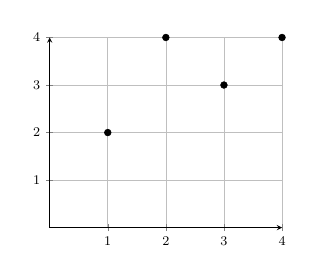
\begin{tikzpicture}[scale=0.6]
    \begin{axis}[
            grid = major,
            xmin=0, xmax=4,
            ymin=0, ymax=4,
            axis lines=center,
            axis on top=true,
            small,
            domain=0:4,
        ]
        \addplot[only marks, color = black, mark = *]
        table[meta=label] {
            x       y       label
            1       2       a
            2       4       a
            3       3       a
            4       4       a
        };
    \end{axis}
    \end{tikzpicture} 
    \caption{polynomial p}
\end{figure}

\noindent
Instead of solving the polynomial, we will start to divide the problem into smaller pieces and solve them one by one. We create a polynomial,\begin{math} \lambda_1, \lambda_2, \lambda_3\end{math} and \begin{math}\lambda_4\end{math}, one for each point from polynomial \textit{p}. These polynomial takes value 1 in one point and 0 in the other points. For example \begin{math} \lambda_1\end{math} takes 1 in 1 and 0 in 2,3 and 4.

\begin{figure}[H]
    \centering
    \captionsetup[subfigure]{labelformat=empty}
    \begin{subfigure}[b]{0.3\textwidth}
        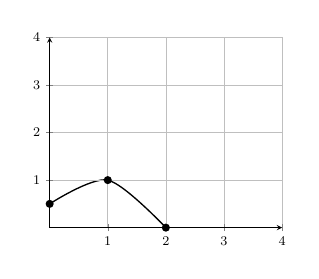
\begin{tikzpicture}[scale=0.6]
        \begin{axis}[
                grid = major,
                xmin=0, xmax=4,
                ymin=0, ymax=4,
                axis lines=center,
                axis on top=true,
                small,
            ]
            \addplot[smooth, thick, color = black, mark = *]
            table[meta=label] {
                x       y       label
                0       0.5     a
                1       1       a
                2       0       a
            };
        \end{axis}
        \end{tikzpicture} 
        \caption{approximately $\lambda_1$}
    \end{subfigure}
    \qquad % <----------------- SPACE BETWEEN PICTURES
    \qquad % <----------------- SPACE BETWEEN PICTURES
    \qquad % <----------------- SPACE BETWEEN PICTURES
    \qquad % <----------------- SPACE BETWEEN PICTURES
    \begin{subfigure}[b]{0.3\textwidth}
        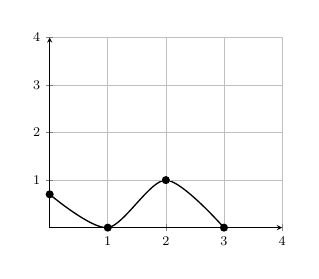
\begin{tikzpicture}[scale=0.6]
        \begin{axis}[
                grid = major,
                xmin=0, xmax=4,
                ymin=0, ymax=4,
                axis lines=center,
                axis on top=true,
                small,
            ]
            \addplot[smooth, thick, color = black, mark = *]
            table[meta=label] {
                x       y       label
                0       0.7     a
                1       0       a
                2       1       a
                3       0       a
            };
        \end{axis}
        \end{tikzpicture} 
        \caption{approximately $\lambda_2$}
    \end{subfigure}
\end{figure}

\noindent
Note that the evaluation in 0 will depend on the secret. For the sake of the drawings it is just an approximately of the point.

\begin{figure}[H]
    \centering
    \captionsetup[subfigure]{labelformat=empty}
    \begin{subfigure}[b]{0.3\textwidth}
        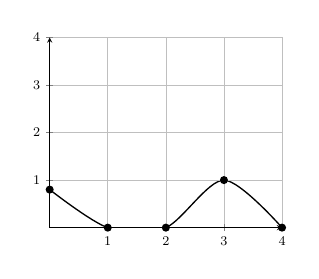
\begin{tikzpicture}[scale=0.6]
        \begin{axis}[
                grid = major,
                xmin=0, xmax=4,
                ymin=0, ymax=4,
                axis lines=center,
                axis on top=true,
                small,
            ]
            \addplot[smooth, thick, color = black, mark = *]
            table[meta=label] {
                x       y       label
                0       0.8     a
                1       0       a
                2       0       a
                3       1       a
                4       0       a
            };
        \end{axis}
        \end{tikzpicture} 
        \caption{approximately $\lambda_3$}
    \end{subfigure}
    \qquad % <----------------- SPACE BETWEEN PICTURES
    \qquad % <----------------- SPACE BETWEEN PICTURES
    \qquad % <----------------- SPACE BETWEEN PICTURES
    \qquad % <----------------- SPACE BETWEEN PICTURES
    \begin{subfigure}[b]{0.3\textwidth}
        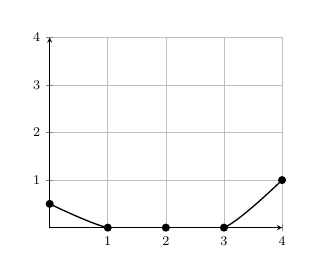
\begin{tikzpicture}[scale=0.6]
        \begin{axis}[
                grid = major,
                xmin=0, xmax=4,
                ymin=0, ymax=4,
                axis lines=center,
                axis on top=true,
                small,
            ]
            \addplot[smooth, thick, color = black, mark = *]
            table[meta=label] {
                x       y       label
                0       0.5     a
                1       0       a
                2       0       a
                3       0       a
                4       1       a
            };           
        \end{axis}
        \end{tikzpicture} 
        \caption{approximately $\lambda_4$}
    \end{subfigure}
\end{figure}

\noindent
To construct the polynomial \begin{math}p\end{math} is to take each polynomials and multiply the corresponding coefficient from \begin{math}p\end{math} and then sum the polynomials together \begin{math}2∙\lambda_1+4∙\lambda_2+3∙\lambda_3+4∙\lambda_4 \end{math}. We started with the \begin{math}\lambda\end{math} polynomial and we ended with four polynomials, which takes value 2,4,3,4 and 0 in the other points. From the sum we see that the value in the first point 2+0+0+0. It is clear this will work in the other points. 

\begin{figure}[H]
    \centering
    \captionsetup[subfigure]{labelformat=empty}
    \begin{subfigure}[b]{0.3\textwidth}
        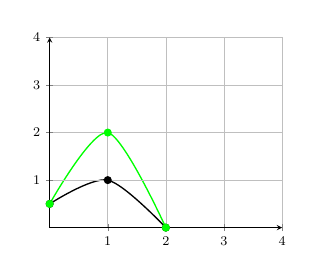
\begin{tikzpicture}[scale=0.6]
        \begin{axis}[
                grid = major,
                xmin=0, xmax=4,
                ymin=0, ymax=4,
                axis lines=center,
                axis on top=true,
                small,
            ]
            \addplot[smooth, thick, color = black, mark = *]
            table[meta=label] {
                x       y       label
                0       0.5     a
                1       1       a
                2       0       a
            };
            \addplot[smooth, thick, color = green, mark = *]
            table[meta=label] {
                x       y       label
                0       0.5     a
                1       2       a
                2       0       a
            };             
        \end{axis}
        \end{tikzpicture} 
        \caption{approximately $\lambda_1$}
    \end{subfigure}
    \qquad % <----------------- SPACE BETWEEN PICTURES
    \qquad % <----------------- SPACE BETWEEN PICTURES
    \qquad % <----------------- SPACE BETWEEN PICTURES
    \qquad % <----------------- SPACE BETWEEN PICTURES
    \begin{subfigure}[b]{0.3\textwidth}
        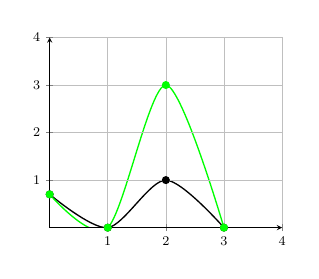
\begin{tikzpicture}[scale=0.6]
        \begin{axis}[
                grid = major,
                xmin=0, xmax=4,
                ymin=0, ymax=4,
                axis lines=center,
                axis on top=true,
                small,
            ]
            \addplot[smooth, thick, color = black, mark = *]
            table[meta=label] {
                x       y       label
                0       0.7     a
                1       0       a
                2       1       a
                3       0       a
            };
            \addplot[smooth, thick, color = green, mark = *]
            table[meta=label] {
                x       y       label
                0       0.7     a
                1       0       a
                2       3       a
                3       0       a
            };             
        \end{axis}
        \end{tikzpicture} 
        \caption{approximately $\lambda_2$}
    \end{subfigure}
\end{figure}

\begin{figure}[H]
    \centering
    \captionsetup[subfigure]{labelformat=empty}
    \begin{subfigure}[b]{0.3\textwidth}
        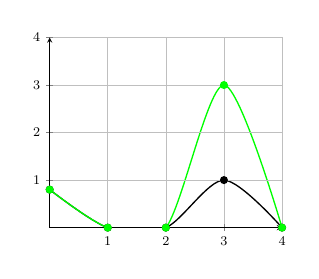
\begin{tikzpicture}[scale=0.6]
        \begin{axis}[
                grid = major,
                xmin=0, xmax=4,
                ymin=0, ymax=4,
                axis lines=center,
                axis on top=true,
                small,
            ]
            \addplot[smooth, thick, color = black, mark = *]
            table[meta=label] {
                x       y       label
                0       0.8     a
                1       0       a
                2       0       a
                3       1       a
                4       0       a
            };
            \addplot[smooth, thick, color = green, mark = *]
            table[meta=label] {
                x       y       label
                0       0.8     a
                1       0       a
                2       0       a
                3       3       a
                4       0       a
            };            
        \end{axis}
        \end{tikzpicture} 
        \caption{approximately $\lambda_3$}
    \end{subfigure}
    \qquad % <----------------- SPACE BETWEEN PICTURES
    \qquad % <----------------- SPACE BETWEEN PICTURES
    \qquad % <----------------- SPACE BETWEEN PICTURES
    \qquad % <----------------- SPACE BETWEEN PICTURES
    \begin{subfigure}[b]{0.3\textwidth}
        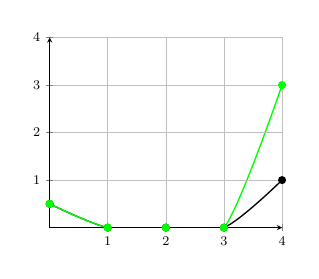
\begin{tikzpicture}[scale=0.6]
        \begin{axis}[
                grid = major,
                xmin=0, xmax=4,
                ymin=0, ymax=4,
                axis lines=center,
                axis on top=true,
                small,
            ]
            \addplot[smooth, thick, color = black, mark = *]
            table[meta=label] {
                x       y       label
                0       0.5     a
                1       0       a
                2       0       a
                3       0       a
                4       1       a
            };
            \addplot[smooth, thick, color = green, mark = *]
            table[meta=label] {
                x       y       label
                0       0.5     a
                1       0       a
                2       0       a
                3       0       a
                4       3       a
            };               
        \end{axis}
        \end{tikzpicture} 
        \caption{approximately $\lambda_4$}
    \end{subfigure}
\end{figure}


\noindent
We will now construct one of the \begin{math}\lambda\end{math}-polynomials by example, by showing it from \begin{math}\lambda_1\end{math} polynomial. 
We have the following points \begin{math}\lambda_1(1)=1, \lambda_1(2)=0, \lambda_1(3)=0 \end{math} and \begin{math} \lambda_1 (4)=0\end{math}. We take the polynomial \begin{math} (x-2)(x-3)(x-4)\end{math}, and we see that if we get correct evaluation in \begin{math}\lambda_1 (2)=0, \lambda_1 (3)=0\end{math} or \begin{math} \lambda_1 (4)=0\end{math}. To get correct evaluation in  \begin{math} \lambda_1 (1)=1\end{math} we divide by \begin{math}-6\end{math} because we see that \begin{math}(1-2)(1-3)(1-4)=-6\end{math} and then we end up with a polynomial \begin{math}\frac{(x-2)(x-3)(x-4)}{(-6)}\end{math} .  The polynomial still satisfies the conditions because when we divide zero with "something" we get zero.  The formula for constructing \begin{math}\lambda_1\end{math} 

\begin{center}
\begin{math} \lambda_1(x)=\prod\limits_{j\in C,j\neq1} \frac{x-j}{1-j} = \frac{x-2}{1-2} \cdot \frac{x-3}{1-3} \cdot \frac{x-4}{1-4}=\frac{(x-2)(x-3)(x-4)}{-6} \end{math}\\
\end{center}

\noindent
\begin{math} \lambda_1\end{math} gives 1 in point 1 and 0 in the other points. What this mean is that in \begin{math} \lambda_1(1)=1\end{math} and all other points  \begin{math}j (2,3,4)\end{math} we have \begin{math} \lambda_1 (j)=0\end{math}. We can construct \begin{math}\lambda_1, \lambda_2, \lambda_3\end{math} and  \begin{math}\lambda_4\end{math} in the same way.

\begin{center}
\begin{math} \lambda_2(x)=\prod\limits_{j\in C,j\neq2} \frac{x-j}{2-j} = \frac{x-1}{2-1} \cdot \frac{x-3}{2-3} \cdot \frac{x-4}{2-4}=\frac{(x-1)(x-3)(x-4)}{-2} \end{math}\\ 

\begin{math} \lambda_3(x)=\prod\limits_{j\in C,j\neq3} \frac{x-j}{3-j} = \frac{x-1}{3-1} \cdot \frac{x-3}{3-2} \cdot \frac{x-4}{3-4}=\frac{(x-1)(x-2)(x-4)}{-2} \end{math}\\ 

\begin{math} \lambda_4(x)=\prod\limits_{j\in C,j\neq4} \frac{x-j}{4-j} = \frac{x-1}{4-1} \cdot \frac{x-3}{4-2} \cdot \frac{x-3}{4-3}=\frac{(x-1)(x-2)(x-3)}{-6} \end{math}\\ 
\end{center}

\noindent
With the knowledge of the evaluation of \begin{math}p(1), p(2), p(3)\end{math} and  \begin{math}p(4)\end{math} we construct the formula for polynomial evaluation in \begin{math}p(0)\end{math}:


\noindent
\begin{infobox}[Applying Lagrange polynomial interpolation for polynomial evaluation in $0$]
We use the formula \begin{math}p(x)=\sum\limits_{i \in C} p(i)\lambda_i(x)\end{math} and we get the evaluation on some polynomial in $0$
\begin{center}
\begin{math}p(0)=p(1)∙\lambda_1+p(2)∙\lambda_2+p(3)∙\lambda_3+p(4)∙\lambda_4=2∙\lambda_1+4∙\lambda_2+3∙\lambda_3+4∙\lambda_4 \end{math}
\end{center}
\label{info:Applying_Lagrange_polynomial_interpolation}
\end{infobox}



\noindent
The idea of constructing the smaller polynomials is that we can reuse them for constructing other polynomials. From the smaller pieces and the evaluation points we can construct the polynomial from Lagrange interpolation. From the secret sharing scheme we know the degree of the polynomial is bounded. Because the voter will share its secret by choosing a random polynomial of the degree at most \textit{t}. That’s a guaranty we have from the scheme. If the degree of $p(x)$ is at most \textit{t} meaning $p(x)\leq t$. Then we need $t+1$ point to reconstruct the $p(x)$. If the degree 1 (line) then we need two points. The parable is where the degree is 2, here we need 3 points to construct
the polynomial.

\begin{figure}[H]
    \centering
    \captionsetup[subfigure]{labelformat=empty}
    \begin{subfigure}[b]{0.3\textwidth}
        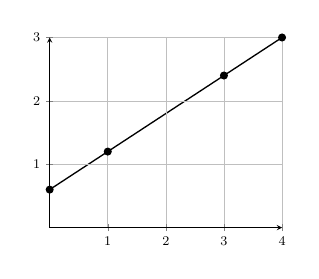
\begin{tikzpicture}[scale=0.6]
        \begin{axis}[
                grid = major,
                xmin=0, xmax=4,
                ymin=0, ymax=3,
                axis lines=center,
                axis on top=true,
                small,
            ]
            \addplot[smooth, thick, color = black, mark = *]
            table[meta=label] {
                x       y       label
                0       0.6     a
                1       1.2     a
                3       2.4     a
                4       3       a
            };
        \end{axis}
        \end{tikzpicture} 
        \caption{polynomial of degree 1}
    \end{subfigure}
    \qquad % <----------------- SPACE BETWEEN PICTURES
    \qquad % <----------------- SPACE BETWEEN PICTURES
    \qquad % <----------------- SPACE BETWEEN PICTURES
    \qquad % <----------------- SPACE BETWEEN PICTURES
    \begin{subfigure}[b]{0.3\textwidth}
        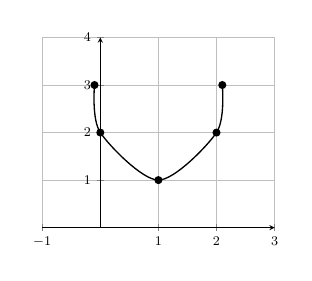
\begin{tikzpicture}[scale=0.6]
        \begin{axis}[
                grid = major,
                xmin=-1, xmax=3,
                ymin=0, ymax=4,
                axis lines=center,
                axis on top=true,
                small,
            ]
            \addplot[smooth, thick, color = black, mark = *]
            table[meta=label] {
                x       y       label
                -0.1    3       a
                0       2       a
                1       1       a
                2       2       a
                2.1     3

            };           
        \end{axis}
        \end{tikzpicture} 
        \caption{polynomial of degree 2}
    \end{subfigure}
\end{figure}


\parahead{In the PVSS protocol} we will use a simplified version of Lagrange interpolation formula. So instead of recovering the polynomium we just recover the evaluation in zero. The following will happen if take the formula \begin{math} \lambda_i(x)=\prod\limits_{j\in C,j\neq i}  \frac{x-j}{i-j} \end{math} and evaluate in zero \begin{math} \lambda_i(0)=\prod\limits_{j\in C,j\neq i}  \frac{0-j}{i-j} = \prod\limits_{j\in C,j\neq i} \frac{j}{j-i} \end{math}. We reduce the formula by evaluating in $0$ and then one can multiply the numerator and denominator by $-1$ and then we get a the above formula.


\noindent
\begin{infobox}[Computing the coefficients for 3 participants]
\begin{math}\lambda_1(0)=\prod\limits_{j\in C,j\neq 1} \frac{2}{2-1}  \cdot  \frac{3}{3-1} =\frac{3}{1} = 3 \end{math}\\
\begin{math}\lambda_2(0)=\prod\limits_{j\in C,j\neq 2} \frac{1}{1-2}  \cdot  \frac{3}{3-2} =\frac{1}{-1} \cdot  \frac{3}{1} =-1 \cdot  3=-3 \end{math}\\
\begin{math}\lambda_3(0)=\prod\limits_{j\in C,j\neq 3} \frac{1}{1-3}  \cdot  \frac{2}{2-3} =\frac{1}{-2} \cdot  \frac{2}{-1} =1 \end{math}\\
\label{info:Computing_the_coefficients}
\end{infobox}

\subsection{Example computation using Shamir Secret Sharing}
We have now explained the basic for secret sharing. This section will show a full concrete computational example on distribution and reconstruction of a secret between 5 participant where we want to tolerate $t=2$ corrupted parties. The computation is computed in $\Z_{11}^*$. The example is that one participant, $p_1$, has a secret, $s=7$ and creates shares to the other participants ($p_2, p_3, p_4, p_5$). Then if $3$ participants combines the shares they will be able to reconstruct the secret. \\

\noindent
First the participant $p_1$ creates a random polynomium, $p(x)$ at degree $t=2$ which is the following polynomium $p(x)=s + a_{1}x+ a_{2}x^2$, where $s=7$ is the secret and $a_{1}=4$ and $a_{2}=1$ is coefficient randomly choosen from $\Z_{11}^*$. The following will show the distribution where $p_1$ create shares to the other parties. In the reconstruction we show how $3$ parties will be able to reconstruct the polynomial and the secret by their shares using Lagrange interpolation.   

\subsubsection{Distribution}
The shares $s_1, s_2, s_3, s_4,s_5$ is computed from $p(x)=7 + 4x+ x^2$ as

\noindent
\begin{alignat*}{4}
s_1&=p(1)&&= 7+4+1 \ &&(mod \ 11) &&=1 \\
s_2&=p(2)&&= 7+8+4 \ &&(mod \ 11) &&=8 \\
s_3&=p(3)&&= 7+12+9 \ &&(mod \ 11) &&=6 \\
s_4&=p(4)&&= 7+16+16 \ &&(mod \ 11) &&=6 \\
s_5&=p(5)&&= 7+20+25 \ &&(mod \ 11) &&=8    
\end{alignat*}


\noindent
Each party now recieve their shares secure. So $p_2= s_2, p_3=s_3, p_4= s_4, p_5= s_5$.

\subsubsection{Reconstruction}
A subset, $3>2$, of participant $p_3, p_4, p_5$ wants to reconstruct the secret by their shares using Lagrange interpolation. First every party computes a polynomial. After that the parties will be able to combine their polynomial and their shares to reconstruct $p(x)$.\\

%------------------------------------------------------------------------------------
\noindent
$p_3$ computes:
%------------------------------------------------------------------------------------


\noindent
\begin{alignat*}{3}
\lambda_3(x)&=\prod\limits_{j\in C,j\neq3} \frac{x-j}{3-j} = \frac{x-4}{3-4} \cdot \frac{x-5}{3-5} =\frac{(x-4)(x-5)}{(3-4)(3-5)}  \\
&= (x^2-9x+20)((3-4)(3-5))^{-1} \ (mod \ 11)
\end{alignat*}

\noindent
The inverse of  $((3-4)(3-5))= 2$ is $6$ since $2 \cdot 6 \ mod \ 11 = 1$. We now have the following polynomial

\noindent
\begin{alignat*}{3}
\lambda_3(x) = (x^2-9x+20)6 \ (mod \ 11) &= (x^2 + 2x+9)6 \ &(mod \ 11) \\
&= 6x^2 + 12x + 54 \ &(mod \ 11) \\
&= 6x^2+x+ 10 \ &(mod \ 11) 
\end{alignat*}

\noindent
We verify the following


\noindent
\begin{alignat*}{6}
\lambda_3(3) &=  6 \cdot 3^2+3+ 10  \ &&(mod \ 11) &&= 67 \ &&(mod \ 11) &&= 1 \\
\lambda_3(4) &=  6 \cdot 4^2+4+ 10  \ &&(mod \ 11) &&= 110 \ &&(mod \ 11) &&= 0 \\
\lambda_3(5) &=  6 \cdot 5^2+5+ 10  \ &&(mod \ 11) &&= 165 \ &&(mod \ 11) &&= 0
\end{alignat*}

%------------------------------------------------------------------------------------
\noindent
$p_4$ computes:
%------------------------------------------------------------------------------------

\noindent
\begin{alignat*}{3}
 \lambda_4(x)&=\prod\limits_{j\in C,j\neq4} \frac{x-j}{4-j} = \frac{x-3}{4-3} \cdot \frac{x-5}{4-5} =\frac{(x-3)(x-5)}{(4-3)(4-5)}\\ 
 &= (x^2-8x+15)((4-3)(4-5))^{-1} \ (mod \ 11)
\end{alignat*}



\noindent
The inverse of  $((4-3)(4-5))= -1$ is $10$ since $-1 \cdot 10 \ (mod \ 11) = 1$. We now have the following polynomial


\noindent
\begin{alignat*}{3}
\lambda_4(x) = (x^2-8x+15)10 \ (mod \ 11) &= (x^2 + 3x+4)10 \ &&(mod \ 11) \\
                                          &= 10x^2 + 8x + 7 \ &&(mod \ 11) 
\end{alignat*}

\noindent
We verify the following

\noindent
\begin{alignat*}{3}
\lambda_4(3) &=  10 \cdot 3^2+24+ 7  \ (mod \ 11) &&= 121 \ (mod \ 11) = 0 \\
\lambda_4(4) &=  10 \cdot 4^2+32+ 7  \ (mod \ 11) &&= 199 \ (mod \ 11) = 1 \\
\lambda_4(5) &=  10 \cdot 5^2+40+ 7  \ (mod \ 11) &&= 297 \ (mod \ 11) = 0 \\
\end{alignat*}




%------------------------------------------------------------------------------------
\noindent
$p_5$ computes:
%------------------------------------------------------------------------------------

\noindent
\begin{alignat*}{3}
 \lambda_5(x)&=\prod\limits_{j\in C,j\neq5} \frac{x-j}{5-j} = \frac{x-3}{5-3} \cdot \frac{x-4}{5-4} =\frac{(x-3)(x-4)}{(5-3)(5-4)} \\
&= (x^2-7x+12)((5-3)(5-4))^{-1} \ (mod \ 11)
\end{alignat*}



\noindent
The inverse of  $((5-3)(5-4))= 2$ is $6$ since $2 \cdot 6 \ mod \ 11 = 1$. We now have the following polynomial

\noindent
\begin{alignat*}{3}
\lambda_5(x)= (x^2-7x+12)6 \ (mod \ 11) &= (x^2 + 4x+1)6 \ &&(mod \ 11) \\
                                        &= 6x^2 + 24x + 6 \ &&(mod \ 11) \\
                                        &= 6x^2 + 2x + 6 \ &&(mod \ 11)
\end{alignat*}

\noindent
We verify the following

\noindent
\begin{alignat*}{6}
\lambda_5(3) &=  6 \cdot 3^2+6+ 6  \ &&(mod \ 11) &&= 66 \ &&(mod \ 11)  &&= 0 \\
\lambda_5(4) &=  6 \cdot 4^2+8+ 6  \ &&(mod \ 11) &&= 110 \ &&(mod \ 11) &&= 0 \\
\lambda_5(5) &=  6 \cdot 5^2+10+6  \ &&(mod \ 11) &&= 166 \ &&(mod \ 11) &&= 1  
\end{alignat*}




\noindent
To construct the polynomial \begin{math}p\end{math} we take each polynomials and multiply by the corresponding shares. More formally we apply \begin{math}p(x)=\sum\limits_{i \in C} p(i)\lambda_i(x)\end{math} to construct the $p(x)$.



\noindent
 \begin{alignat*}{2}
p(x) &= s_3 \lambda_3 (x) + s_4 \lambda_4 (x) + s_5 \lambda_5 (x) &\\
     &= s_3(6x^2+x+ 10) + s_4(10x^2 + 8x + 7)  + s_5(6x^2 + 2x + 6)&\\
     &= (6s_3+10s_4+6s_5)x^2 + (s_3 + 8s_4 + 2s_5)x  + (10s_3 + 7s_4 + 6s_5)&
\end{alignat*} 
   

\noindent
Since the polynomial is of the form $p(x)=s + a_{1}x+ a_{2}x^2$ we have that

\noindent
\begin{alignat*}{2}
s&  = 10s_3 + 7s_4 + 6s_5 \ &&(mod \ 11)  \\
a_1&= s_3 + 8s_4 + 2s_5\ &&(mod \ 11) \\
a_2&= 6s_3+10s_4+6s_5\ &&(mod \ 11) 
\end{alignat*} 

\noindent
We can now replace the variables with shares $s_3=6, s_4=6, s_5=8$

\noindent
\begin{alignat*}{6}
s&  = 10 \cdot 6 + 7 \cdot 6 + 6 \cdot 8 \ &&(mod \ 11)  &&= 150  \ &&(mod \ 11) &&= 7\\
a_1&= 6 + 8 \cdot 6 + 2 \cdot 8 \ &&(mod \ 11) &&= 70  \ &&(mod \ 11) &&= 4\\
a_2&= 6 \cdot 6 +10 \cdot 6+ 6 \cdot 8 \ &&(mod \ 11) &&= 144  \ &&(mod \ 11) &&= 1
\end{alignat*}

\noindent
The reconstruction gives us the final polynomial $p(x)=7 + 4x+ x^2$ and thereby the secret value $7$.


\subsection{Verifiable Secret Sharing (VSS)}
Where the basic model of secret sharing assumes that every participants involved is honest, the VSS requires its participants to prove so. The objective of the VSS is to resisted malicious participants which are defined as \cite{Schoenmakers1999}

\begin{itemize}
    \item Dealer is sending incorrect shares to some or all participants in the distribution phase
    \item Participants is submitting incorrect shares during the reconstruction phase
\end{itemize}

\noindent 
By requiring proof of correctness of the shares, from the participants, in the distribution and the reconstruction phase, the VSS model solves the problem of malicious participants. These proofs is constructed in such a way that only the participants is able to construct and verify the proofs. Where it is a logical requirement that only the participants is able to construct the proofs, it is a different story with the verification. In fact in most case it would be ideal if anybody could validate the proofs. 


\subsection{Public Verifiable Secret Sharing (PVSS)}
In a PVSS schemes it is required that, not only the participants but anybody, is able to validate the shares. It is therefore not assumed that there are private channels between the participants. All communication in PVSS schemes  is done over authenticated public channels using public key encryption, which also means that the secret is only computationally hidden. A common structure for the PVSS protocols is as follows.

\begin{description}
    \item[Initialization] Each participants registers itself and must have a public key.  
    
    \item[Distribution] consists of a distribution and a verification phase
    
    \begin{enumerate}
        \item \textit{Distribution of the shares}
        \begin{enumerate}
            \item \textit{Dealer creates shares}
            \item \textit{Dealer publishes encrypted shares}    
            \item \textit{Dealer publishes a $proof_D$}   
        \end{enumerate}
        \item \textit{Verification of the shares} 
        \begin{enumerate}
            \item \textit{Anybody who knows the public key can verifier the shares}
            \item \textit{If the verification on $proof_D$ fails the dealer fails and the protocol is aborted}  
        \end{enumerate}
    \end{enumerate}
    
    
    \item[Reconstruction] consists of a decryption phase and pooling the shares phase    
        
    \begin{enumerate}
        \item \textit{Decryption of the shares}
         \begin{enumerate}
            \item \textit{The participants decrypt their shares}
            \item \textit{The participants publishes a $proof_{p_{i}}$}  
        \end{enumerate}
        \item \textit{Pooling the shares}  
        \begin{enumerate}
            \item \textit{$proof_{p_{i}}$ are used to exclude dishonest participants}
            \item \textit{Reconstruction of the secret by any qualified set of participants}  
        \end{enumerate}
    \end{enumerate}        

\end{description}

%------------------------------------------------------------------------------------
\subsection{Homomorphic Secret Sharing}
%------------------------------------------------------------------------------------
A homomorphism is a transformation from one algebraic structure into another of the same type so that the structure is preserved. Importantly, this means that for every kind of manipulation of the original data, there is a corresponding manipulation of the transformed data.\\

\noindent 
A homomorphic encryption scheme is a crypto system that allows computations to be performed on data without decrypting it. It is an encrypting scheme which allows computations to be carried out on ciphertext, thus generating an encrypted result which, when decrypted, matches the result of operations performed on the plaintext.

\parahead{Homomorphic Secret Sharing} is a type of secret sharing algorithm in which the secret is encrypted via homomorphic encryption. In the PVSS scheme we use this property that one can sum the shares which are equal to the sum of the secrets.


    
    
 \clearpage
%***************************************************************
%               Part 5: The Protocol
%***************************************************************  
\chapter{Electronic voting protocol}
    In this section we look at the electronic voting protocol described in \cite{Schoenmakers1999}. The protocol is based on the PVSS protocol describe in the same article. We will only be describing the electronic voting protocol but as doing so, the relevant elements from the PVSS protocol will taking into the description. For the rest of this chapter we will be referring to the electronic voting protocol, as simply the protocol, unless specified otherwise. \\

\noindent
Giving the complexity of the protocol we divided this description into three parts. In the first part we will be describing the protocol as simple as possible, living out mathematical justification and proofs. In second part we will be looking at the mathematical justification, describing this in the same order as in the first part. and finally we will be look though the proofs in the last part. 


\section{The protocol}


\noindent
In the PVSS protocol there will be a group of voters where each voter votes $0$ or $1$. The result of the votation is the sum of the votes. The votes are going to be counted by group of talliers where no tallier knows the individual votes, even if a certain group of talliers are corrupted by the same adversary. There will be a bullutin board where voters/talliers put their public information. This allows the correctness of the voter and tallier to be publicly verified.\\

\noindent
The PVSS protocol is a protocol which can handle a large set of secret data but it can also handle a small set data. This means that one of its applications is a  electronic voting system where the secret may differ from 0 or 1. The PVSS protocol differs from standard MPC protocol in which the shares are made public and verifiable.\\\\
This section will start by explaining our requirements for our implementation and after that we will explain the protocol. The main part will be the Ballot casting where the voter distribute their shares and the Tallying where the tallier computes and reconstructs the votes. The last part will go in depth with the mathematical proofs. \\







\noindent
\textbf{Short overview of the protocol}

\noindent
\begin{enumerate}
    \item \textbf{Initialization}
        \begin{enumerate}
        \item Each voter signs it name on the bulletin board.
        \item Each tallier generates a private and a public key.
        \item Each tallier registries their public keys on the bulletin board.
        \item The system generates and publishes system parameters and sets security requirements.
        \end{enumerate}
    \item \textbf{Ballot casting}
    \begin{enumerate}
        \item Each voter votes $1$ or $0$
        \item Each voter generates a random secret.
        \item Each voter creates shares of the secret to each tallier and encrypts it with the corresponding public key of the tallier. Each voter supply this secret share with evidence of its consistency with a $DLEQ$ proof.
        \item Each voter supply evidence for a valid vote with $PROOF_U$.
    \end{enumerate}
    \item \textbf{Tallying}
    \begin{enumerate}
        \item At least $t-1$ tallier accumulates and decrypts their shares.
        \item One authority completes the final computation of the total votes.
    \end{enumerate}
\end{enumerate}


\noindent
In the following we will describe the central parts of the protocol. We will use terms as Bulletin board which is keen of public board where all the public values gets posted. Tallying is in this context those who counts the votes.\\


\noindent
For efficiency we will limit the computation of the votes to a finite number of talliers. There are \textit{m} voters and \textit{n} talliers. 
%--------------------------------------------------------------------------
\subsection{Initialization}
%--------------------------------------------------------------------------

\noindent
\textbf{The bulletin board generates all system parameters. The public elements $f$ and $F$ and a security parameter $t$.}


\begin{alignat*}{2}
f \ &\in_R \{1,...,2q\} \rightarrow g &&= f^2 \ mod\ 2q+1 \wedge g\neq1\\
F \ &\in_R \{1,...,2q\}\rightarrow G &&= F^2 \ mod\ 2q+1 \wedge G\neq1\\
t &\in_R \Z_q^* &&= \{1,2,3,...,q-1\} 
\end{alignat*}

\noindent
\textbf{The tallier generates a private, $x_i$ and a public keys $y_i$.}
\begin{alignat*}{2}
x_{i} \in_R \Z_q^* &= \{1,2,3,...,q-1\}\\
y_i=G^{x_i} ,\ i &=\{1,2,3,...., n \}
\end{alignat*}


%--------------------------------------------------------------------------
\subsection{Ballot casting}
%--------------------------------------------------------------------------
The  Ballot casting consists of \textit{distribution of the shares} and \textit{verification of the shares}.\\

\noindent
First the voter either votes "no" or "yes" corresponding to 0 or 1. The voter select a random secret value \begin{math}s \end{math}. The PVSS protocol is then used to distribute shares which contain a combination of the random secret and the vote. Every voter will construct a random polynomial at degree $t$ and then evaluate the shares  to each of the talliers.\\


\noindent
\textbf{The voter creates his vote, a random value and a random polynomial of degree at most $t$ and computes the shares.}

\begin{flalign*}
Vote &: v\in\{0,1\} & \\
Random \ value  &: s\in_R \Z_q &\\
SSS &:  p(x)=s+\alpha_1x^1+\alpha_2x^2+,...,+\alpha_{t-1}x^{t-1}, \ \alpha_j\in_R \Z_q &\\
Secret \ Shares &:  p(0)=s,\ p(1),\ p(2),...,\ p(n)
\end{flalign*}

\noindent
\textbf{The voter distributes the encrypted share and creates a $PROOF_U$ and a $DLEQ$ proof.}\\
The \begin{math}p(i)\end{math} is the share where we use Shamir Secret Sharing. The \begin{math}\alpha_j\end{math} is all the coefficients besides that $\alpha_0$ is set to the $s$ value. The shares are going to be encrypted using the talliers public key $y_i^{p(i)}$. The following gets publish to the bulleting board

\begin{alignat*}{2}
Y_i&=y_i^{p(i)} ,1\leq i\leq n \ (Encryption \ of \ the \ share) \\ 
C_j&=g^{\alpha_j},\ j =\{0,1,2,3,....,t-1 \}, \ where \ \alpha_0 = s  \\ 
X_i&=\prod\limits_{j=0}^{t-1} C_j^{i^j} =g^{p(i)}, 1\leq i\leq n\\
U&=G^{s+v}
\end{alignat*}

\noindent
Besides above computed parameters a  $PROOF_U$ proof and a $DLEQ$ proof are computed. \\

\noindent
With $DLEQ$ we prove that the exponent are equal \begin{math}X_i=g^{p(i)}  \land Y_i=y_i^{p(i)} \end{math} without revealing \begin{math}{p(i)} \end{math}. We will present an interactive and a non-interactive proof of the $DLEQ$ between the voter and the verifier.\\

\noindent
With \begin{math} PROOF_U \end{math} the voter proofs "consistency" and that the vote is either 1 or 0. Note that the construction of $Y_i$ is a hard problem to solve as we discussed in the discrete logarithm section.




%--------------------------------------------------------------------------
\subsection{Tallying}
%--------------------------------------------------------------------------
Tallying is the process of counting the votes. Here the tallier uses their private keys to collectively compute the final tally, based on the valid ballots.\\



\noindent
\textbf{The tallier decrypts the shares and publishes a $DLEQ$ proof}\\
The homomorphic secret sharing property ensures that each tallier will  be able to multiply the shares and then decrypt. Let $Y_{ij}$ be the value $Y_i$ computed by the j-th voter as described in the previous section. This means concrete that the \textit{i} is referring to tallier 1, tallier  2 and tallier 3 etc. and \textit{j} is referring to voter 1, voter 2 and voter 3 etc.

\begin{alignat*}{2}
Y_i^*=(\prod\limits_{j=1}^{m} Y_{ij}) \ (mod\ 2 \cdot q+1) =y_i^{\sum\limits_{j=1}^m p_j(i)}
\end{alignat*}


\noindent
Following can be reduced by using the talliers private key. Note that we are raising to the multiplicative inverse of the private key in  \textit{q}. The $p_j$ is the polynomium $p$ used by the j-th voter.


\begin{alignat*}{2}
y_i^{\sum\limits_{j=1}^m p_j(i)}=(G^{x_i})^{\sum\limits_{j=1}^m p_j(i)} = G^{x_i \sum\limits_{j=1}^m p_j(i)}= (G^{x_i \sum\limits_{j=1}^m p_j(i)})^{\frac{1}{\mathbf{x_i}}}= G^{ \sum\limits_{j=1}^m p_j(i)}
\end{alignat*}


\noindent
Note that besides decrypting the shares the tallier will publish a $DLEQ$ proof which shows that the decrypting was done correct. See figure \ref{fig:DLEQ_by_talliers} of the $DLEQ$ proof. Also note that we computing the inverse of the key $x_i$. To compute the inverse we will use Extended Euclidean algorithm.\\


\noindent
\textbf{A master authority applies Lagrange interpolation}\\
One can now use lambda, which is computed from the  Lagrange interpolation formular, \begin{math} \lambda_j \end{math} and multiply these values which will be the same as the sum of the exponents. See figure \ref{info:Computing_the_coefficients} \\

\noindent
The \begin{math}p_j(0) \end{math} correspond to the sum of the secret values of \textit{s} for the voters. This \begin{math}p_j(0)\end{math} corresponds to the evaluation of \begin{math}h(0)\end{math}. See figure  \ref{info:Applying_Lagrange_polynomial_interpolation}


\begin{alignat*}{2}
(Y_1^*)^{\lambda_1  \cdot  \ (mod \ q)}  \cdot  (Y_2^*)^{\lambda_2 \ (mod \ q)}  \cdot  (Y_n^*)^{\lambda_n \ (mod \ q)} \ (mod \ 2 \cdot q+1)
\end{alignat*}


\noindent
We can substitute the $Y^*$ with $G$. The final result in the exponents is a evaluation in some polynomium in $0$ which corresponds to the sum of all random values $s$.

\begin{alignat*}{2}
&=G^{ \sum\limits_{j=1}^m \lambda_j p_j(1)} \cdot G^{ \sum\limits_{j=1}^m \lambda_j p_j(2)} \cdot...\cdot G^{ \sum\limits_{j=1}^m \lambda_j p_j(n)}\\
&=G^{ \sum\limits_{j=1}^m \lambda_j p_j(1) +  \sum\limits_{j=1}^m \lambda_j p_j(2) +...+  \sum\limits_{j=1}^m \lambda_j p_j(n)}\\
&=G^{ \sum\limits_{j=1}^m (\lambda_j p_j(1)+\lambda_j p_j(2)+,...,+\lambda_{j}p_j(n))} = G^{ \sum\limits_{j=1}^m p_j(0)}= G^{ \sum\limits_{j=1}^m s_j}
\end{alignat*}


\noindent
\textbf{A master authority computes the votes}\\
The last step is to isolate the votes and then compute the final result. By combining \begin{math}U_j \end{math} we obtain the following.

\begin{alignat*}{2}
(\prod\limits_{j=1}^{m} U_{j}) \ (mod \ 2 \cdot q+1)=  G^{ \sum\limits_{j=1}^m s_j +v_j}
\end{alignat*}

\noindent
By dividing with $G^{ \sum\limits_{j=1}^m s_j}$ we isolate \textit{v}

\begin{alignat*}{2}
\frac{G^{ \sum\limits_{j=1}^m s_j +v_j}}{{ G^{ \sum\limits_{j=1}^m s_j} }} =G^{ \sum\limits_{j=1}^m s_j +v_j -\sum\limits_{j=1}^m s_j} = G^{ \sum\limits_{j=1}^m v_j}
\end{alignat*}

\noindent
To solve the computing of the votes one can compute \begin{math}G^0, G^1, G^3,..., G^{v_j} \end{math} by exhaustive search. A more efficient algorithm is to use Baby-step giant-step algorithm. 

%--------------------------------------------------------------------------
\section{Protocol details}
%--------------------------------------------------------------------------

\subsection{Initialization}
\noindent
\textbf{Strong prime} In our implementation we will pick a prime, \begin{math}q\end{math}, so we avoid doing the gcd computation. The protocol states that we have to compute in a group of order q. This means that when we are doing operations in the exponent this property should be satisfied \begin{math}g^q=1\end{math} where \begin{math}q\end{math} is prime. If we are doing \begin{math}mod \ q \end{math} in the exponent we have \begin{math}g^q=g^0\end{math}. The reason for doing operation in the exponent \begin{math}mod \ q\end{math} is because we are using Sharmir secret sharing which require a finite field.\\

\noindent
One can see that given a generator $g=2 $ and a prime $q=5$, then \begin{math}2^5 \ mod \ 5 = 32 \ mod \ 5 = 2\end{math}. For this to be true, we take the square of numbers modulo a prime in this form \begin{math}2q+1\end{math}. This is also called a strong prime. By using this mathematical structure this property holds. We can choose \begin{math}b=a^2\end{math}. Then we see the property holds \begin{math}b^{q} = 1 \ mod \ 2q+1\end{math}. Using the same values as before, it is clear that \begin{math}(2^2)^5 \ mod \ 11 = 1024 \ mod \ 11 = 1\end{math}. Fermat little theorem states that \begin{math}b^{q-1} \ mod \ q = 1\end{math} where \begin{math}q\end{math} is prime. So we know if we pick our \begin{math}q\end{math} and \begin{math}b\end{math} (as a square)  in this form \begin{math}(a^{2})^{q+1-1} \ mod \ 2q+1 =1 =  a^{2q} \ mod \ 2q+1 =1\end{math} the property holds.

\subsection{Ballot casting}
An example for clarification on the computations of \begin{math}X_i\end{math}. The following is computation of the $X_i$ to tallier 1 ($X_1$), tallier 2 ($X_2$) and tallier 3 ($X_3$).

\begin{alignat*}{3}
X_1 &=\prod\limits_{j=0}^{t-1} C_j^{i^j} &&= C_0^{1^0}  \cdot  C_1^{1^1}  \cdot  C_2^{1^2}\\
X_2 &=\prod\limits_{j=0}^{t-1} C_j^{i^j} &&= C_0^{2^0}  \cdot  C_1^{2^1}  \cdot  C_2^{2^2}\\
X_3 &=\prod\limits_{j=0}^{t-1} C_j^{i^j} &&= C_0^{3^0}  \cdot  C_1^{3^1}  \cdot  C_2^{3^2}
\end{alignat*}




\subsection{Tallying}
An example on the multiplication of the $Y_{ij}$

\begin{alignat*}{4}
Voter \ 1&: Y_{1,1}&&=y_{1,1}^{p_1(1)},Y_{2,1}&&=y_{2,1}^{p_2(2)} ,.., Y_{n,1}&&=y_n^{p_n(n)}\\
Voter \ 2&: Y_{1,2}&&=y_{1,2}^{p_1(1)},Y_{2,2}&&=y_{2,2}^{p_2(2)} ,.., Y_{n,2}&&=y_n^{p_n(n)}\\
Voter \ \textit{m}&: Y_{1,m}&&=y_{1,m}^{p_1(1)} , Y_{2,m}&&=y_{2,m}^{p_2(2)} ,.., Y_{n,m}&&=y_n^{p_n(n)}
\end{alignat*}


\noindent
An example on $Y_i^*$. Each tallier can publish the following. Note that every talliers exponent is the evaluation in some point in a given polynomium \begin{math}h(1), h(2),..., h(n) \end{math}.
\begin{center}
Tallier 1 publish: \begin{math}Y_1^* = G^{ \sum\limits_{j=1}^m p_j(1)}   \end{math}\\
Tallier 2 publish: \begin{math}Y_2^* = G^{ \sum\limits_{j=1}^m p_j(2)}   \end{math}\\
Tallier \textit{n} publish: \begin{math}Y_n^* = G^{ \sum\limits_{j=1}^m p_j(n)}  \end{math}\\
\end{center}



%--------------------------------------------------------------------------
\section{Proofs}
%--------------------------------------------------------------------------
In this section we will elaborate the mathematical justification of the interactive- and non interactive $DLEQ$ and the $PROOF_U$. 

%----------------------------------------------------------------------
\subsection{DLEQ interactive proof between voters and verifier} \label{proofs:dleq_voter_verifier}
%----------------------------------------------------------------------
DLEQ stands for discrete logarithm equality. It proofs that the exponent are equal \begin{math}X_i=g^{p(i)}  \land Y_i=y_i^{p(i)} \end{math} without revealing \begin{math}{p(i)} \end{math} and if the prover was honest, then it should be the case that we get the same computed values in the end meaning $a_1 = g^w= g^r \cdot X_i^C$ and $a_2= y_i^w = y_i^r \cdot Y_i^C$. We will present the protocol and after that we will give concrete examples. Last we will describe the mathematical justification.\\

\noindent
The verification of the shares in the interactive proof happens by the following  interaction between the prover and the verifier.


\begin{figure}[H]
    \centering        
    
    $
    \begin{array}{l}
    \hline                      \
    \textbf{DLEQ protocol}      \\
    \hline                      \
    Public:  g,X_i,y_i,Y_i \ where \ X_i = g^{x_i} \land Y_i=y_i^{x_i}     \\
    \\
	\begin{array}{L{2cm}ccc}
        & \text{\textsf{Prover}} & & \text{\textsf{Verifier}} \\
        \hline
        Step \ 1 & w\in_R \Z_q & & \\
        & a_1=g^w     & & \\
        & a_2=y_i^w   & \xrightarrow{\hspace{1em}a_1, \ a_2\hspace{1em}} & \\
        Step \ 2 & & & C\in_R \Z_q \\
        & & \xleftarrow{\hspace{2em}C\hspace{2em}} & \\
        Step \ 3 & r=w-p(i)  \cdot  C    & & \\
        Step \ 4 & & \xrightarrow{\hspace{2em}r\hspace{2em}} & \begin{array}{c}
        checks \ if: \\      
        a_1 = g^r \cdot X_i^C \\ 
        a_2=y_i^r \cdot Y_i^C
        \end{array} \\
        \hline
    \end{array}
    \end{array}
    $    
    \caption{DLEQ interactive}
	\label{fig:DLEQ_interactive}
\end{figure}
	


\noindent
Note that the verifier sends a challenge \textit{C}, after the prover has computed \begin{math}a_1\end{math} and  \begin{math}a_2\end{math}. The check only passes if the prover used the same exponents. The proof shows that there exist some element \begin{math} \alpha\end{math} such that \begin{math}g^\alpha = X_i \ \land \ y_i^\alpha=Y_i \end{math}. In the following there is an argument why $DLEQ$ works through Zero knowledge proof.\\ 



\noindent
\textbf{Correctness for $DLEQ$}\\
Correctness means if the prover is honest and the statement is true, then the honest verifier always accept. Correctness is shown by verifying the $a_1=g^w \stackrel{?}{=} g^r \cdot X_i^C$ and $a_2=y_i^w \stackrel{?}{=} y_i^r \cdot Y_i^C$ are well constructed. Correctness for $a_1$ is shown by the following.



\begin{alignat*}{3}
a_1 &= g^r \cdot X_i^C \\
&= g^r \cdot (g^{p(i)})^C \\
&= g^r \cdot g^{p(i) \cdot C}\\
&=g^{r+p(i) \cdot C}      \\
&= g^{w - p(i) \cdot C + p(i) \cdot C} &= g^w
\end{alignat*}


\noindent
Correctness for $a_2$ is shown by the following.


\begin{alignat*}{3}
a_2 &= y_i^r \cdot Y_i^C\\
&= y_i^r \cdot (y^{p(i)})^C \\
&= y_i^r \cdot y^{p(i) \cdot C}\\
&=y_i^{r+p(i) \cdot C}      \\
&= y_i^{w - p(i) \cdot C + p(i) \cdot C} &= y_i^w
\end{alignat*}



\noindent
\textbf{Example on $DLEQ$ and why we need a random challenge}\\
We will show a concrete example why we need a challenge and it needs to be random. If the challenge is already is known by the prover for example  assume say it is 1, then the prover can "prepare" and cheat with a wrong statement. 


\begin{enumerate}
    \item The prover sends \begin{math}a_1=g^6 \ \land\ a_2=y_i^7 \ \land \ X_i=g^2 \ \land \ Y_i=y_i^3 \end{math} to verifier.
    \item The verifier creates a challenge \begin{math}C=1 \end{math} to prover.
    \item The prover computes \begin{math}r=w-p(i)  \cdot  C = 6-2  \cdot  1= 4\end{math} and sends $r$ to verifier.
    \item The verifier knows the following  \begin{math}a_1=g^4  \cdot  X_i \ \land \ a_2=y_i^4  \cdot  Y_i \end{math} and now he verifies:
    \begin{enumerate}        
        \item The verifier checks if:  \begin{math}a_1 = g^4 \cdot X_i^C = g^4 \cdot g^{2 \cdot 1} = g^6\end{math}
        \item The verifier checks if:  \begin{math} a_2=y_i^4  \cdot  Y_i^C = y_i^4  \cdot  y_i^{3 \cdot 1}= y_i^7 \end{math}
    \end{enumerate}
\end{enumerate}


\noindent
One can see that both checks passes in this example despite that the prover is dishonest. This shows that if there is no random challenge there wouldnt be soundness because the prover could cheat.\\

\noindent
\textbf{Example on $DLEQ$ with a random challenge which satisfies soundness}\\
Next example shows the verification with a random challenge.

\begin{enumerate}
    \item The prover sends \begin{math}a_1=g^6 \ \land\ a_2=y_i^7 \ \land \ X_i=g^2 \ \land \ Y_i=y_i^3 \end{math} to verifier.
    \item The verifier creates a challenge \begin{math}C=9\ (mod \ 5) \end{math} to prover.
    \item The prover computes \begin{math}r=w-p(i)  \cdot  C = 6-2  \cdot  4 \ (mod \ 5)= 3\end{math} and sends $r$ to verifier.
    \item The verifier knows the following  \begin{math}a_1=g^3  \cdot  X_i \ \land \ a_2=y_i^3  \cdot  Y_i \end{math} and now he verifies:
    \begin{enumerate}        
        \item The verifier checks if: \begin{math}a_1 = g^3 \cdot X_i^C = g^3 \cdot g^{2 \cdot 4} = g^3  \cdot  g^3 = g^6= g^1= g\end{math}
        \item The verifier checks if: \begin{math} a_2=y_i^3  \cdot  Y_i^C = y_i^3  \cdot  y_i^{3 \cdot 4}= y_i^3  \cdot  y_i^{1 \cdot 2}= y_i^3  \cdot  y_i^2= y^5=y^0= 1 \end{math}
    \end{enumerate}
\end{enumerate}

\noindent
Note that soundness is full filled because the check doesn't pass because $a_1=g^6$ is different from $a_1=g$ and $a_2=y_i^7$ is different from $ a_2=y_i^0$. Recall that soundness is if the statement is false then it should fail with overwhelming probability.\\

\noindent
\textbf{The mathematical justification for soundness}\\
In the following we are showing that a prover will fail with overwhelming probability if he is dishonest which satisfies soundness. Since the verifier doesent know that if the first step \begin{math}X_i=g^{p(i)}  \land Y_i=y_i^{p(i)} \end{math} has been computed correctly we denote these exponents by \begin{math}a_1=g^w\end{math}    and \begin{math}a_2=y_i^{w^{'}}\end{math} and \begin{math}X_i=g^{m_i}\end{math}    and \begin{math}Y_i=y_i^{m_i^{'}}\end{math}. We know \begin{math} a_1= g^w \end{math} is equal to \begin{math}g^r  \cdot  X_i^C=g^r \cdot g^{m_i \cdot C} = g^{r+m_i \cdot C}\end{math} and \begin{math} a_2= y_i^{w^{'}}\end{math} is equal to \begin{math}y_i^r  \cdot  Y_i^C=y_i^r \cdot y_i^{m_i^{'} \cdot C} = y_i^{r+m_i^{'} \cdot C}\end{math}. Based on this we can now write two inequalities. In order for these inequalities to be true we can rewrite.

\begin{alignat*}{5}
 a_1 &= g^w &&= g^r  \cdot  X_i^C &&=g^r \cdot g^{m_i \cdot C} &&= g^{r+m_i \cdot C}\\
 a_2 &= y_i^{w^{'}} &&= y_i^r  \cdot  Y_i^C &&=y_i^r \cdot y_i^{m_i^{'} \cdot C} &&= y_i^{r+m_i^{'} \cdot C}
\end{alignat*}

\noindent
We can now write two inequalities

\begin{alignat*}{5}
 w &= r+m_i  \cdot  C\ (mod\ q) &&\implies r &&= w-m_i \cdot C\ (mod\ q)\\
 w^{'} &= r+m_i^{'}  \cdot  C\ (mod\ q) &&\implies r &&= w^{'}-m_i^{'}  \cdot  C\ (mod\ q)
\end{alignat*}
\noindent
These two inequalities has to be equal, therefor we can rewrite

\begin{alignat*}{5}
w-m_i \cdot C = w^i-m_i^{'}\ (mod\ q) \implies (w-w^i)-(m_i - m_i^{'})  \cdot  C = 0 \ (mod\ q) 
\end{alignat*}


\noindent
The prover has to be honest if this equation must be true. It is overwhelming unlikely that, if the prover has been dishonest, where $m_i \neq m_{i^{'}}$, that he will succeed. Since the $C$ is known afterwards the construction of $w$ and $w^{'}$ the probability will be \begin{math} \frac{1}{q}\end{math} for a convincing the verifier. Since the $q$ is a large number then the probability is for the dishonest prover to succeed.\\


\noindent
\textbf{Zero knowledge}\\
The zero knowledge in this context means that the verifier doesn't learn anything about the $p(i)$. One way to argue zero knowledge is by showing that the values sent in the protocol doesn't depend on the $p(i)$. So if one can construct the values $a_1, \ a_2, \ r$  without knowing  $p(i)$  shows that they do not depend on $p(i)$ and we thereby do not learn anything about $p(i)$. One way of doing this is though experiment where on can change the order of the protocol. In is out of this thesis scope to go further depth on this subject.\\

%----------------------------------------------------------------------
\subsection{DLEQ non-interactive proof between voters and verifier}
%----------------------------------------------------------------------
Here we present how one can turn an interactive proof to a non interactive proof. This is also known as the Fiat Shamir where we are transforming a interactive proof into a non interactive proof (signature scheme). Instead of the verifier computes a challenge, the prover computes the challenge as a random function (hash).  We will present two ways off doing this transformation, a non optimized and a optimized version. Last we will describe an example on how this can be done.\\


\parahead{The prover computes} \begin{math}a_1=g^w \ (mod\ q)  \land a_2=y_i^w \ (mod\ q),  w\in_R \Z_q \end{math}. Then the prover computes the hash \begin{math}C=H(X_i,Y_i,a_1,a_2) \end{math}. Then the prover computes  \begin{math}r=w-p(i)  \cdot  C \ (mod\ q)\end{math}. Last the prover publish \begin{math}a_1, a_2,r,C\end{math}. \\

\noindent
\parahead{The verifier computes} the following computations \begin{math}a_1 = g^r \cdot X_i^C  \ (mod\ q)\end{math} and \begin{math} a_2=y_i^r  \cdot  Y_i^C \ (mod\ q)\end{math} and \begin{math}C=H(X_i,Y_i,a_1,a_2)\end{math}.


\begin{figure}[H]
    \centering        
    
    $
    \begin{array}{l}
    \hline                      \
    \textbf{DLEQ protocol}      \\
    \hline                      \
    Public:  g,X_i,y_i,Y_i   \ where \ X_i = g^{x_i} \land Y_i=y_i^{x_i}
    \\
	\begin{array}{L{1.1cm}lcl}
        & \text{\textsf{Prover}} & & \text{\textsf{Verifier}} \\
        \hline
        Step \ 1    &           \begin{array}{l}
                                    w\in_R \Z_q             \\ 
                                    a_1=g^w \ (mod\ q)      \\ 
                                    a_2=y_i^w \ (mod\ q)    \\
                                    C=H(X_i,Y_i,a_1,a_2)    \\
                                    r=w-p(i)  \cdot  C \ (mod\ q)
                                \end{array}     &               & \\
                    &                   &               & \\
        Step \ 2    &                   &               \xrightarrow{\hspace{0.4em}a_1 , a_2 , r , C\hspace{0.4em}} & \begin{array}{l}
            checks \ if: \\      
            a_1 = g^r \cdot X_i^C \\ 
            a_2=y_i^r \cdot Y_i^C \\
            C=H(X_i,Y_i,a_1,a_2)
        \end{array} \\
        \hline
    \end{array}
    \end{array}
    $    
    \caption{DLEQ non interactive}
	\label{fig:DLEQ_1}
\end{figure}


\noindent
Note in above that there is no interaction between the prover and the verifier. \\

\noindent 
\textbf{DLEQ optimized}\\
In the following we will show how one can improve the amount of computation of the challenge \textit{C}. Instead of computing the challenge \textit{n} times, one can compute it once and reuse the challenge.

\begin{enumerate}
    \item The prover publish  \begin{math}a_{1,i}=g^{w_i} \ (mod\ q)  \land a_{2,i}=y_i^{w_i} \ (mod\ q)\end{math}  for  \begin{math} 1\leq i \leq n, \ w_i\in_R \Z_q \end{math}.
    \item The prover computes the hash \begin{math}C=H(X_i,Y_i,...,X_n,Y_n,a_{1,1},a_{2,1},\\a_{1,2},a_{2,2},...,a_{1,n},a_{2,n})\end{math}.
    \item The prover computes \begin{math}r_i\end{math}:  \begin{math}r_i=w_i-p(i)  \cdot  C \ (mod\ q)\end{math} and publish \begin{math}r_i,C\end{math}.
    \item The verification contains of the following computation:
    \begin{enumerate}        
        \item The verifier checks if:   \begin{math}a_{1,i} = g^{r,i} \cdot X_i^C \ (mod\ q) \end{math}
        \item The verifier checks if:  \begin{math} a_{2,i}=y_i^{r_{i}}  \cdot  Y_i^C \ (mod\ q)\end{math}
         \item The verifier checks if:  $C=H(X_i,Y_i,...,X_n,Y_n,a_{1,1},a_{2,1},$\\
$a_{1,2},a_{2,2},...,a_{1,n},a_{2,n})$
    \end{enumerate}
\end{enumerate}

\noindent 
\textbf{DLEQ computation for 3 voters}\\
Hence the hash contains all the  \begin{math}a_i \end{math} the prover will compute this proof once for all  \begin{math}p(i) \end{math} which improve efficiency. This means that if there are 3 voters, then the above computation has to be done 3 times for every tallier, but same hash can be computed once for every tallier. 



\begin{enumerate}
    \item The prover publish $a_{1,1},a_{2,1},a_{1,2},a_{2,2},a_{1,3},a_{2,3}$.
    \item The prover publish $C,r_1,r_2,r_3$.
    \item The prover selects  $w_1, w_2,w_3\in_R \Z_q$.
    \item The prover computes $a_{1,i}=g^w_i \ (mod\ q) \land a_{2,i}=y_i^{w_i} \ (mod\ q)$.
    \item The prover computes the hash  $C=H(X_i,Y_i,...,X_n,Y_n,a_{1,1},a_{2,1},$\\
$a_{1,2},a_{2,2},...,a_{1,n},a_{2,n})$.
    \item The prover computes $\ r_i:  r_i=w_i-p(i)  \cdot  C \ (mod\ q)$ .
    \item The verification contains of the following computation:
    \begin{enumerate}        
        \item The verifier checks if: $a_{1,i} = g^{r,i} \cdot X_i^C \ (mod\ q) $
        \item The verifier checks if:$a_{2,i} =y_i^{r_{i}}  \cdot  Y_i^C \ (mod\ q)  $ 
         \item The verifier checks if: $C=H(X_i,Y_i,...,X_n,Y_n,a_{1,1},a_{2,1},$\\
$a_{1,2},a_{2,2},...,a_{1,n},a_{2,n})$
    \end{enumerate}
\end{enumerate}



\noindent
\textbf{Zero knowledge proof for the $DLEQ$}\\
The same arguments holds for correctness, soundness and zero knowledge, which is described in section \ref{proofs:dleq_voter_verifier} about the interactive $DLEQ$. 

%----------------------------------------------------------------------
\subsection{Description of $ \mathbf{PROOF_U} $}
%----------------------------------------------------------------------
In this section we show with $PROOF_U$ that the voter either votes  1 or 0. The voter proves that there is consistency between the exponents of how \begin{math}U\end{math} and \begin{math}C_0\end{math} and is constructed from \begin{math}U=G^{s+v}\end{math} and \begin{math}C_0 = g^s\end{math} and the exponents only differs from the vote hence 0 or 1. We will show the interactive proof and through Fiat–Shamir  we transform an interactive proof of knowledge into a non-interactive proof of knowledge. The protocol illustration includes both scenarios where the voter votes either 0 or 1. If the voter votes 0 step 1a, 2, 3a, 4 will be followed. If the voter votes 1 step 1b, 2, 3b, 4 will be followed.\\

\begin{figure}[H]
    \centering        
    
    $
    \begin{array}{l}
    \hline                      \
    \textbf{$PROOF_U$ protocol}      \\
    \hline                      \
    Public:  U=G^{s+v},\ C_0=g^s       \\
    \\
	\begin{array}{L{1.4cm}lcr}
        & \text{\textsf{Prover}} & \text{\textsf{Verifier}} \\
        \hline
        Step \ 1a   &           \begin{array}{l}
                                    if\ vote (v) = 0             \\ 
                                    w\in_R \{1,...,q-1\}, \\ 
                                    r_1\in_R\{1,...,q-1\},\\
                                    d_1\in_R\{1,...,q-1\},      \\ 
                                    a_0 = g^w,\\ 
                                    a_1 = g^{r_1} \cdot C^{d_1}_0,\\ 
                                    b_0 = G^w,  \\
                                    b_1 = G^{r_1}  \cdot  (\frac{U}{G^{1-v}})^{d_1} = G^{r_1}  \cdot  (\frac{U}{G})^{d_1} \\
                                \end{array}     &               & \\
                                \\
                    &                   \xrightarrow{\hspace{1em}a_0, a_1, b_0, b_1\hspace{1em}} \ \textbf{Publish to bulletin}&  & \\                                
                    &                   &               & \\
        Step \ 1b   &           \begin{array}{l}
                                    if\ vote (v) =1             \\ 
                                    w\in_R \{1,...,q-1\},\\ r_0\in_R\{1,...,q-1\},\\
                                    d_0\in_R\{1,...,q-1\},      \\ 
                                    a_0 = g^{r_0} \cdot C^{d_0}_0,\\
                                    a_1 = g^w,\\
                                    b_0 = G^{r_0}  \cdot  (\frac{U}{G^{1-v}})^{d_0}= G^{r_0}  \cdot  U^{d_0} ,\\
                                    b_1 = G^w\\
                                \end{array}     &               & \\
                    &                   &               & \\
                    \\
                    &                   \xrightarrow{\hspace{1em}a_0, a_1, b_0, b_1\hspace{1em}} \ \textbf{Publish to bulletin} & \\
        Step \ 2    &                    & \begin{array}{l}
                                \textbf{Create \ challenge:} \\      
                                C\in_R \{0,...,q-1\} \\ 
                                \xleftarrow{\hspace{2em}C\hspace{2em}}\\
                                \end{array}  \\
        Step \ 3a   &          \begin{array}{l}
                                   if\ vote (v) = 0             \\ 
                                   d_0= C-d_1\ mod\ q,\\
                                   r_0=w-s \cdot d_0 \ mod\ q\\  
                                \end{array}     &               & \\
                                \\
                    &                   \xrightarrow{\hspace{1em}d_0,\ r_0,\ d_1,\ r_1\hspace{1em}} \ \textbf{Publish to bulletin}&  & \\                                
                    &                   &               & \\
        Step \ 3b   &           \begin{array}{l}
                                    if\ vote (v) =1             \\ 
                                    d_1= C-d_0\ mod\ q, \\
                                    r_1=w-s \cdot d_1 \ mod\ q\\ 
                                \end{array}     &               & \\
                                \\
                    &                   \xrightarrow{\hspace{1em}d_0,\ r_0,\ d_1,\ r_1\hspace{1em}} \ \textbf{Publish to bulletin}&  &\\
                    &                   &               & \\
        Step \ 4   &                    & \begin{array}{l}
                                \textbf{Verification:} \\      
                                C = d_1 + d_0,\\
                                a_0=g^{r_0}  \cdot  C^{d_0}_0,\\
                                b_0 = G^{r_0} \cdot U^{d_0},\\
                                a_1=g^{r_1}  \cdot  C^{d_1}_0,\\
                                b_1= G^{r_1}  \cdot (\frac{U}{G})^{d_1} \\ 
        \end{array} \\
        \hline
    \end{array}
    \end{array}
    $    
    \caption{$PROOF_U$}
	\label{fig:PROOF_U}
\end{figure}

\noindent
\textbf{Explanation of the protocol}\\
In step 1 the voter publish \begin{math}a_0,\ b_0,\ a_1,\ b_1\end{math}. Note that the difference between voting 0 or 1 is just by swapping the values between the variables \begin{math}a_0,\ b_0\end{math} and \begin{math}a_1,\ b_1\end{math}. The point is that the verifier will not be able to distinguish the value of the vote and thereby gain knowledge about the vote.



\begin{description}
    \item[Step 1:] Voter either votes $0$ or $1$:
                    \begin{enumerate}
                        \item  Voter votes 0 and creates: \begin{math}v=0,\ w\in_R \{1,...,q-1\},\ r_1\in_R\{1,...,q-1\},\ d_1\in_R\{1,...,q-1\}\end{math} and 
                                publish: \begin{math}a_0 = g^w,\ b_0 = G^w,\ a_1 = g^{r_1} \cdot C^{d_1}_0,\ b_1 = G^{r_1}  \cdot  (\frac{U}{G^{1-v}})^{d_1} = G^{r_1}  \cdot  (\frac{U}{G})^{d_1} \end{math}.
                        \item  Voter votes 1 and creates: \begin{math}v=1,\ w\in_R \{1,...,q-1\},\ r_0\in_R\{1,...,q-1\},\ d_0\in_R\{1,...,q-1\}\end{math} and publish: \begin{math}a_1 = g^w,\ b_1 = G^w,\ a_0 = g^{r_0} \cdot C^{d_0}_0,\ b_0 = G^{r_0}  \cdot  (\frac{U}{G^{1-v}})^{d_0}=  G^{r_0}  \cdot (\frac{U}{1})^{d_0}  =  G^{r_0}  \cdot  U^{d_0} \end{math}
                    \end{enumerate}

    

    
    \item[Step 2:] The verifier creates a challenge \begin{math}C\in_R \{0,...,q-1\}\end{math} to the voter.
    

    
    
    \item[Step 3:] The outcome from step 3 is that the voter publish \begin{math}d_0,\ r_0,\ d_1,\ r_1\end{math}. Note that the voters computation depends on the challenge from the interaction between the verifier. Voter either votes $0$ or $1$:
        \begin{enumerate}
            \item  Voter votes 0 computes: \begin{math}v=0,\ d_0= C-d_1\ mod\ q, \ r_0=w-s \cdot d_0 \ mod\ q\end{math}
            \item  Voter votes 1 computes: \begin{math}v=1,\ d_1= C-d_0\ mod\ q, \ r_1=w-s \cdot d_1 \ mod\ q\end{math}
        \end{enumerate}
    
        
    \item[Step 4:] In step 4 the verifier will be able computes and verify consistency.
    \begin{math}C = d_1 + d_0,\ a_0=g^{r_0}  \cdot  C^{d_1}_0,\ b_0 = G^{r_0} \cdot U^{d_0},\ a_1=g^{r_1}  \cdot  C^{d_1}_0,\ b_1= G^{r_1}  \cdot (\frac{U}{G})^{d_1}\end{math}
\end{description}

\noindent
We can turn this into a non-interactive proof by replacing step 2 with the voter using a hash function and thereby avoiding interaction with the verifier. The prover will then compute a hash of \begin{math}C=H(U,\ C_0,\ a_0,\ b_0,\ a_1,\ b_1) \end{math}.\\




\noindent
\textbf{Mathematical justification for correctness}\\
In the following we derive the mathematical justification from step 4. Here we will replace with earlier expression from above and replace by the actual value of the vote. This means is that the math depends on the value of the vote.\\

\noindent
\textbf{Explanation of \begin{math}a_0=g^{r_0}  \cdot  C^{d_0}_0\end{math}}\\

\noindent
The voter votes 0 and we show that \begin{math}a_0= g^w \stackrel{?}{=} g^{r_0}  \cdot  C^{d_0}_0 \end{math} is well constructed
\begin{align*}
    a_0 &=g^{r_0}  \cdot  C^{d_0}_0     \\ 
        &= g^{w-sd_0} \cdot  g^{sd_0}   \\
        &= g^{w-sd_0+ sd_0}             \\
        &= g^w                          
\end{align*}
The voter votes 1 is trivial because \begin{math}a_0 \end{math}  is constructed from \begin{math}a_0=g^{r_0}  \cdot  C^{d_0}_0 \end{math}\\



\noindent
\textbf{Explanation of \begin{math}b_0 = G^{r_0} \cdot U^{d_0}\end{math}}\\

\noindent
The voter votes 0 and we show that \begin{math}b_0 =  G^w  \stackrel{?}{=} G^{r_0} \cdot U^{d_0} \end{math} is well constructed
\begin{align*}
    b_0 &= G^{r_0} \cdot U^{d_0}                    \\
        &= G^{w-sd_0} \cdot G^{(s+0) \cdot d_{0}}   \\
        &= G^{w-sd_0} \cdot G^{sd_{0}}              \\
        &= G^w                                          
\end{align*}
The voter votes 1 and we show that \begin{math}b_0 = G^{r_0} \cdot (\frac{U}{G^{1-1}})^{d_0} \stackrel{?}{=}  G^{r_0} \cdot U^{d_0} \end{math}
\begin{align*}
    b_0 &= G^{r_0} \cdot (\frac{U}{G^{1-v}})^{d_0}  \\
        &= G^{r_0} \cdot (\frac{U}{G^{0}})^{d_0}    \\
        &= G^{r_0} \cdot (\frac{U}{1})^{d_0}        \\
        &= G^{r_0} \cdot U^{d_0}  
\end{align*}



\noindent
\textbf{Explanation of \begin{math}a_1=g^{r_1}  \cdot  C^{d_1}_0\end{math}}\\

\noindent
The voter votes 1 and we show that \begin{math}a_1=g^w \stackrel{?}{=} g^{r_1}  \cdot  C^{d_1}_0 \end{math} is well constructed
\begin{align*}
    a_1 &= g^{r_1}  \cdot  C^{d_1}_0    \\
        &= g^{w-sd_1} \cdot  g^{sd_1}   \\
        &= g^{w-sd_1+ sd_1}             \\
        &= g^w
\end{align*}
The voter votes 0 is trivial because \begin{math}a_1 \end{math} is constructed from \begin{math}a_1=g^{r_1}  \cdot  C^{d_1}_0 \end{math}.\\


\noindent
\textbf{Explanation of \begin{math}b_1= G^{r_1}  \cdot (\frac{U}{G})^{d_1}\end{math}}\\

\noindent
The voter votes 1 and we show that \begin{math}b_1=   G^W \stackrel{?}{=} G^{r_1}  \cdot (\frac{U}{G})^{d_1} \end{math} is well constructed \begin{align*}
    b_1 &= G^{r_1}  \cdot (\frac{U}{G})^{d_1}                   \\
        &= G^{w-sd_1} \cdot (U \cdot G^{-1})^{d_1}              \\
        &= G^{w-sd_1} \cdot  (G^{s+1})^{d_0} \cdot G^{-d_1}     \\
        &= G^{w-sd_1} \cdot  G^{sd_0+d_0} \cdot G^{-d_1}        \\
        &= G^W
\end{align*}
The voter votes 0 and we show that  \begin{math}b_1= G^{r_1}  \cdot (\frac{U}{G})^{d_1}  \stackrel{?}{=}  G^{r_1}  \cdot (\frac{U}{G^{1-v}})^{d_1} \end{math} is well constructed
\begin{align*}
    b_1 &= G^{r_1}  \cdot (\frac{U}{G^{1-v}})^{d_1}             \\ 
        &= G^{r_1}  \cdot (\frac{U}{G^{1-0}})^{d_1}             \\
        &= G^{r_1}  \cdot (\frac{U}{G})^{d_1}
\end{align*}



\noindent
We will not go to depth in Soundness and Zero knowledge for $PROOF_U$. Here we will refer to another paper. 




%----------------------------------------------------------------------
\subsection{DLEQ proof by the talliers}
%----------------------------------------------------------------------
The tallier will do computations on each of their shares. Each tallier uses the DLEQ to prove that the decryption of their shares is done correctly. It proofs that the exponent are equal \begin{math}G = y_i^{x_i}  \land Y_i=S_i^{x_i} \end{math} without revealing \begin{math}x_i \end{math} and if the prover was honest, then it should be the case that we get same computed values in the end meaning \begin{math}a_1=G^w = G^r \cdot y_i^C\end{math} and \begin{math}a_2=S_i^w = S_i^r \cdot Y_i^C\end{math}.\\

\noindent
First we show the interactive proof and then transform it to a non-interactive proof. The input values are \begin{math}(G,\ y_i,\ S_i, Y_i)\end{math} where \begin{math}G = y_i^{x_i}\end{math} and  \begin{math} Y_i=S_i^{x_i}\end{math}. We have some initial values
 \begin{math}g_1 =G,\ h_i=y_i,\ g_2=S_i,\ h_2=Y_i,\ \alpha=x_i \end{math} and \begin{math}w \in_R \{0,...,q-1\}\end{math}.\\
 
 
 
\noindent 
In step 1 the prover computes \begin{math}a_1=G^w,\ a_2=S_i^w\end{math}. In step 2
the verifier creates a challenge \begin{math}C\end{math}. In step 3 the tallier computes \begin{math}r=w-C \cdot x_i\end{math}. In step 4 the verifier computes \begin{math}a_1=G^r \cdot y_i^C,\ a_2=S_i^r \cdot Y_i^C\end{math}.
 
 
 
\begin{figure}[H]
    \centering        
    
    $
    \begin{array}{l}
    \hline                      \
    \textbf{DLEQ protocol by the talliers}      \\
    \hline                      \
    Input:  G,\ y_i,\ S_i, \ Y_i \ where \ G = y_i^{x_i} \land Y_i=S_i^{x_i}     \\
    Output: 0 \ or \ 1
    \\
	\begin{array}{L{2cm}ccc}
        & \text{\textsf{Prover}} & & \text{\textsf{Verifier}} \\
        \hline
        Step \ 1 & w\in_R \Z_q & & \\
        & a_1=G^w     & & \\
        & a_2=S_i^w   & \xrightarrow{\hspace{1em}a_1 , a_2\hspace{1em}} & \\
        Step \ 2 & & & C\in_R \Z_q \\
        & & \xleftarrow{\hspace{2em}C\hspace{2em}} & \\
        Step \ 3 & r=w-x_i  \cdot  C    & & \\
        Step \ 4 & & \xrightarrow{\hspace{2em}r\hspace{2em}} & \begin{array}{c}
        checks \ if: \\      
        a_1 = G^r \cdot y_i^C \\ 
        a_2=S_i^r \cdot Y_i^C
        \end{array} \\
        \hline
    \end{array}
    \end{array}
    $    
    \caption{DLEQ}
	\label{fig:DLEQ_by_talliers}
\end{figure} 

\noindent
Note the interaction in step 2 where the verifier create a challenge to the prover. Through Fiat–Shamir we transform an interactive proof of knowledge into a non-interactive proof of knowledge by replacing step 2 with a hashing algorithm  \begin{math}C=H(G,\ y_i,\ S_i,\ Y_i,\ a_1,\ a_2)\end{math}.\\
 
 \noindent
\textbf{Mathematical justification}\\
To justify correctness of the computations in step 4, we can do the following verification on \begin{math}a_1=G^w \stackrel{?}{=} G^r \cdot y_i^C\end{math} and \begin{math}a_2=S_i^w \stackrel{?}{=} S_i^r \cdot Y_i^C\end{math}.


\begin{alignat*}{5}
a_1 &=G^r \cdot y_i^C &=G^r \cdot y_{x_i}^C &=G^{r+x_iC} =G^{w-Cx_i+x_iC} =G^w\\
a_2 &= S_i^r \cdot Y_i^C &=S^r \cdot Y_{x_i^C} &=S^{w-Cx_i} \cdot S_i^{x_i \cdot C} =S^{w-Cx_i+x_i \cdot C}&=S_i^w
\end{alignat*}




\noindent
To show soundness and zero knowledge the same process from section \ref{proofs:dleq_voter_verifier} can be followed.


\part{Practical}
\clearpage
%***************************************************************
%               Part 6: Application
%***************************************************************
\chapter{Designing the application} \label{chap:application}  
    \noindent
This chapter will describe and discuss our theoretical aspects behind our implementation of the electronic voting application.  


















\noindent
Quatilty attribute\\
Quatilty attribute drivers\\
QAW og Quality attribute scenario : skalerbarhed og sikkerhed\\
Tactics\\
3+1 viewpoints\\
Distributed patterns\\
Microservices: distributed randomness\\
Sikkerhed på en browser\\
Toplogi: stjerner ingen snakker med hinanden\\
Beslutning omkring valg af kodeplatform... er det arktikturmæssig beslutning... Måske decisional krutchen ??\\\\

\noindent
klient (voter)\\
tallier\\
oberserver (master authority)\\
bullutin board (server)\\
\noindent
Initielt\\
En klient melder sig til bullutin board. Får tildelt public værdier. \\
En tallier melder sig til bullutin board. \\\\
\noindent
Ballotcasting -> Nu starter voting ->  $DLEQ$ og $PROOF_U$ -> indenfor deadline\\
Tallying -> Optællingsfasen for hver \\
Master authority -> Endelig summering -> brute force -> publish samlet stemme -> en vote som ikke er valideret tæller ikke med -> logning af beregning \\\\

\noindent
Issue tables\\
Diskussion/ta stilling \\
Remote randomness / webbrowser / .NET\\
https\\
man må ikke dobbelt vote\\
store tal\\
hardware krav
    
    \section{Introduction}
One of the goals of the thesis is to design and implement a scalable electronic voting application. As software engineers our focus is on the software architecture and we will follow the definition from Bass et al. \cite{Bass}. 


%**************************************Definition Software architecture
\begin{defi}[\textbf{Software architecture}]
The software architecture of a system is the set of \textbf{structures} needed to reason about the system, which comprise software \textbf{elements}, \textbf{relations} among them, and the \textbf{properties} of both.  \cite{Bass}
\end{defi}
%**************************************Definition Software architecture End

\noindent
Our approach towards implementing a software architecture is based on a systematic analysis of the demands for the application. To achieve this we will use methods and techniques from previous causes in Software architecture such as  Quality attribute workshop, Quality attribute scenario (QAS) and architectural decisions etc. A quality attribute (QA) according to Bass et al. is as follows.


%**************************************Definition Quality attribute
\begin{defi}[\textbf{Quality attribute}]
..A quality attribute is a measurable or testable property of a system that is used to indicate how well the satisfies the needs of its stakeholders..  \cite{Bass}
\end{defi}
%**************************************Definition Quality attribute End

\noindent
A core observation is that a QA should be measurable or testable quality. The key point is when working with QA we use them in a given context/scenario and therefor we informally call these as QAS.\\


\begin{figure}[H]
\centering
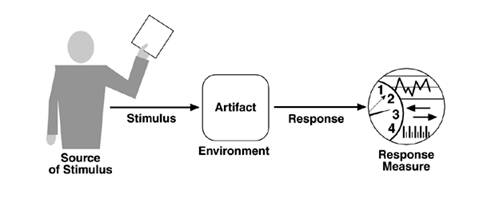
\includegraphics[scale=0.8]{QualityAttributeScenario.jpg}

\caption{The parts of a quality attribute scenario}
\label{fig:Quality_Attribute_Scenario}
\end{figure}





\noindent
One of the core aspects of the definition of software architecture, is that software architecture is a set of structures, which we can use to reason about the system. To assist and visualize these structures, elements, relations and properties we use Module-, Component \& Connector (C\&C)- and Allocation viewpoints \cite{3+1}. 

\begin{enumerate}
    \item Module viewpoint is concerned with how functionality of the system maps to static development units. The focus will be on elements such as classes and interfaces and relationships such as associations, generalizations, realizations and dependencies.
    \item Component \& Connector viewpoint is concerned with the runtime mapping of functionality to components of the architecture. Components are the executing things that perform a function. Connectors are the communication channels between components. The purpose is to focus on the flow of data and responsibilities such as a network call or method call etc.
    \item Allocation viewpoint is concerned with how software entities are mapped to environmental entities. Here the focus are on the physical stuff such as computer or a network. We specify the environment in order to make the software running. 
\end{enumerate}

\noindent
These viewpoint originates from $3+1$ article \cite{3+1}, where the $+1$ is the architectural requirements. These architectural requirements can be formulated through QAS.\\

\noindent
We will discuss different tactics on software architecture for achieving the business goal for the electronic voting application. A tactic according to Bass et al. is defined as.

%**************************************Definition Tactic
\begin{defi}[\textbf{Tactic}]
Tactic is a design decision that influences the achievement of a quality attribute response. \cite{Bass}
\end{defi}
%**************************************Definition Tactic End

\noindent
We will introduce a case which gives an overall description of how a user creates a vote through an electronic voting application. The purpose of the case is describing business/mission requirement of the electronic voting application. Here we will emphasize that it should be clear it reflects the security requirements from the first part. We use the general security requirement for an electronic voting scheme described in chapter 2 as functional requirements for the application. These requirements are well studied and discussed and should be comprehensive for an electronic voting scheme.
    
    \section{Method}
To ensure a solid systematic approach for this part of the thesis we will use   


\begin{enumerate}
    \item Case
    \item Functional requirements
    \item Quality attribute workshop
        \begin{enumerate}
            \item Quality attributes
            \item Quality attribute scenario
        \end{enumerate}
    \item Architectural decision
       \begin{enumerate}
            \item Tactics and patterns
        \end{enumerate}
    \item Architectural evaluation
\end{enumerate}


\begin{description}
    \item[Case] The purpose of the case is an informal description of the requirements for the electronic voting application. We use this as a introduction to a business/mission for the most important requirements for the electronic voting application.
    
    
    \item[Functional requirements]  The purpose of the functional requirement is to capture the electronic voting application behavior based on the case description. We will take these requirements an categorize them according to the security requirements. Event though the functional requirements isn't in focus in this thesis we will use these requirements helpfull information in the discussion part of the Quality attribute workshop.  
    
    \item[Quality attribute workshop]  The purpose of the Quality Attribute Workshops (QAWs) is a systematic method for identifying a system's architecture critical quality attributes, such as availability, security and modifiability, that are derived from mission or business goals. For the scope of this thesis we will follow the phases in the QAW on a theoretical level, to derive the most important QA for the electronic voting application. We will use the structure of the QAS but we will not hold a practical workshop.  Based on the QA we will formulate the most important Quality attribute scenarios and describe related tactics.
    
    \item[Architectural decision]  This part is about describing the rationale behind the architectural decision. Questions such as what made us end up with this design should be clear. A decision also exclude another decision which should also be reflected in this part. We will use Tyree and Akerman approach for describing our decisions. 
    
    \item[Architectural evaluation]  Evaluating a software architecture is about whether the system meets the quality requirements. Here we will cover how well our architecture meets the quality goals in relation to tradeoffs between quality attributes. We use ATAM analysis for this purpose.  

\end{description}
    
    \section{Case}
A user applies for voting for a given election and a registration authority will either accept or reject his application.  If the user is accepted then he should be able to logon a voting page and cast his vote.  When all the registered voters have casted their votes or a deadline is reached, the system should tally the votes and then publish the result on a webpage. Offcause only valid votes are included in the talliering process. The tally process should be handled by registered talliers. During this process none of the talliers should be able relate a  vote to a voter. Nor should a tallier be able to manipulate the talliering process by either adding, removing or alter votes. Each tallier should be hold accountable for his participant in the talliering process. If the tallier is discovered in cheating he is replaced by another tallier during the tallier process. This replacement should not have influence on the result nor should it required re-election. 
    
    \section{Functional requirements}
The description of the requirements of a general voting application can be found in the security requirement section. In this section we will discuss these requirement and how they fit into our electronic voting application.





\begin{description}
    \item [Voter Privacy]
        No one should be able to link a vote back to the specific voter, and only the voter should
        know his vote. These requirements shall hold during and after the election.  
    
    \item [Eligibility]    
        Only Eligible and registered voters can vote. 
    
    \item [Uniqueness]
        Only one vote per registered voter should be counted.
    
    \item [Fairness]
        None should be able to gain any knowledge of the outcome of the election, before the ending. This is to prevent voters of voting accordingly to any leaked information. 
    
    \item [Uncoercibility]
        Nobody should be able to extract the value of a vote. This is to prevent anybody from compelling a voter by force, intimidation, or authority to cast a vote in a specific way. 
    
    \item [Receipt-freeness] 
        The voting system should not produce a receipt that reveals any information about the casted vote. This is to prevent a vote from trading his vote. 
    
    \item [Accuracy] 
        The final tally should be correctly computed from valid casted votes. It should not be
        possible to manipulate the final tally without being detected. 
    
    \item [Universal Verifiabilit]
        It should be possible for any participants and observers to validate individual votes as well as the final tally of the election. 
    
    \item [Individual Verifiability]    
        Every registered voter should be able to verify that his vote is counted correctly. 
    
\end{description}

    
    \section{Architectural requirements}    
\subsection{Quality Attributes workshop}

\subsubsection{2. Business / mission presentation}

På baggrund af den brede formulering af TM16 har vi valgt at udforme en mission præsentation af TM16, med vores vision for TM16. Mission Presentation danner grundlag for QA workshoppen og med en for bred specifikation af TM16 vil vores scenarie kunne misforstås. 


Vi har valgt at anse TM16 som et redskab i et screen forløb af en patient. Når en patient indgår i et screen forløb stilles en måler med TM16 til rådighed. Patienten skal så over en given periode løbende fortage målinger. Når perioden er gået, har fagpersonale mulighed for at inddrage målingerne i evalueringen af patienten over den givne periode. 


Det skal være muligt at benytte TM16 uden internet adgang, da vi ikke kan antage at alle patienter har internet adgang i hjemmet. I tilfælde af at der ikke har været internet adgang under en måling, så sendes denne måling til en intern database på måleenheden. Måliningen sendes til TM16 Server så snart etableres en internet forbindelse.



TM16 skal væres nem at betjene da patienterne har meget forskellige faglige baggrund, hvor vi må antage at nogle af patienterne har meget ringe eller ingen teknisk færdigheder. 

Det skal desuden være muligt for fagpersonalet at arbejde med målingerne fra TM16 i deres eget fagprogram dvs. et specifik program til specifikke faggrupper. Det forventes at målingerne kan trækkes direkte fra TM16 så snart at målingerne at sendt til TM16 server. Da TM16 forventes at blive en kæmpe succes så vil der komme stor tilgang af brugere og sandsynligheden for samtidighed vil dermed opstå. Derfor skal systemet kunne håndter samtighed. Vi formoder at i takt med at flere faggrupper får adgang til TM16, så vil der blive stilet krav til flere forskellige typer målingerne.

\subsubsection{4. Identify architural drivers}
Voter point of view: \\
Usability: Easy to use for a voter\\
Usability: Trustworthy should give detailed feedback\\
Availability: available when needed\\\\


\noindent
Owner point of view:\\

\noindent
Robustness:\\
Scalable: Should be able to handle a large amount of user within a reasonable time\\
Testability: Given the nature of systems complexity it should be easily testable to ensure robustness and reliability\\
Security: The integrity should withhold even though if cheating occurs.\\

\noindent
Universal verifiability\\
Interoperability:Not only participant but also passive observers should be able to validate through out the election and afterwards(Fairness)\\


\noindent
Future proof\\
Modifiable: only a registered user should be able to vote. This registration should be easily replaceable depending on the nature of the election.\\
Modifiable: The system should modifiable such that core elements are replaceable\\








\subsubsection{5. Scenario brainstorming}

\subsubsection{6. Scenario considation}

\subsubsection{7. Scenario prioritization}

\subsubsection{8. Scenario Refinement}
        
        
    
    
\clearpage
%***************************************************************
%               Part 7: Implementation in practices
%***************************************************************
\chapter{The application}
    In chapter \ref{chap:application} we described the theoretical aspect behind our system. A software architecture was designed and the most significant scenarios was formalized and solved on a theoretical level. In this chapter we describe how we implemented the design into a application.    

%********************************************************************
\section{Introduction}
%********************************************************************
Implementing a software design can be a difficult task, as design modules rarely maps directly into code. Using the approach of different viewpoints and scenarios helps in this regard, but challenges due arise which could not have been foresee nor illustrate in the design phase. Challenges can come from our design of the development environment to the physical restricts of the deployment environment. 

%********************************************************************
\section{Method}
%********************************************************************
The final result is described in a top-down approach, We start with an informal description of the system, and from here gradually go into details starting with the module views which describes the static structures of the implementation. Then, follows the component and connector view to describe the dynamic structures. After the presentation of the implementation we will look at how the specific tactic have been implemented and how we have taken solved the functional requirements of an electronic election.

%********************************************************************
\section{Development environment}
%********************************************************************
The implementation have been done using Microsoft ASP.NET framework, C\# and Javascript programming language. ASP.net is a widely used and supported framework for creating web application. This framework is used both as the backend RESTful server, BulletinBoard and for the web server hosting the clients. The clients, voter and tallier is implemented using javascript. Javascript have the benefits of running inside all modern browser and is widely used, thous giving us a very large set of libraries to our disposal. \\


\section{Final result}
In this section we describe the final implementation of the software design. 

%********************************************************************
\subsection{Overview}
%********************************************************************

\begin{figure}[H]
    \centering
    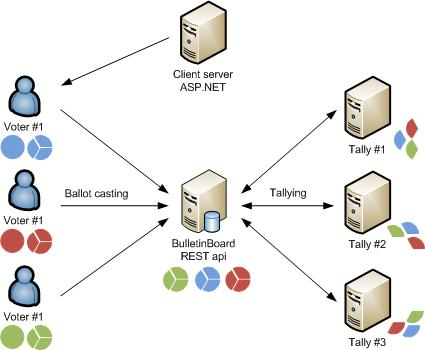
\includegraphics[scale=0.90]{Overview.jpg}
    \caption{Overview of the system}
    \label{fig:informal_overview}
\end{figure}

The figure \ref{fig:informal_overview} above illustrates an overview of system and the information flow in the different phases of the protocol. From left to right we see the voters each casting there votes and hiding the votes within a secret which, though secret sharing, is divided and encrypted into pieces corresponding to the number of talliers. the ballot casting phase ends with the voters publishing there votes and secret to the BulletinBoard. Ending the Ballot casting phase starts the tallying phase where the talliers each collects there individual pieces of the secret, multiplying the shares together, decrypting the multiplum and publishes the decrypted multiplum to the BulletinBoard. The last segment of the tally phase, where the votes are calculated is not illustrated in the figure, but is none the less implemented by letting a dedicated tally do the calculating and posting the result to the BulletinBoard. \\

\noindent
The overview does not introduce many new elements to the implementation not previously known from the protocol, in fact the only new element introduced is the Client server which serves as a web-server for the voters, to which the voters logon in order to cast there votes. However the overview clearly shows the topology of the implementation, namely a star topology with a server (BulletinBoard) in the middle and Clients all around. There is no directly communication between the clients, all communication goes through the Server. This is due to the nature of an election, though we require the talliers to have a persistent connection to the server we don't expect voters to stay connected throughout an entire election. The reason the Bulletinboard needs to have an persistent connection to the talliers is because after the ballot casting phase, The Bulletinboard needs to be able to notify the talliers for tallying phase.

%********************************************************************
\subsection{Viewpoints}
%********************************************************************
We use viewpoint as we further describes the implementation in details. We start with the module view points which shows the static elements of the implementations, elements like packages, interfaces and classes.  \\

%********************************************************************
\subsubsection{Module view}
%********************************************************************
Starting from the top we look at how the implementation is structured into packages, where each packages contains elements that focuses on the same responsibility. Structuring our implementation this way follows the design principles of high Cohesion and low Coupling introduced in chapter \ref{chap:application} and lays the ground for code that is flexible and easily maintainable. 

\begin{figure}[H]
    \centering
    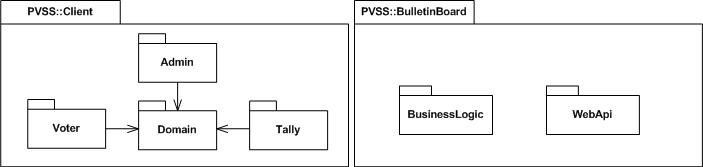
\includegraphics[scale=0.60]{Moduleview_packages_overview.jpg}
    \caption{Package overview}
    \label{fig:package_overview}
\end{figure}

\noindent
Figure \ref{fig:package_overview} shows a package overview of the entire implementation. The figure show both the packages included in the implementation of the Client and the Bulletinboard. The Client include packages containing logic specific for Voter, Tally, Admin and the Domain package which holds logic used across the Client. The package overview of the Bulletinboard with only the two packages BusinessLogic and WebApi looks on the surface very simply, but below we unfold each package showing a more complex structure. 

\begin{figure}[H]
    \centering
    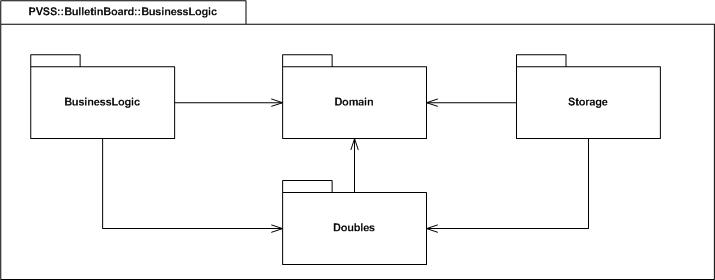
\includegraphics[scale=0.60]{Moduleview_packages_BulletinBoard.jpg}
    \caption{Package overview of Bulletinboard business logic}
    \label{fig:package_overview_of_bulletinboard_businesslogic}
\end{figure}

\noindent
Figure \ref{fig:package_overview_of_bulletinboard_businesslogic} shows the packages revealed when unfolding the BusinessLogic package. This include the sub-packages BusinessLogic, Storage, Doubles and Domain. The packages BusinessLogic, Storage and Domain is fairly self explanatory, the package Double holds the logic we used in order to unit test our implementation. \\


\begin{figure}[H]
    \centering
    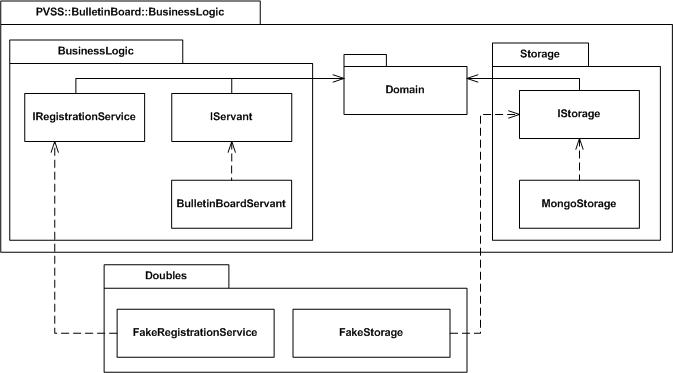
\includegraphics[scale=0.60]{Moduleview_Class.jpg}
    \caption{Module view of Bulletinboard}
    \label{fig:module_over_of_bulletinboar}
\end{figure}

\noindent
Figure \ref{fig:module_over_of_bulletinboar} shows the interfaces and classes within the BusinessLogic package of the Bulletinboard. Note that the package Doubles have been left outside the container of the BusinessLogic, this is due to the fact that its responsibilities only evolves around testing and the packages is not used in the production environment. Also noticeable is the Domain package have not been specified further, the reason for this is, that it simply holds the representation of physical elements like a Ballot, a voter, a share etc, there is no business logic within these classes.

\begin{description}
    \item[IRegistrationService] is an interface that holds the responsibility of the \textit{Registration authority} specified in section \ref{sec:the_voting_process}. Is validates and registries eligible voters.  For this implementation we only included the class \textbf{FakeRegistrationService} which implements responsibilities from the IRegistrationService. 
    
    \item[IServant] is an interface that have the responsibilities of the \textit{BulletinBoard} also the described in section \ref{sec:the_voting_process}. It handles the communication with the Clients and insures the persistence of the election data such as the ballots, the shares etc. The class \textbf{BulletinBoardServant} implements the responsibilities of the IServant. A key functionality of the BulletinBoardServant is that most of its methods is read-only, this helps to ensure that no honest or dishonest user removes information. 
    
    \item[IStorage] is an interface that have the responsibilities of persisting and retrieving data. Both the classes \textbf{MongoStorage} and \textbf{FakeStorage} implements the responsibilities of the IStorage. The \textbf{MongoStorage} also acts as a client to a Mongo database to which it stores the data, where the \textbf{FakeStorage} simply stores the data in memory, meaning that the data is lost when the application stops. 
    
\end{description}

\begin{figure}[H]
    \centering
    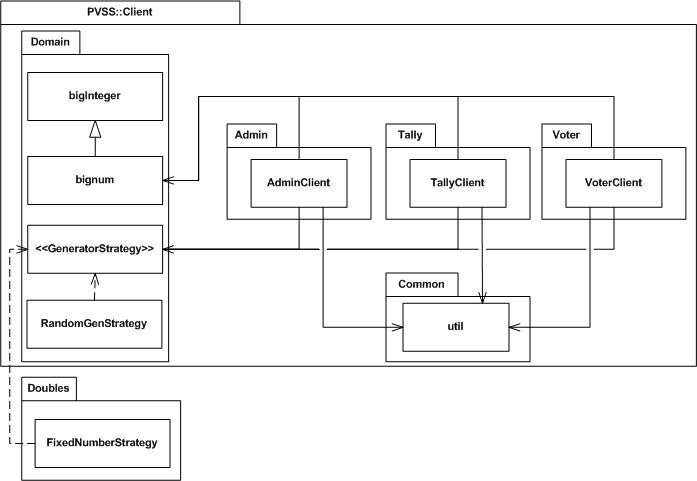
\includegraphics[scale=0.60]{Moduleview_Class_Client.jpg}
    \caption{Module view of Client}
    \label{fig:module_view_of_client}
\end{figure}

\noindent
Figure \ref{fig:module_view_of_client} shows the interfaces and classes of the Client. Again the package Double is left outside the contain of the Client, due to the same arguments stated above. 

\begin{description}
    \item[util] is a simple class that holds some helper function, that is used a cross he system. 
    
    \item[bignum] is a class that inherits the functionlitites from its superclass \textbf{bigInteger}. This structure enables us to expand or alter the functionalities of the \textbf{bigInteger} without changing the class. 
    
    \item[INumberGenerator] is an interface which have the responsibility of generating random integers and primes. The classes \textbf{RandomGenStrategy} and \textbf{FixedNumberStrategy} both implements the responsibilities of INumberGenerator. \textbf{FixedNumberGenerator} is used for testing and enabling us to control the numbers return. 

    \item[AdminClient] is a class that holds the responsibilities of creating an election and generating the public elements used in the election. The AdminClient is depending on the class Bignum, and the Interface INumberGenerator. 
    
    \item[VoterClient] is a class that holds the responsibilities of a \textit{Voter} described in the protocol, section ~\ref{sec:ballot_casting}. This class, like the AdminClient is depending on Bignum and INumberGenerator.    
    
    \item[TallyClient] is a class that holds the responsibilities of a \textit{Tally} described in the protocol, section ~\ref{sec:tallying}. This class, is also depending on the Bignum and INumberGenerator. 
\end{description}

\noindent
This last module view concludes the overall static structure of the implementation, we however have not further specified the elements in the Webapi package shown in figure \ref{fig:package_overview}. The reason for this, is that it does not hold any elements related to the protocol but only elements regarding the implementation of the REST interface describe in the Interoperability tactic in section \ref{sec:interoperability:restapi} and this implementation is discussed later. \\

%********************************************************************
\subsubsection{Component and Connector view}
%********************************************************************
For this next part we will look at how the dynamic components in the implementation interacts during runtime. We will present an overall insight of the system's interaction. 

\begin{figure}[H]
    \centering
    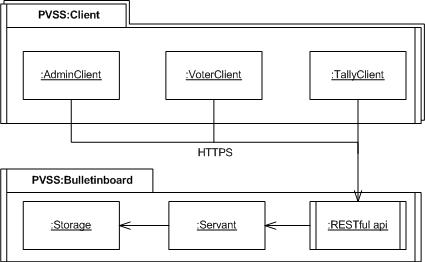
\includegraphics[scale=.7]{CC_Overall_View.jpg}
    \caption{Overall Component and Connector view}
    \label{fig:CC_overall_View}
\end{figure}

\noindent
Figure \ref{fig:CC_overall_View} shows how the system interact overall. As we have seen in the module views, there is no interacting between the components in the Client. They each operates independently and they all communicates with the Bulletinboard through the REST API.  The communication between the Clients and the Bulletinboard is done through an HTTPS connection. This connection uses Secure Socket Layer (SSL) or Transport Layer Security (TLS) to encrypt the messages sent or received. All successful communication done with the REST API is forward to the Servant component that handles the business logic. If there is a need for persisting data, then the Servant sends the data to the Storage. \\

\noindent
The following sequence diagram shows the overall flow of the system from the ballot casting phase to the result. The internal method calls and calculations done on each individual class is not show, in order to present a better overview.  

\begin{figure}[H]
    \centering
    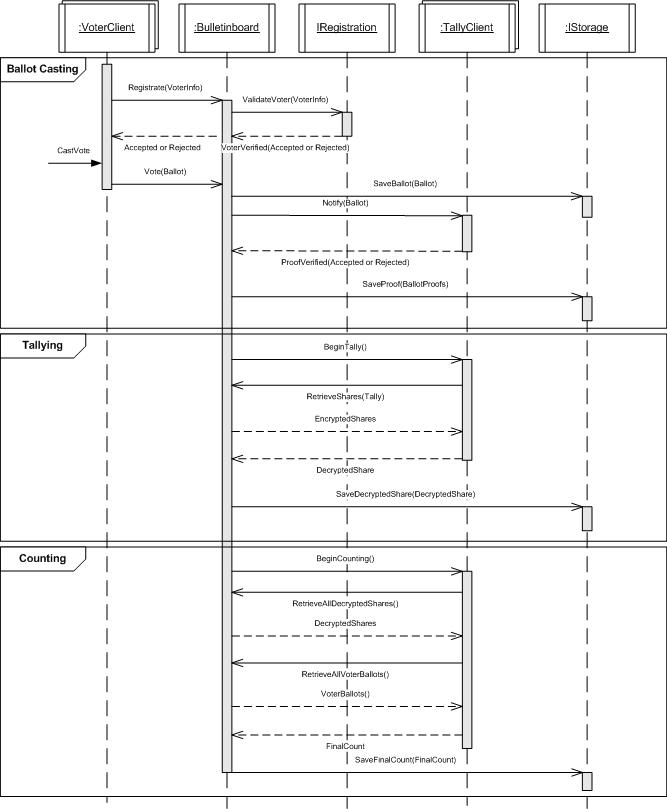
\includegraphics[scale=.7]{CC_SekvensDiagram.jpg}
    \caption{Overall Sequence diagram}
    \label{fig:CC_sequence_diagram}   
\end{figure}

%********************************************************************
\subsubsection{Allocation view}
%********************************************************************
Finishing out the viewpoints we lastly have a deployment view showing the systems requirements to the deployment environment. 

\begin{figure}[H]
    \centering
    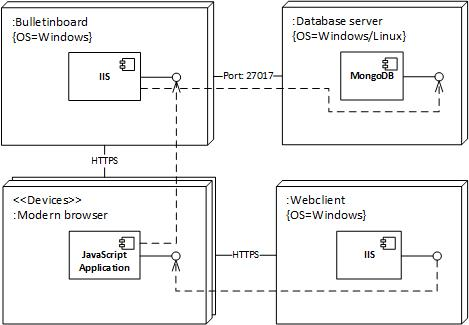
\includegraphics[scale=.7]{deployment_view.jpg}
    \caption{Final deployment view}
    \label{fig:final_deployment_view}
\end{figure}

\noindent
Figure \ref{fig:final_deployment_view} shows that the system requires three servers, a database server running a mongo database, a web-server with a Internet Information Server (IIS) installed to host the Bulletinboard RESTful Webapi and lastly a web-server also with IIS installed to host the Webclient. We also require that devices that is to communicate with the system needs to have a modern browser installed, that is able to execute JavaScripts. 


%********************************************************************
\section{Implementing the tactics}
%********************************************************************
In this section we will highlight selected implementation of previously described tactics from chapter \ref{chap:application}.

%********************************************************************
\subsection{Interoperability: REST API}
%********************************************************************
As stated earlier we use a REST interface which should be easily accessible by everyone. This means that our Bulletinboard is build on some of the REST principles. Figure \ref{fig:rest_electronic_voting_web_service_model} illustrate an informal webservice model which describes our resources on the Bulletinboard. The process of constructing this diagram gives overview and insight of how we could design a REST interface on the different resources. 

\begin{figure}[H]
    \centering
     \makebox[\textwidth]{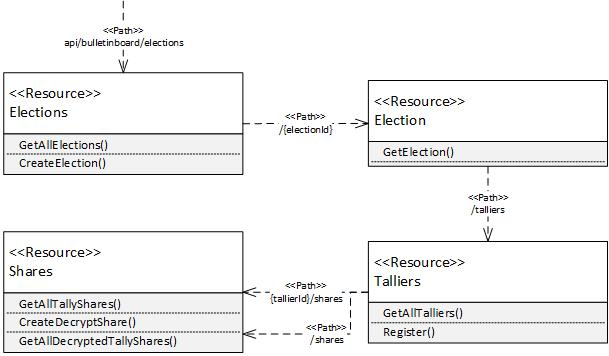
\includegraphics[scale=0.60]{rest-classdiagram.jpg}}
     \caption{Overview of REST electronic voting web service model}
     \label{fig:rest_electronic_voting_web_service_model}
\end{figure}


\noindent
Figure \ref{fig:rest_api_to_the_Bulletinboard} shows our final REST api. The urls shows how the REST api can be accessed together with the HTTP methods which shows which methods can be invoked on the different urls. 


\begin{table}[H]\fontsize{8}{9}\selectfont
\centering
\begin{tabular}{|l|l|l|}
\hline
Resource                                                    & URL                                                & HTTP methods                                                            \\ \hline
Elections                                                   & /elections                                         & \begin{tabular}[c]{@{}l@{}}GET GetAllElections\\ POST CreateElection\end{tabular} \\ \hline
Election                                                    & /elections/\{electionId\}                                  & GET GetElection                                                                   \\ \hline
Votes                                                       & /elections/\{id\}/votes                            & \begin{tabular}[c]{@{}l@{}}GET GetAllVotes\\ POST CreateVote\end{tabular}         \\ \hline
Talliers                                                    & /elections/\{id\}/talliers                         & \begin{tabular}[c]{@{}l@{}}GET GetAllTalliers\\ POST Register\end{tabular}        \\ \hline
Shares                                                      & /elections/\{id\}/talliers/\{id\}/shares           & \begin{tabular}[c]{@{}l@{}}GET GetAllTallyShares \\  POST CreateDecryptShare     \end{tabular}                                                            \\ \hline
\begin{tabular}[c]{@{}l@{}}Decrypted \\ shares\end{tabular} & /elections/\{id\}/talliers/shares        & \begin{tabular}[c]{@{}l@{}}GET GetAllDecrypted\\ TallyShares\end{tabular}                                                        \\ \hline
\end{tabular}
\caption{REST api to the Bulletinboard}
\label{fig:rest_api_to_the_Bulletinboard}
\end{table}


\noindent
Since our webclients is build purely on javascript, all communication is through ajax call to the Bulletinboard. Listings \ref{lst:javascript_rest_api} illustrates how one can interact with REST api. The example shows how to create an election. This is called by the Admin client which starts the election.   \\ 


\begin{lstlisting}[language=Javascript, caption=Javascript example, label=lst:javascript_rest_api]
    $.ajax({
        type: "POST",
        url: "api/bulletinboard/elections",
        data: jsonData,
        success: function (data) {
            if (callBack)
                callBack(data);
        },
        contentType: "application/json"
    });
\end{lstlisting}


 
%********************************************************************
\subsection{Modifiability: Number generator}
%******************************************************************** 
Implementing this tactic proved to be fairly easy. However as the dynamic nature of Javascript does not support the concept
of interfaces as we know it from Java and C\#, we had to introduce a method to secure that the injected NumberGenerator strategy
applies to its responsibilities. To construct this method we utilizes the concept of \textit{Duck Typing} which basically states that
if an object walks like a duck and quarks like a duck, then to the concerns of Javascript it is a duck!. 

\begin{lstlisting}[language=Javascript, caption=Implementation of Duck typing, label=lst:ducktyping]
    // example duck typing method
    var InterfaceMethods = function (obj /*, method list as strings */) {
        var i = 1, methodName;
        while ((methodName = arguments[i++])) {
            if (typeof obj[methodName] != 'function') {
                return false;
            }
        }
        return true;
    }
\end{lstlisting}

\noindent
In the following listing \ref{lst:interface_randgen} we show how the InterfaceMethod method is used to check
for an interface object. It checks if the methods specified in the parameters is to be found on the object passed as the 
first parameter. In the example below it checks for the methods "randBetween" and "randPrimeBetween".

\begin{lstlisting}[language=Javascript, caption=Checking for an interface, label=lst:interface_randgen]
var voterClient = function (serv, options) {
    ...
    ...
    var randomGen;                     

    if (options) {
        if (options.randomGen) {
            if (util.InterfaceMethods(options.randomGen, 'randBetween', 'randPrimeBetween')) {
                randomGen = options.randomGen;
            }
        }
    } 
\end{lstlisting}
 
\noindent
As shown in the listing \ref{lst:interface_randgen} the NumberGenerator strategy is simply injected
into the VoterClient upon creation. Methods within the VoterClient can now execute the methods
randBetween and randPrimeBetween on the injected object through the variable randomGen. 
 
 

%********************************************************************
\section{Challenges}
%********************************************************************

%********************************************************************
\subsection{Parsing a custom class}
%********************************************************************


%********************************************************************
\subsection{Same-origin security policy}
%********************************************************************
Access-Control-Allow-Origin
- CORS

%********************************************************************
\subsection{Generating Prime}
%********************************************************************
Generating very large primes is a computationally hard task and thous time consuming. Given the fact
that the prime $q$ used in our implementation is public known, it is easy to think that one could simply
use one or a set of very large hardcoded primes. However, by performing a large precomputation for a given
prime an adversary can quickly calculate arbitrary discrete logarithms in that group, efficiently reducing 
computation cost for all targets that uses this group \cite{Adrian:2015:IFS:2810103.2813707}. 

%********************************************************************
\section{Analyzing the application}
%********************************************************************
We will in this section analyze of implementation. We will analyze the chosen tactics, the code quality and evaluate the security in the implementation. 

%********************************************************************
\subsection{Electronic voting secure requirements}
%********************************************************************
\begin{description}
    \item[Voter Privacy]
        No one should be able to link a vote back to the specific voter, and only the voter should
        know his vote. These requirements shall hold during and after the election.  
        
        This requirement is meet by our implementation, infact its one of the core elements in the
        Election voting protocol from section \ref{sec:the_protocol}. Every voter only publish his vote
        though $U = G^{v+s}$ where $G$ is a generator and $v \in \{0,1\}$ and $s \in \Z_q$. As $s$ is only
        known by the voter and is uniformly random picked then the sum of $s$ and $v$ is also unknown for any 
        potential adversary under the security of the DL problem. And one could ague that even if an
        adversary should be break the DL problem then, unless he knows $s$, the vote $v$ would still
        be unknown. 
        
        
    \item[Eligibility]
        Unlike Voter Privacy, this requirement of non-eligible voters not being able to vote is not
        fulfill by the protocol it self. We handle this in our implementation though the registration service
        describe in section \textcolor{red}{[???]}. This enable us to change the registration service 
        accordingly to the nature of the election.         
        
        
    \item[Uniqueness]
        Uniqueness is about making sure only one vote is counted for each eligible
        voter. 
        
    \item[Fairness]
        To ensure all participants get a fair election, no partial tally must be
        revealed before the end of the voting. This is achieved in our implementation
        by only starting the tally phase when all votes are casted or when a deadline is 
        reached and the ballot casting phase ends. The Talliers in notified only by the Bulletinboard
        when to start the tally phase thou none other have the authority to do so.  
        
        Through the property of secret sharing used in the protocol, the secret to decrypt the
        vote is shared amoungst three or more talliers. These shares are again encrypted with the public key 
        of the corresponding tally. As a consequence, no one except the tally with the corresponding
        private key is able to decrypt the share.
        
        
         
    \item[Uncoercibility]
        Participating voters are able to vote freely, without anyone able to coerce
        them into casting a vote in a particular way. In addition, no authority should be able to extract the value of a vote.
        
    \item[Receipt-freeness]
         The voting system should not produce a receipt that reveals any information about the casted vote. This is to prevent a vote from trading his vote. 
         Our implementation only confirms the success of a voting, not the value of the vote. There is no functionality that enables any participants nor observers to
         gain information about the value of a vote. 
         
        
    \item[Accuracy]
        The final tally should be correctly computed from valid casted votes. It should not be
        possible to manipulate the final tally without being detected. \\
        
        \noindent
        Our implementation utilizes the proofs from the protocol to fulfill this requirement. 
        
        \noindent
        Under the Ballot casting phase of the protocol, we require that the voters proofs the correctness of there votes. This is done though the $Proof_U$ and $DLEQ$ proofs, which is required to be published along side the encrypted vote $U$. Should one of the proofs fail, then the vote is marked invalid and this vote is ignore in the preceding processes. 
        
        \noindent
        In the tally phase of the protocol, the tally multiplies its shares and then decrypts them and publishes the end result. Along with this result we require that the $DLEQ$ proof is published aswell. This allows us to verify the correctness of the tallying process for each tallier. Should a $DLEQ$ proof from a tallier fail then the tally's shares is ignore in the preceding process. The protocol requires the shares from at least $t$ talliers, in order to extract and calculate the end result. Should it 
        be the case that this requirement is not fulfill an re-election is require but untill then the implementation simply ignores the shares from the tally in question.
        
        \noindent
        Should an adversary gain access to the database serving the BulletinBoard, it would be possible for this adversary to manipulate the verdict of a proof but not
        the proofs them self, as the construction of the proofs prevent this. Thou our implementation does not take this scenario into account it would be fairly easy to make
        a functionality that reevaluates the proofs should such a breach have been detected. One could argue that an adversary with full access to the database could also remove elements such as a casted vote or the information that a given voter have voted. The later would effectually enable the given voter the ability to double vote, this scenario is not handled in our implementation. The first scenario is also possible but given the fact that our implementation have voter privacy and the votes is secure under the DL problem then the adversary would not know if he is removing and "no" or a "yes" vote. 
        
        
    \item[Universal Verifiability]
        It should be possible for any participants and observers to validate individual votes as well as the final tally of the election. 
        
        \noindent
        The protocol is basically designed around this requirement and as such most of the information is published to the Bulletinboard, and as describe under the requirement "Accuracy" our implementation requires both the voters and the talliers to publish proof of the correctness and the consistency of the vote and the shares to the BulletinBoard. 
        
        \noindent
        Everything on the BulletinBoard is publicly available both for participants and none participants of the election. $Proof_U$ verifies that an encrypted vote $U$ is either 0 or 1 and the DLEQ proofs verifies the consistence of the shares for both the voters and the talliers. The end result can be calculated from the publicly known information available after the tallying phase. 
            
    \item[Individual Verifiability]
        Every registered voter should be able to verify that his vote is counted correctly. 
        
        \noindent
        in our implementation there is no link between a vote and a voter when the  
        
        It would be desirable if a voter could be able to check that his encrypted vote
        was counted and tabulated correctly in the final tally. The problem is that
        the combination of receipt-freeness and individual verifiability requirements
        obviously conflict with each other. One would need some kind of receipt in
        order to achieve verifiability, but then the same receipt could be used for
        vote buying or selling. As a consequence this voting application has given
        preference to receipt-freeness and thus no functionality for verifying votes
        later in the process are implemented.
        

\end{description}

%********************************************************************
\subsection{Security analyze}
%********************************************************************
In Section \ref{sec:security_requirements} several security requirements that a secure 
and complete cryptography voting protocol should satisfy where listed. We will look at
these requirements and see if our implementation satisfy these. We will also 

%********************************************************************
\section{Lessons learned}
%********************************************************************


\part{Reflecting}    
\clearpage    
%***************************************************************
%               Part 8: Discussion
%***************************************************************
\chapter{Discussion}
In this chapter we will discuss and reflect our challenges regards to our work with this thesis objectives. 



%********************************************************************
\section{Theoretically}
%********************************************************************
The learning curve has been steep regards to learning the electronic voting protocol. The literature is on a very high mathematical academic level seen from the perspective of a software developer. We see this is as a challenge that a protocol is only described for such a narrow audience, especially  one that requires knowledge of such a specific field as cryptography. Most of the concepts used to describe the protocol assumes a certain background knowledge. When reading the article on protocol there is often reference to other literature that the protocol is build upon. This makes the article hard to read, as the reading flow is interrupted. \\

\noindent
With this thesis we have tried to break down the protocol such that it is understandable for a broader audience. We have constructed this thesis such that the reader gradually gains the required mathematical knowledge to understand the basic elements of the protocol. The description of the protocol has been divided into a basic and a detailed description. The basic description will give the reader basic knowledge about the protocol and should provide enough knowledge for a simple implementation of the protocol. Of cause this simple implementation will not fulfill all the security requirements for an electronic voting application.


\subsection{Knowledge accumulation}
Starting this thesis we had the subjects of multiparty computation and secure secret sharing in mind, but after guidance with our supervisor we agreed on working with the electronic voting protocol described in \cite{Schoenmakers1999}. In order to connect the theoretically part of the thesis with the practical part, we felt that additionally knowledge about electronic voting in generally were needed. After reading other articles on the subject we got a better overview on the concepts of electronic voting. It turns out that the security requirements for electronic voting is one of the key elements linking the theoretical part together with the practical part. This research helped us being able to include different issues, that we by our self would not consider immediately, such as our consideration regarding \textit{Eligibility} and our reflection on the \textit{Individual verifiability}. In general our research on the subject have given us a more critical approach to which security parameter we will have to take into consideration. For example we have given a short description of different known attacks on the discrete logarithm problem. Knowing these different attacks gives knowledge for how large $q$ must be, which is essential for our practical part.   


%********************************************************************
\section{Practical}
%********************************************************************
We have spend much time on understanding the protocol and the security requirements regarding electronic voting. This has been costly for the practical part of this thesis. We have not been able to develop a complete application, but rather a proof of concept, where we have tested the protocol and our architectural strategies. We would like to have spend more time on the practical part so that we could have tested our QAS such as performance and the availability. Since these two attribute is central for a software architecture on a large scaled application. \\

\noindent
Basically the entire protocol is about doing computations such as exponentiation, multiplying, addition,  modulo reduction, hash functions and generating random large primes etc. Doing it and doing it right is a challenge - all these computation together  makes the system complex and challenging to debug. We created several proof of concept with small numbers, which was manageable to follow. We haven't found a optimal way yet for debugging the computations with large numbers. \\

\noindent
As developers we are concerned with achieving maintainability and readability of the code, therefor code quality is an important aspect to take into account. The protocol works with variables like $g$, $G$, $Y$, $Y^*$, $DLEQ$, and $Proof_u$ etc. We ask our self what is the best naming conventions for these variables. Our naming conventions is based on trying to be consistent and give variables signing names.  


%********************************************************************
\subsection{Generating Prime}
%********************************************************************
Generating very large primes is a computationally hard task and thus time consuming. Given the fact
that the prime $q$ used in our implementation is public known, it is easy to think that one could simply
use one or a set of very large hardcoded primes. However, by performing a large precomputation for a given
prime, an adversary can quickly calculate arbitrary discrete logarithms in that group. And efficiently reducing the computation cost for all targets that uses this group \cite{Adrian:2015:IFS:2810103.2813707}. 


%********************************************************************
\subsection{Individual Verifiability} \label{sec:discussion_individual_verifiability}
%********************************************************************
Here we will elaborate on these two informal requirements from section \ref{sec:analyzing_electronic_voting_secure_requirements} regarding \textit{Individual Verifiability}. 

\begin{enumerate}
    \item All votes from the ballot casting is included in the final tally.
    \item Every votes from the ballot casting is calculated correctly.
\end{enumerate}

\noindent
As stated earlier our job is to convince the voter about the above statements. If this is possible, we mean that we have argumented for our statements and thereby the security requirement. To elaborate these requirements we will need some illustration of the ballots and the tallying phase. Figure \ref{fig:discussion:ballot_casting_and_tallying_phase} shows a simplified list of all valid ballots from the ballot casting phase. Figure \ref{fig:discussion:ballot_casting_and_tallying_phase} also shows a simplified list of the multiplied shares and the corresponding proofs by each tally.\\

\noindent
As for the first statement we refer that anyone can verify the correctness of the votes and the consistency of each share. By definition all is public and anyone are able to verify the validity of the outcome of the proofs under the election.\\

\noindent
So if the list is trusted and accepted by everyone then with high probability we can say it is correct. To ensure that all ballots are included in the final tally we have to be convinced, that each of the shares are included in the tallying phase. Each tally will compute $Y^*$, $S^*$ and a proof based on the shares belonging to them. The key is that anyone are able to confirm the $Y^*$ to ensure that all shares are included in the computation of $Y^*$. As for the second statement all can verify that the decryption of the shares are done correctly. All information needed in order for calculating the final tally is publicly available on the bulletin board and thus anyone are able to recalculate the final tally.      

\begin{figure}[H]
    \centering
    \captionsetup[subfigure]{labelformat=empty}
    \begin{subfigure}[b]{0.45\textwidth}
        \begin{table}[H]
            \centering
            \begin{tabular}{|l|l|}
                \hline
                \multicolumn{2}{|l|}{Ballot casting} \\ \hline
                Ballot   & Valid              \\ \hline
                1        & Yes                \\ \hline
                2        & Yes                \\ \hline
                3        & Yes                \\ \hline
                4        & Yes                \\ \hline
                5        & Yes                \\ \hline
                6        & Yes                \\ \hline
            \end{tabular}
        \end{table}
        \caption{Ballots with proofs validation}
    \end{subfigure}
    \qquad % <----------------- SPACE BETWEEN PICTURES
    \qquad % <----------------- SPACE BETWEEN PICTURES
    \begin{subfigure}[b]{0.40\textwidth}
        \begin{table}[H]
            \centering
            \begin{tabular}{|l|l|l|l|}
                \hline
                \multicolumn{4}{|l|}{Tallying phase}       \\ \hline
                Tally & $Y^*$ & $S^*$ & Valid                    \\ \hline
                1     & 10 & 3  & Yes                      \\ \hline
                2     & 8  & 9  & Yes                      \\ \hline
                3     & 5  & 8  & Yes                      \\ \hline
                4     & 9  & 4  & Yes                      \\ \hline
                5     & 9  & 3  & Yes                      \\ \hline
                6     & 2  & 8  & Yes                      \\ \hline
            \end{tabular}
        \end{table}
        \caption{Tallying phase}
    \end{subfigure}
    \caption{Tables showing the states of a Ballots and Tally shares after each phase in a election}
    \label{fig:discussion:ballot_casting_and_tallying_phase}
\end{figure}



\section{Lesson learned}
Looking back, we should have been better at narrowing the scope of the theoretical part of this thesis.  However this is a hard task with our  experience within the field of cryptography. With our programming experience and our knowledge in the field of software we can certainly say it has not been a trivial task to implement and at the same time getting the required knowledge of the different parts of the protocol. As a consequence we had to prioritize the project using the elements of "The Project Manager's Three-Legged Stool". Here we have three elements time, cost and quality which are parameters in a project. For this thesis time and cost are relatively fixed, which leads to one parameter to adjust namely quality. As stated earlier there is still work for us to do, on the practical part of our application. \\

\noindent
Our choice of development environment has been Visual Studio with ASP.NET, C\# and Javascript as main programming languages. Based on our knowledge that these technologies is widely used within our profession, the choice was clear for us. We have encountered challenges in our process to gather knowledge about certain technical aspects, revolving different cryptographic libraries in our development environment. The documentation for these libraries covering our development environments have been poor. A consequence of this have been that we have use more time then planned, on our application. We have read a lot of forums and documentation using other technologies on this subject. An recommendation will therefor be that one should be careful when choosing the tools to implement an application in this field. 










\clearpage
%***************************************************************
%               Part 9: Conclusion
%***************************************************************
\chapter{Conclusion}
In this thesis three objectives were studied: The theory behind Shamir secret sharing and multiparty computation as well as the cryptographical concepts needed to understand it. The electronic voting protocol and the mathematical justification behind it. Design and implement an secure and scalable web based electronic voting application based on the protocol. We will in the following summarize our main achievements. \\

\noindent 
By combining the theoretical knowledge gained through session with our supervisor and through studying the field of cryptography, with applied practical experience gained by implementing the protocol in a proof-of-concept application. We have accomplish, most of the objectives in this thesis.

\begin{enumerate}
    \item We have gained comprehensive knowledge in regards to Sharmirs secret sharing and multiparty computation as well as the concepts surrounding them. Furthermore we feel that we have managed, through elaboration and the use of examples, to describe these concepts in such a way that peers with a similar backgrounds as us, as a software developers, can learn the concepts with a lesser steep learning curve. 
    
    \item We have taken the description of the PVSS protocol and the electronic voting protocol described in \cite{Schoenmakers1999} merging them together, for then to divide the description into three different parts each elaborating the protocol further. We see this structure as an optimal way for learning the protocol while trying the concepts in practice, as it allows for iterative implementing the protocol. 
\end{enumerate}    


\noindent  
Gaining knowledge about the theoretical concepts behind the protocol, have helped us understand how to implement the protocol. Even though we have practical programming experience, we none-the-less faced several situations where the theory helped us clarify how to solve the situation.    
    
\begin{enumerate}   
    \item While implementing the electronic voting application we had the chance to combine the theoretical knowledge with our programming experience. This has been a huge advantage in our learning process. One thing is to understand the mathematics behind the protocol. Another thing is knowing what is needed in order to implement the protocol. 
    We have found it beneficial to gain comprehensive knowledge of the mathematics and cryptography concepts behind, not only the protocol but also electronic voting in general. This unfortunately have been more time consuming then expected, which in the end had the consequence that we have not yet reach our objective with our application. Nevertheless  
    we got insight into designing and implementing a cryptographic protocol.
    
    \item Our design of the electronic voting application have been heavily influenced by the security requirements for electronic voting. We see these requirements as an essential part of developing an electronic voting application. While most of the requirements is taken into account by the protocol it self, there where some requirements that we had to incorporate into the application our-self. Even though our web based electronic voting application is not finished, we have prepared an architecture which is build upon known design principles from \cite{Bass} and \cite{Baerbak10} such as Quality attributes (QA), Quality attribute scenarios, tactics and design patterns. Furthermore we would like to highlight these QA, \textit{Interoperability}, \textit{Modifiability}, \textit{Security} and \textit{Testability} which the architecture is build upon.        
\end{enumerate}
\clearpage
%***************************************************************
%               Bibliography
%***************************************************************
\addcontentsline{toc}{chapter}{\\BIBLIOGRAPHY}
\bibliographystyle{alpha}
\bibliography{901_Bibliography}

\clearpage
%***************************************************************
%               Appendex
%***************************************************************
\appendix
\addcontentsline{toc}{chapter}{\\APPENDICES}
\chapter{Proofs}
%----------------------------------------------------------------------
\section{$DLEQ$ non-interactive proof between voters and verifier}
\label{sec:dleq_non-interactive-proof-between_voters_and_verifier}
%----------------------------------------------------------------------
In section \ref{sec:dleq_voter_verifier} we elaborated an interactive $DLEQ$ proof between voter and verifer. Here we present how one can turn an interactive proof to a non interactive proof. This is also known as the Fiat Shamir where we are transforming an interactive proof into a non interactive proof which is described in section ~\ref{sec:fiat_shamir}. Instead of the verifier computes a challenge, the prover computes the challenge as a random function as described in \ref{sec:hash_function}.  We will present two ways off doing this transformation, a non optimized and an optimized version. Last we will describe an example on how this can be done.\\


\parahead{The prover computes} \begin{math}a_1=g^w \ (mod\ q)  \ and \ a_2=y_i^w \ (mod\ q),  w\in_R \Z_q \end{math}. Then the prover computes the hash \begin{math}C=H(X_i,Y_i,a_1,a_2) \end{math}. Then the prover computes  \begin{math}r=w-p(i)  \cdot  C \ (mod\ q)\end{math}. Last the prover publish \begin{math}a_1, a_2,r,C\end{math}. \\

\noindent
\parahead{The verifier computes} the following computations \begin{math}a_1 = g^r \cdot X_i^C  \ (mod\ q)\end{math} and \begin{math} a_2=y_i^r  \cdot  Y_i^C \ (mod\ q)\end{math} and \begin{math}C=H(X_i,Y_i,a_1,a_2)\end{math}.


\begin{figure}[H]
    \centering        
    
    $
    \begin{array}{l}
    \hline                      \
    \textbf{DLEQ protocol}      \\
    \hline                      \
    Input:  g,X_i,y_i,Y_i   \ where \ X_i = g^{x_i} \ and \ Y_i=y_i^{x_i}
    \\
	\begin{array}{L{1.1cm}lcl}
        & \text{\textsf{Prover}} & & \text{\textsf{Verifier}} \\
        \hline
        Step \ 1    &           \begin{array}{l}
                                    w\in_R \Z_q             \\ 
                                    a_1=g^w \ (mod\ q)      \\ 
                                    a_2=y_i^w \ (mod\ q)    \\
                                    C=H(X_i,Y_i,a_1,a_2)    \\
                                    r=w-p(i)  \cdot  C \ (mod\ q)
                                \end{array}     &               & \\
                    &                   &               & \\
        Step \ 2    &                   &               \xrightarrow{\hspace{0.4em}a_1 , a_2 , r , C\hspace{0.4em}} & \begin{array}{l}
            checks \ if: \\      
            a_1 = g^r \cdot X_i^C \\ 
            a_2=y_i^r \cdot Y_i^C \\
            C=H(X_i,Y_i,a_1,a_2)
        \end{array} \\
        \hline
    \end{array}
    \end{array}
    $    
    \caption{$DLEQ$ non interactive}
	\label{fig:DLEQ_1}
\end{figure}


\noindent
Note in above that there is no interaction between the prover and the verifier. \\

\noindent 
\textbf{$DLEQ$ optimized}\\
In the following we will show how one can improve the amount of computation of the challenge \textit{C}. Instead of computing the challenge \textit{n} times, one can compute it once and reuse the challenge.

\begin{enumerate}
    \item The prover publish  \begin{math}a_{1,i}=g^{w_i} \ (mod\ q)  \ and \ a_{2,i}=y_i^{w_i} \ (mod\ q)\end{math}  for  \begin{math} 1\leq i \leq n, \ w_i\in_R \Z_q \end{math}.
    \item The prover computes the hash \begin{math}C=H(X_i,Y_i,...,X_n,Y_n,a_{1,1},a_{2,1},\\a_{1,2},a_{2,2},...,a_{1,n},a_{2,n})\end{math}.
    \item The prover computes \begin{math}r_i\end{math}:  \begin{math}r_i=w_i-p(i)  \cdot  C \ (mod\ q)\end{math} and publish \begin{math}r_i,C\end{math}.
    \item The verification contains of the following computation:
    \begin{enumerate}        
        \item The verifier checks if:   \begin{math}a_{1,i} = g^{r,i} \cdot X_i^C \ (mod\ q) \end{math}
        \item The verifier checks if:  \begin{math} a_{2,i}=y_i^{r_{i}}  \cdot  Y_i^C \ (mod\ q)\end{math}
         \item The verifier checks if:  $C=H(X_i,Y_i,...,X_n,Y_n,a_{1,1},a_{2,1},$\\
$a_{1,2},a_{2,2},...,a_{1,n},a_{2,n})$
    \end{enumerate}
\end{enumerate}

\noindent 
\textbf{$DLEQ$ computation voter}\\
Hence the hash contains all the  \begin{math}a_i \end{math} the prover will compute this proof once for all  \begin{math}p(i) \end{math} which improve efficiency. This means that if there are $3$ shares, then the above computation has to be done $3$ times, one for each tally, but same hash can be computed once for every tally. 



\begin{enumerate}
    \item The prover publish $a_{1,1},a_{2,1},a_{1,2},a_{2,2},a_{1,3},a_{2,3}$.
    \item The prover publish $C,r_1,r_2,r_3$.
    \item The prover selects  $w_1, w_2,w_3\in_R \Z_q$.
    \item The prover computes $a_{1,i}=g^w_i \ (mod\ q) \ and \ a_{2,i}=y_i^{w_i} \ (mod\ q)$.
    \item The prover computes the hash  $C=H(X_i,Y_i,...,X_n,Y_n,a_{1,1},a_{2,1},$\\
$a_{1,2},a_{2,2},...,a_{1,n},a_{2,n})$.
    \item The prover computes $\ r_i:  r_i=w_i-p(i)  \cdot  C \ (mod\ q)$ .
    \item The verification contains of the following computation:
    \begin{enumerate}        
        \item The verifier checks if: $a_{1,i} = g^{r,i} \cdot X_i^C \ (mod\ q) $
        \item The verifier checks if: $a_{2,i} =y_i^{r_{i}}  \cdot  Y_i^C \ (mod\ q)  $ 
         \item The verifier checks if: $C=H(X_i,Y_i,...,X_n,Y_n,a_{1,1},a_{2,1},$\\
$a_{1,2},a_{2,2},...,a_{1,n},a_{2,n})$
    \end{enumerate}
\end{enumerate}



\noindent
\textbf{Zero knowledge proof for the $DLEQ$}\\
The same arguments holds for correctness, soundness and zero knowledge, which is described in section \ref{sec:dleq_voter_verifier} about the interactive $DLEQ$. 



%----------------------------------------------------------------------
\section{$DLEQ$ proof by the talliers}
\label{sec:dleq_proof_by_the_talliers}
%----------------------------------------------------------------------
The talliers will do computations on each of their shares. Each tally uses the $DLEQ$ to prove that the decryption of their shares is done correctly. It proofs that the exponent are equal \begin{math}G = y_i^{x_i}  \ and \ Y_i=S_i^{x_i} \end{math} without revealing \begin{math}x_i \end{math} and if the prover was honest, then it should be the case that we get same computed values in the end meaning \begin{math}a_1=G^w = G^r \cdot y_i^C\end{math} and \begin{math}a_2=S_i^w = S_i^r \cdot Y_i^C\end{math}.\\

\noindent
First we show the interactive proof and then transform it to a non-interactive proof. The input values are \begin{math}(G,\ y_i,\ S_i, Y_i)\end{math} where \begin{math}G = y_i^{x_i}\end{math} and  \begin{math} Y_i=S_i^{x_i}\end{math}. We have some initial values
 \begin{math}g_1 =G,\ h_i=y_i,\ g_2=S_i,\ h_2=Y_i,\ \alpha=x_i \end{math} and \begin{math}w \in_R \{0,...,q-1\}\end{math}.\\
 
 
 
\noindent 
In step 1 the prover computes \begin{math}a_1=G^w,\ a_2=S_i^w\end{math}. In step 2
the verifier creates a challenge \begin{math}C\end{math}. In step 3 the tally computes \begin{math}r=w-C \cdot x_i\end{math}. In step 4 the verifier computes \begin{math}a_1=G^r \cdot y_i^C,\ a_2=S_i^r \cdot Y_i^C\end{math}.
 
 
 
\begin{figure}[H]
    \centering        
    
    $
    \begin{array}{l}
    \hline                      \
    \textbf{DLEQ protocol by the talliers}      \\
    \hline                      \
    Input:  G,\ y_i,\ S_i, \ Y_i \ where \ G = y_i^{x_i} \ and \ Y_i=S_i^{x_i}     \\
    Output: 0 \ or \ 1
    \\
	\begin{array}{L{2cm}ccc}
        & \text{\textsf{Prover}} & & \text{\textsf{Verifier}} \\
        \hline
        Step \ 1 & w\in_R \Z_q & & \\
        & a_1=G^w     & & \\
        & a_2=S_i^w   & \xrightarrow{\hspace{1em}a_1 , a_2\hspace{1em}} & \\
        Step \ 2 & & & C\in_R \Z_q \\
        & & \xleftarrow{\hspace{2em}C\hspace{2em}} & \\
        Step \ 3 & r=w-x_i  \cdot  C    & & \\
        Step \ 4 & & \xrightarrow{\hspace{2em}r\hspace{2em}} & \begin{array}{c}
        checks \ if: \\      
        a_1 = G^r \cdot y_i^C \\ 
        a_2=S_i^r \cdot Y_i^C
        \end{array} \\
        \hline
    \end{array}
    \end{array}
    $    
    \caption{$DLEQ$}
	\label{fig:DLEQ_by_talliers}
\end{figure} 

\noindent
Note the interaction in step 2 where the verifier creates a challenge to the prover. Through Fiat–Shamir we transform an interactive proof of knowledge into a non-interactive proof of knowledge by replacing step 2 with a hash algorithm  \begin{math}C=H(G,\ y_i,\ S_i,\ Y_i,\ a_1,\ a_2)\end{math}.\\
 
 \noindent
\textbf{Mathematical justification}\\
To justify correctness of the computations in step 4, we can do the following verification on \begin{math}a_1=G^w \stackrel{?}{=} G^r \cdot y_i^C\end{math} and \begin{math}a_2=S_i^w \stackrel{?}{=} S_i^r \cdot Y_i^C\end{math}.


\begin{alignat*}{5}
a_1 &=G^r \cdot y_i^C &=G^r \cdot y_{x_i}^C &=G^{r+x_iC} =G^{w-Cx_i+x_iC} =G^w\\
a_2 &= S_i^r \cdot Y_i^C &=S^r \cdot Y_{x_i^C} &=S^{w-Cx_i} \cdot S_i^{x_i \cdot C} =S^{w-Cx_i+x_i \cdot C}&=S_i^w
\end{alignat*}



\noindent
To show soundness and zero knowledge the same process from section \ref{sec:dleq_voter_verifier} can be followed.


\chapter{Calculations}
%----------------------------------------------------------------------
\section{Simple review of calculations in the protocol}
\label{sec:simple_review_of_calculations_in_the_protocol}
%----------------------------------------------------------------------
We will present a simplified example of the calculations through the protocol, which illustrate casting the votes and tallying the final counts of the votes. The structure follows the protocol as described in section \ref{sec:the_protocol}. This example does not contain calculations of the proof. These are described in section \ref{sec:proofs}. In this calculation there are $3$ voters ($m$) and $3$ talliers ($n$). The example shows  3 voters which cast their votes and how 3 talliers are able to reconstruct the sum of all votes.\\

\noindent
\textbf{The bulletin board publishes all system parameters which is the public elements a prime $q$,  the generators $g$ and $G$ and a security parameter $t$.}


\begin{table}[H]
\centering
\begin{tabular}{|l|l|}
\hline
\multicolumn{2}{|l|}{\textbf{Public elements}} \\ \hline
Prime $q$                       & $5$              \\ \hline
Security parameter $t$          & $3$              \\ \hline
Generator $G$                   & $5$              \\ \hline
Generator $g$                   & $9$              \\ \hline
Lambda  $\lambda_1, \ \lambda_2,\ \lambda_3$                      & $3,-3,1$         \\ \hline
\end{tabular}
\caption{The lambda is based on the calculation from section \ref{sec:shamir_secret_sharing_lagrange_interpolation} }
\label{my-label}
\end{table}

\noindent
\textbf{The tallier generates a private key $x_i$ and a public key $y_i$.}

\begin{table}[H]
\centering
\begin{tabular}{|l|l|l|}
\hline
\multicolumn{3}{|l|}{\textbf{Talliers}}        \\ \hline
\textbf{} & Public key $y_i$ & Private key $x_i$ \\ \hline
Tally 1 & 5               & 1                \\ \hline
Tally 2 & 3               & 2                \\ \hline
Tally 3 & 4               & 3                \\ \hline
\end{tabular}
\caption{Public and private keys for the talliers}
\label{my-label}
\end{table}

\noindent
\textbf{The voters casts their votes, either 0 or 1. and creates a random secret $s$ and a random polynomial of degree at most $t-1$ and computes the shares.}

\begin{table}[H]
\centering
\begin{tabular}{|l|l|}
\hline
\multicolumn{2}{|l|}{\textbf{Voter 1}}        \\ \hline
Vote $v$          & $1$                         \\ \hline
Random secret $s$ & $2$                         \\ \hline
Random polynomial $p(x)$ & $2+2x+4x^2$ \\ \hline
\multicolumn{2}{|l|}{\textbf{Voter 2}}        \\ \hline
Vote $v$          & $1$                         \\ \hline
Random secret $s$ & $3$                         \\ \hline
Random polynomial $p(x)$ & $3+x+4x^2$ \\ \hline
\multicolumn{2}{|l|}{\textbf{Voter 3}}        \\ \hline
Vote $v$          & $1$                         \\ \hline
Random secret $s$ & $4$                         \\ \hline
Random polynomial $p(x)$ & $4+3x+4x^2$ \\ \hline
\end{tabular}
\caption{3 voters creates their vote, secret and polynomial}
\label{my-label}
\end{table}


\begin{table}[H]
\centering
\begin{tabular}{|l|l|l|l|l|}
\hline
\multicolumn{5}{|l|}{\textbf{The voters creates their shares $p(x)$}}                                    \\ \hline
\textbf{Voter/point}            & $p(0)$ & Tally $1$ & Tally $2$ & Tally $3$ \\ \hline
$p_1(x)= 2+2x+4x^2$ &  $2$    & $3$         & $2$         & $4$         \\ \hline
$p_2(x)= 3+x+4x^2$  &  $3$    & $3$         & $1$         & $2$         \\ \hline
$p_3(x)= 4+3x+4x^2$ &  $4$    & $1$         & $1$         & $4$         \\ \hline
\end{tabular}
\caption{The shares are computed $p_1(1)=3 \ (mod \ 5),\ p_1(2)=2 \ (mod \ 5),\ p_1(3)=4 \ (mod \ 5)$ etc.}
\label{my-label}
\end{table}

\noindent
\textbf{The voter distributes the encrypted share.}

\begin{table}[H]
\centering
\begin{tabular}{|l|l|l|l|}
\hline
\multicolumn{4}{|l|}{\textbf{\begin{tabular}[c]{@{}l@{}}Encryption of the shares $Y_i= y^{p(i)}$ using \\ the talliers public key\end{tabular}}} \\ \hline
\textbf{Voter/Talliers}          & Tally $1$                     & Tally $2$                     & Tally $3$                     \\ \hline
Voter $1$                         & $5^3=4$         & $3^2=9$         & $4^4=3$         \\ \hline
Voter $2$                         & $5^3=4$         & $3^1=3$         & $4^2=5$         \\ \hline
Voter $3$                         & $5^1=5$         & $3^1=3$         & $4^4=3$         \\ \hline
\end{tabular}
\caption{The encryption consist of raising the share in the exponent on the Talliers public key such as $y_i^{p_j(i)} \ (mod \ 11)$.}
\label{my-label}
\end{table}


\noindent
\textbf{The tallier multiplies the encrypted shares $Y_i^*$ and decrypt the multiplum of shares $S_i^*$.}\\

\begin{table}[H]
\centering
\begin{tabular}{|l|l|}
\hline
\multicolumn{2}{|l|}{\textbf{Tallier computes $Y^*$}}                        \\ \hline
Tally $1$ & $Y_1^* = (4 \cdot 4 \cdot 5) = 80 = 3 \ (mod \ 11)$                             \\ \hline
Tally $2$ & $Y_2^* = (9 \cdot 3 \cdot 3) = 81 = 4 \ (mod \ 11)$                             \\ \hline
Tally $3$ & $Y_3^* = (3 \cdot 5 \cdot 3) = 45 = 1 \ (mod \ 11)$                             \\ \hline
\multicolumn{2}{|l|}{\textbf{Tallier computes $S^*$}}                        \\ \hline
Tally $1$ & $(x_1)^{-1} = 1 \cdot x = 1 \ (mod \ 5) = 1, \ S_1^* = 3^1 = 3 \ (mod \ 11)$ \\ \hline
Tally $2$ & $(x_2)^{-1} = 2 \cdot x = 1 \ (mod \ 5) = 3, \ S_2^* = 4^3 = 9 \ (mod \ 11) $ \\ \hline
Tally $3$ & $(x_3)^{-1} = 3 \cdot x = 1 \ (mod \ 5) = 2, \ S_3^* = 1^2 = 1 \ (mod \ 11) $ \\ \hline
\end{tabular}
\caption{The talliers computes $Y^*$ and $S^*$.}
\label{my-label}
\end{table}

\noindent
\textbf{A master authority applies Lagrange interpolation}\\

\begin{table}[H]
\centering
\begin{tabular}{|l|l|}
\hline
\multicolumn{2}{|l|}{\textbf{Apply lambda to $S^*$}}                                                                     \\ \hline
$S_1^{* \cdot \lambda_1}$                                            & $3^{3 \ (mod \ 5)} = 3^3 \ (mod \ 11) = 5$  \\ \hline
$S_2^{* \cdot \lambda_2}$                                            & $9^{-3 \ (mod \ 5)} = 9^2 \ (mod \ 11) = 4$ \\ \hline
$S_3^{* \cdot \lambda_3}$                                            & $1^{1 \ (mod \ 5)} = 1^1 \ (mod \ 11) = 1$  \\ \hline
\multicolumn{2}{|l|}{\textbf{Multiply $S^*$ which is the sum of the secrets}}                                                                            \\ \hline
$G^{ \sum\limits_{j=1}^m s_j} = S_1^{* \cdot \lambda_1} \cdot  S_2^{* \cdot \lambda_2} \cdot S_3^{* \cdot \lambda_3}$ & $5 \cdot 4 \cdot 1 \ (mod \ 11) = 9$  \\ \hline
\end{tabular}
\caption{A master authority multiples the decrypted shares.}
\label{my-label}
\end{table}

\noindent
\textbf{A master authority computes the votes}\\
\begin{table}[H]
\centering
\begin{tabular}{|l|l|}
\hline
\multicolumn{2}{|l|}{\textbf{The values of $U = G^{s+v}$}}                                 \\ \hline
$U_1$ for voter $1$         & $5^{2+1} = 4 \ (  mod \ 11)$                              \\ \hline
$U_2$ for voter $2$         & $5^{3+1} = 9 \ (  mod \ 11) $                              \\ \hline
$U_3$ for voter $3$         & $5^{4+1 \ (mod \ 5)} = 5^0 = 1 \ ( mod \ 11)$ \\ \hline
\multicolumn{2}{|l|}{\textbf{Multiply the $U_i$ which is the sum  of the secrets and the  votes}}                                                \\ \hline
$\prod\limits_{j=1}^{m} U_{j} = U_1 \cdot  U_2 \cdot U_3 =   G^{ \sum\limits_{j=1}^m s_j +v_j}$ & $(4 \cdot 9 \cdot 1)\  (  mod \ 11) = 3$                                               \\ \hline
\end{tabular}
\caption{A master authority multiplies all the votes.}
\label{my-label}
\end{table}


\begin{table}[H]
\centering

\begin{tabular}{|l|l|}
\hline
\multicolumn{2}{|l|}{\textbf{\begin{tabular}[c]{@{}l@{}}Compute the final sum of the votes $G^{ \sum\limits_{j=1}^m v_j}$ \\ through $U_i / (S_i^*)^{\lambda} = G^{ \sum\limits_{j=1}^m s_j +v_j} /G^{ \sum\limits_{j=1}^m s_j}$\end{tabular}}} \\ \hline
$G^{ \sum\limits_{j=1}^m s_j +v_j}$                                             & $3$                                                                          \\ \hline
$G^{ \sum\limits_{j=1}^m s_j}$                                                   & $9$                                                                          \\ \hline
Inverse of $(G^{ \sum\limits_{j=1}^m s_j})^{-1}$                                        & $9 \cdot x=1 \ (mod \ 11) = 9 \cdot 5 = 45 \ (mod \ 11) = 1$                         \\ \hline
$ G^{ \sum\limits_{j=1}^m s_j +v_j} / G^{ \sum\limits_{j=1}^m s_j}$                         & $3 \cdot 5 \ (mod \ 11) = 4$                                                           \\ \hline
\end{tabular}
\caption{We can isolate the sum of all votes by multiplying with inverse. Hereafter one can use exhaustive search to extract the final tally.}
\label{my-label}
\end{table}


\noindent
The final computation is solving the following $G^x \ (mod \ 11) = 4$	where $x$ is the total vote count. Since  $5^3 \  (mod \ 11) = 4$ the total vote count is $3$, which is the correct vote count since we know that the three voters voted $1$ which gives a total of $3$ votes.



%----------------------------------------------------------------------
\section{Simple review of calculation of $DLEQ$ between voter and verifier}
\label{sec:simple_review_of_calculation_of_dleq_between_voter_and_verifier}
%----------------------------------------------------------------------
We will present a simplified example of the calculations through the $DLEQ$, which proofs that the shares are constructed correctly and consistent as described in section \ref{sec:dleq_voter_verifier}.  The calculation will be based on the values  from appendix \ref{sec:simple_review_of_calculations_in_the_protocol}. We will use voter 1 with a polynomial $2+2x+4x^2$ and we will use tally $1$, $2$ and $3$ as the verifiers. This means we will also  use calculation with these values $y_1 = 5, \ Y_1= 4, \ y_2 = 3, \ Y_2= 9, \ y_3 = 4, \ Y_3= 3$ since the $DLEQ$ needs the variables $g,X_i,y_i,Y_i$. Since the example is based on $3$ shares, there will be $3$ corresponding $DLEQ$ proves. To compute $X_1, \ X_2, \ X_3$ we first need to compute the $C_j$.



\begin{table}[H]
\centering
\begin{tabular}{|l|l|l|}
\hline
\multicolumn{3}{|l|}{\textbf{Voter 1 computes $C_j \ (g^{\alpha})$}} \\ \hline
              & $ \alpha_i $        & $g^{ \alpha }$              \\ \hline
$C_0$          & $2$               & $9^2 \ (mod \ 11) = 4$          \\ \hline
$C_1$          & $2$               & $9^2 \ (mod \ 11) = 4$          \\ \hline
$C_2$          & $4$               & $9^4 \ (mod \ 11) = 5$          \\ \hline
\end{tabular}
\caption{The $\alpha$ is the coefficiens from voter 1 polynomial, where $\alpha_0=2, \ \alpha_1= 2, \ \alpha_2= 4$. }
\label{my-label}
\end{table}

\begin{table}[H]
\centering
\begin{tabular}{|l|l|l|}
\hline
\multicolumn{3}{|l|}{\textbf{Voter 1 computes $X_1 =\prod\limits_{j=0}^{t-1} C_j^{1^j}$  for share $p(1)$ }}          \\ \hline
                                                         & $i^j$              & $C^{i^{j}}$          \\ \hline
$C^{0^{1}}_0$           & $1^{0} = 1$          & $4^{1} = 4 \ (mod \ 11)$                   \\ \hline
$C^{1^{1}}_1$           & $1^{1} = 1$          & $4^{1} = 4 \ (mod \ 11)$                   \\ \hline
$C^{2^{1}}_2$           & $1^{2} = 1$          & $5^{1} = 5 \ (mod \ 11)$                   \\ \hline
\multicolumn{3}{|l|}{$X_1 =\prod\limits_{j=0}^{t-1} C_j^{1^j} = g^{p(1)} = (4 \cdot 4 \cdot 5) = 3 \ (mod \ 11)$} \\ \hline
\end{tabular}
\caption{Computation of $X_1$ by voter $1$. }
\label{my-label}
\end{table}


\begin{table}[H]
\centering
\begin{tabular}{|l|l|l|}
\hline
\multicolumn{3}{|l|}{\textbf{Voter 1 computes $X_2 =\prod\limits_{j=0}^{t-1} C_j^{2^j}$  for share $p(2)$ }}          \\ \hline
                                                         & $i^j$              & $C^{i^{j}}$          \\ \hline
$C^{0^{2}}_0$           & $2^{0} = 1$          & $4^{1} = 4 \ (mod \ 11)$                   \\ \hline
$C^{1^{2}}_1$           & $2^{1} = 2$          & $4^{2} = 5 \ (mod \ 11)$                   \\ \hline
$C^{2^{2}}_2$           & $2^{2} = 4$          & $5^{1} = 9 \ (mod \ 11)$                   \\ \hline
\multicolumn{3}{|l|}{$X_2 =\prod\limits_{j=0}^{t-1} C_j^{2^j} = g^{p(2)} = (4 \cdot 5 \cdot 9) = 4 \ (mod \ 11)$} \\ \hline
\end{tabular}
\caption{Computation of $X_2$ by voter $1$. }
\label{my-label}
\end{table}

\begin{table}[H]
\centering
\begin{tabular}{|l|l|l|}
\hline
\multicolumn{3}{|l|}{\textbf{Voter 1 computes $X_3 =\prod\limits_{j=0}^{t-1} C_j^{3^j}$  for share $p(3)$ }}          \\ \hline
                                                         & $i^j$              & $C^{i^{j}}$          \\ \hline
$C^{0^{3}}_0$           & $3^{0} = 1$          & $4^{1} = 4 \ (mod \ 11)$                   \\ \hline
$C^{1^{3}}_1$           & $3^{1} = 3$          & $4^{3} = 9 \ (mod \ 11)$                   \\ \hline
$C^{2^{3}}_2$           & $3^{2} = 9 = 4$          & $5^{4} = 9 \ (mod \ 11)$                   \\ \hline
\multicolumn{3}{|l|}{$X_3 =\prod\limits_{j=0}^{t-1} C_j^{3^j} = g^{p(3)} = (4 \cdot 9 \cdot 9) = 5 \ (mod \ 11)$} \\ \hline
\end{tabular}
\caption{Computation of $X_3$ by voter $1$. }
\label{my-label}
\end{table}


\begin{figure}[H]
    \centering        
    
    $
    \begin{array}{l}
    \hline                      \
    \textbf{DLEQ protocol}      \\
    \hline                      \
    Input:  g=9,X_1 = 3,y_1 =5,Y_1 =4 \\ where \ X_1 = g^{p(1)} = 9^3 = 3 \ and \ Y_1=y_1^{p(1)} = 5^3= 4     \\
    \\
	\begin{array}{L{2cm}ccc}
        & \text{\textsf{Prover}} & & \text{\textsf{Verifier}} \\
        \hline
        Step \ 1 & w=4 & & \\
        & a_1=g^w= 9^4 =  5    & & \\
        & a_2=y_2^w  = 5^4 =  9  & \xrightarrow{\hspace{1em}a_1, \ a_2\hspace{1em}} & \\
        Step \ 2 & & & C=3 \\
        & & \xleftarrow{\hspace{2em}C\hspace{2em}} & \\
        Step \ 3 & r=w-p(1)  \cdot  C  \\ & {\scriptstyle  r= 4 - 3\cdot 3 = -5 = 0}  & & \\
        Step \ 4 & & \xrightarrow{\hspace{2em}r\hspace{2em}} & \begin{array}{c}
        checks \ if: \\      
        a_1 = g^r \cdot X_1^C \\
         {\scriptstyle  a_1=9^0 \cdot 3^3 = 1  \cdot 5 = 5}\\        
        a_2=y_1^r \cdot Y_1^C \\
        {\scriptstyle  a_2=5^0  \cdot 4^3 = 1 \cdot 9 = 9 }
        \end{array} \\
        \hline
    \end{array}
    \end{array}
    $    
    \caption{$DLEQ$ interactive proof for $X_1$}
	\label{fig:dleg_interactive_with_calculations_for_x_1}
\end{figure}

\begin{figure}[H]
    \centering        
    
    $
    \begin{array}{l}
    \hline                      \
    \textbf{DLEQ protocol}      \\
    \hline                      \
    Input:  g=9,X_2 = 4,y_2 =3,Y_2 =9 \\ where \ X_2 = g^{p(2)} = 9^2 = 4 \ and \ Y_2=y_2^{p(2)} = 3^2= 9     \\
    \\
	\begin{array}{L{2cm}ccc}
        & \text{\textsf{Prover}} & & \text{\textsf{Verifier}} \\
        \hline
        Step \ 1 & w=4 & & \\
        & a_1=g^w= 9^4 =  5    & & \\
        & a_2=y_2^w  = 3^4 =  4  & \xrightarrow{\hspace{1em}a_1, \ a_2\hspace{1em}} & \\
        Step \ 2 & & & C=3 \\
        & & \xleftarrow{\hspace{2em}C\hspace{2em}} & \\
        Step \ 3 & r=w-p(2)  \cdot  C  \\ & {\scriptstyle  r= 4 - 2 \cdot 3 = -2 = 3}  & & \\
        Step \ 4 & & \xrightarrow{\hspace{2em}r\hspace{2em}} & \begin{array}{c}
        checks \ if: \\      
        a_1 = g^r \cdot X_2^C \\
         {\scriptstyle  a_1= 9^3 \cdot 4^3 = 3 \cdot 9 = 5}\\        
        a_2=y_2^r \cdot Y_2^C \\
        {\scriptstyle  a_2=3^3 \cdot 9^3 = 5 \cdot 3 = 4 }
        \end{array} \\
        \hline
    \end{array}
    \end{array}
    $    
    \caption{$DLEQ$ interactive proof for $X_2$}
	\label{fig:dleg_interactive_with_calculations_for_x_2}
\end{figure}

\begin{figure}[H]
    \centering        
    
    $
    \begin{array}{l}
    \hline                      \
    \textbf{DLEQ protocol}      \\
    \hline                      \
    Input:  g=9,X_3 = 5,y_3 =4,Y_3 = 3  \\ where \ X_3 = g^{p(3)} = 9^4 = 5 \ and \ Y_3=y_3^{p(3)} = 4^4= 3     \\
    \\
	\begin{array}{L{2cm}ccc}
        & \text{\textsf{Prover}} & & \text{\textsf{Verifier}} \\
        \hline
        Step \ 1 & w=4 & & \\
        & a_1=g^w= 9^4 =  5    & & \\
        & a_2=y_3^w  = 4^4 =  3  & \xrightarrow{\hspace{1em}a_1, \ a_2\hspace{1em}} & \\
        Step \ 2 & & & C=3 \\
        & & \xleftarrow{\hspace{2em}C\hspace{2em}} & \\
        Step \ 3 & r=w-p(3)  \cdot  C  \\ & {\scriptstyle  r=  4 - 4 \cdot 3 = -8 = 2 }  & & \\
        Step \ 4 & & \xrightarrow{\hspace{2em}r\hspace{2em}} & \begin{array}{c}
        checks \ if: \\      
        a_1 = g^r \cdot X_i^C \\
         {\scriptstyle  a_1=9^2 \cdot 5^3 = 4 \cdot 4 = 5 }\\        
        a_2=y_3^r \cdot Y_3^C \\
        {\scriptstyle  a_1=4^2 \cdot 3^3 = 5 \cdot 5 = 3  }
        \end{array} \\
        \hline
    \end{array}
    \end{array}
    $    
    \caption{$DLEQ$ interactive proof for $X_3$}
	\label{fig:dleg_interactive_with_calculations_for_x_3}
\end{figure}

%----------------------------------------------------------------------
\section{Simple review of calculation of $PROOF_u$ between voter and verifier}
\label{sec:simple_review_of_calculation_of_proof_u_between_voter_and_verifier}
%----------------------------------------------------------------------
We will present a simplified example of the calculations through the proof $PROOF_u$. As described in section  \ref{sec:proof_u} the $PROOF_U$ proofs that the vote  either is $0$ or $1$ without revealing the actual value of the vote. The calculation will be based on the values  from appendix \ref{sec:simple_review_of_calculations_in_the_protocol}. The example will show a voter which votes $1$. We use voter 1 with vote $v=1$ and his secret $s=2$ in this example.


\begin{figure}[H]
    \centering        
    
    $
    \begin{array}{l}
    \hline                      \
    \textbf{$PROOF_U$ protocol}      \\
    \hline                      \
    Public:  U=G^{s+v} = 5^{(2+1)} =4,\\ C_0=g^s = 9^2 = 4       \\
    \\
	\begin{array}{L{1.4cm}lcr}
        & \text{\textsf{Prover}} & \text{\textsf{Verifier}} \\
        \hline

        Step \ 1b   &           \begin{array}{l}
                                    vote (v) =1             \\ 
                                    w=4,\\ r_0=4,\\
                                    d_0=4,      \\ 
                                    {\scriptstyle   a_0 = g^{r_0} \cdot C^{d_0}_0 =  9^4 \cdot 4^4 	= 5 \cdot 3 = 4},\\
                                    {\scriptstyle a_1 = g^w =   9^4 = 5}\\
                                    {\scriptstyle b_0 = G^{r_0}  \cdot  U^{d_0}= 5^4 \cdot 4^4 = 9 \cdot 3		= 5} ,\\
                                    {\scriptstyle b_1 = G^w  = 5^4			= 9}\\
                                \end{array}     &               & \\
                    &                   &               & \\
                    \\
                    &                   \xrightarrow{\hspace{1em}a_0, a_1, b_0, b_1\hspace{1em}} \ {\scriptstyle  \textbf{Publish to bulletin}} & \\
        Step \ 2    &                    & \begin{array}{l}
                               {\scriptstyle  \textbf{Publish to bulletin}}\\      
                                C=3 \\ 
                                \xleftarrow{\hspace{2em}C\hspace{2em}}\\
                                \end{array}  \\
        Step \ 3b   &           \begin{array}{l}
                                    {\scriptstyle d_1= C-d_0\ mod\ q = 3 - 4 = -1	= 4}, \\
                                     {\scriptstyle r_1=w-s \cdot d_1 \ mod\ q = 4 - (2 \cdot 4) 		= 1}\\ 
                                \end{array}     &               & \\
                                \\
                    &                   \xrightarrow{\hspace{1em}d_0,\ r_0,\ d_1,\ r_1\hspace{1em}} \ {\scriptstyle \textbf{Publish to bulletin}}&  &\\
                    &                   &               & \\
        Step \ 4   &                    & \begin{array}{l}
                                {\scriptstyle \textbf{Verification:}} \\      
                                {\scriptstyle  C = d_1 + d_0 = 4 + 4 = 8 = 3},\\
                                {\scriptstyle  a_0=g^{r_0}  \cdot  C^{d_0}_0 = 9^4 \cdot 4^4 = 5 \cdot 3= 4}\\
                                {\scriptstyle  b_0 = G^{r_0} \cdot U^{d_0}= 5^4 \cdot 4^4 = 9 \cdot 3 = 5},\\
                                {\scriptstyle  a_1=g^{r_1}  \cdot  C^{d_1}_0 = 9^1 \cdot 4^4 = 9 \cdot 3= 5},\\
                                {\scriptstyle  b_1= G^{r_1}  \cdot (\frac{U}{G})^{d_1} = 5^1 \cdot (4/5)^4 }\\ 
                                {\scriptstyle  b_1= 5 \cdot (4 \cdot 9)^4	= 5 \cdot 4 = 9}\\
        \end{array} \\
        \hline
    \end{array}
    \end{array}
    $    
    \caption{$PROOF_U$}
	\label{fig:PROOF_U}
\end{figure}





\chapter{QAS}
%----------------------------------------------------------------------
\section{QAS - Availibility}
\label{sec:the_remaining_qas:Availibility}
%----------------------------------------------------------------------

\begin{table}[H]
\begin{center}
\begin{tabular}{|p{0.3cm}|p{2.5cm}|p{8cm}|}
  \hline
  \multicolumn{2}{|p{3cm}|}{\bfseries Scenario(s):} & \#  6: An internal crash occurs and the bulletin board is out of reach during normal operation. The response is that the error is logged and the system is running in degraded mode. The system should be up running within 5 minutes.\\
  \hline
  \multicolumn{2}{|p{3cm}|}{\bfseries Relevant Quality Attributes:} & Availibility\\
  \hline
  \multirow{6}{*}{\begin{sideways}{\bfseries Scenario Parts}\end{sideways}}
  & {\bfseries Source:} & Internal  \\
  \cline{2-3}
  & {\bfseries Stimulus:} & Crash \\
  \cline{2-3}
  & {\bfseries Artifact} &  Bulletin board \\
  \cline{2-3}
  & {\bfseries Environment:} &  Normal operation \\
  \cline{2-3}
  & {\bfseries Response:} &  Error is logged\\
  \cline{2-3}
  & {\bfseries Response Measure:} &  The system is running in degraded mode in max 5 minutes\\
  \hline
\end{tabular}
\caption{Availibility QAS}
\end{center}
\end{table}





%----------------------------------------------------------------------
\section{QAS - Performences}
\label{sec:the_remaining_qas:Performence}
%----------------------------------------------------------------------

\begin{table}[H]
\begin{center}
\begin{tabular}{|p{0.3cm}|p{2.5cm}|p{8cm}|}
  \hline
  \multicolumn{2}{|p{3cm}|}{\bfseries Scenario(s):} & \#  7: 5 mill. users intiate votes to the bulletin board under normal operation. The votes are processed and saved with average latency of 2 seconds.\\
  \hline
  \multicolumn{2}{|p{3cm}|}{\bfseries Relevant Quality Attributes:} & Performence\\
  \hline
  \multirow{6}{*}{\begin{sideways}{\bfseries Scenario Parts}\end{sideways}}
  & {\bfseries Source:} & 5 mill. users \\
  \cline{2-3}
  & {\bfseries Stimulus:} & Initiate their votes \\
  \cline{2-3}
  & {\bfseries Artifact} &  Bulletin board \\
  \cline{2-3}
  & {\bfseries Environment:} &  Normal operation \\
  \cline{2-3}
  & {\bfseries Response:} &  The votes are processed and saved\\
  \cline{2-3}
  & {\bfseries Response Measure:} &  With average latency of 2 seconds\\
  \hline
\end{tabular}
\caption{Performence QAS}
\end{center}
\end{table}



%----------------------------------------------------------------------
\section{QAS - Modifiability}
\label{sec:the_remaining_qas:Modifiability}
%----------------------------------------------------------------------
\begin{table}[H]
\begin{center}
\begin{tabular}{|p{0.3cm}|p{2.5cm}|p{8cm}|}
  \hline
  \multicolumn{2}{|p{3cm}|}{\bfseries Scenario(s):} & \#  9: A developer needs to replace the user interface for the voter client under design time. The replacement is made within $3$ hours.\\
  \hline
  \multicolumn{2}{|p{3cm}|}{\bfseries Relevant Quality Attributes:} & Modifiability\\
  \hline
  \multirow{6}{*}{\begin{sideways}{\bfseries Scenario Parts}\end{sideways}}
  & {\bfseries Source:} & A developer \\
  \cline{2-3}
  & {\bfseries Stimulus:} & Needs to replace the user interface \\
  \cline{2-3}
  & {\bfseries Artifact} &  Voter client interface \\
  \cline{2-3}
  & {\bfseries Environment:} &  Design time \\
  \cline{2-3}
  & {\bfseries Response:} &  Replacement made\\
  \cline{2-3}
  & {\bfseries Response Measure:} &  Within 3 hours\\
  \hline
\end{tabular}
\caption{Modifiability QAS}
\end{center}
\end{table}



\end{document}
